\documentclass[11pt]{article}
\usepackage[T1]{fontenc}
\usepackage{lmodern}
\usepackage{amsmath,amssymb,amsthm,mathtools}
\usepackage[margin=1in]{geometry}
\usepackage{booktabs,array,graphicx}
\usepackage{microtype}
\usepackage{enumitem}
\usepackage{xurl}
\usepackage[svgnames]{xcolor}
\usepackage{hyperref}
\hypersetup{
  colorlinks=true,
  linkcolor=MidnightBlue,
  citecolor=MidnightBlue,
  urlcolor=MidnightBlue,
  pdftitle={Volume-uniform electric-shell isolation, exact shared-link hopping, and a homological carrier in strong-coupling SU(N) Hamiltonian lattice gauge theory},
  pdfauthor={Alexander Smith}
}
\setlist{itemsep=2pt,topsep=4pt}
\setlength{\emergencystretch}{2em}
\raggedbottom

\theoremstyle{plain}
\newtheorem{theorem}{Theorem}
\newtheorem{proposition}[theorem]{Proposition}
\newtheorem{lemma}[theorem]{Lemma}
\newtheorem{corollary}[theorem]{Corollary}
\theoremstyle{definition}
\newtheorem{reported}[theorem]{Reported computational result}
\newtheorem{conditional}[theorem]{Conditional corollary}
\newtheorem{conjecture}[theorem]{Conjecture}
\theoremstyle{remark}
\newtheorem{remark}[theorem]{Remark}

% Check labels remain in the source for registry validation but are suppressed
% in the typeset article; Section~\ref{sec:repro} explains how to recover them,
% and Appendix~\ref{app:coverage} prints them.
\newcommand{\chk}[1]{}
% A proof-checked statement: the name of the Lean 4 theorem that proves it,
% listed in Appendix~\ref{app:lean}.
\newcommand{\leanref}[1]{{\footnotesize\textcolor{DarkSlateGray}{\texttt{[Lean: #1]}}}}

\newcommand{\CF}{C_F}
\newcommand{\dg}{^{\dagger}}

\begin{document}

\title{\bfseries Volume-uniform electric-shell isolation, exact shared-link
hopping, and a homological carrier\\
in strong-coupling $SU(N)$ Hamiltonian lattice gauge theory}
\author{Alexander Smith\\ \small Independent Researcher}
\date{Revision 6 --- 2 September 2026}
\maketitle

\begin{abstract}
\noindent
We study the Kogut--Susskind Hamiltonian for pure $SU(N)$ gauge theory on a
periodic cubic spatial lattice at strong coupling. In the normalised
charge-odd fundamental-plaquette sector, an explicit order-two Weingarten
calculation gives the exact coefficient of hopping between adjacent
plaquettes that share one link,
\[
  t_N=\frac{2N(N^2-4)}{(N^2-1)(2N^2-1)(4N^2-9)}>0,\qquad N\ge 3 .
\]
The oriented cellular boundary $B=\partial_2\dg$ fixes the corresponding local
geometry. A Casimir and short-cycle argument proves the volume-uniform electric
window
\[
 \operatorname{spec}(H_E|_{\mathrm{trivial\ flux}})
 \cap[0,5C_F/2)=\{0,2C_F\},
\]
with the $2C_F$ eigenspace exactly the oriented one-plaquette shell and an
external margin at least $C_F/2$. A link-centre classification then proves that
the four shared-link fusion channels exhaust every second-order off-diagonal
process between distinct plaquettes in this charge-odd shell for the
untruncated plaquette perturbation. Consequently
the global order-$u^2$ symbol is $t_Nu^2B(k)B(k)\dg$. Its spectrum is
$\{0,t_Nu^2q,t_Nu^2q\}$ up to a common scalar, with
$q=4\sum_j\sin^2(k_j/2)$, and its flat carrier
$\ker\partial_2$ has dimension $L^3+2$. A normalized Fourier sum of radius-one
cube boundaries is the exact carrier at every nonzero allowed momentum; on
nested volumes its order-$u^2$ splitting is $L$-independent, although one local
cube seed has only $O(L^{-3})$ weight at a fixed momentum. A supplied $SU(3)$ two-cube
calculation reports the same coefficient channel by channel and localises the
$\mathcal B$-cutoff dependence to one symmetry orbit; those finite-precision
contractions are corroboration, not an independent derivation. A later
detached replay on the same open prism yields nested radius-two finite-$u$
Ritz spectra and the leading incremental order-$u^4$ and order-$u^5$ effects
of entering $Q_2$ and restoring its retained magnetic block. These are
finite-volume nested-model differences, not complete fourth- or fifth-order
coefficients. Exact integer geometry also
gives the closed-cube shell
$A_1^{--}\oplus T_1^{+-}\oplus E^{--}$ with Gram eigenvalues $0,4,6$.

New in this revision, the same three inputs --- the fusion table, the
plaquette-loop energies and the centre-charge census --- give the second-order
\emph{scalar} in closed form at every rank: the on-site coefficient is the
reduced same-face route plus $1/C_F+12\ell_N$, with $\ell_N=A_N+B_N+1/C_F$,
the torus size cancelling exactly, and the flat scalar subtracts $4t_N$. For
$N\ge5$ the charge-odd tower is $-12N/((N^2-1)(N^2-9))$; $N=3$ and $N=4$ are
exceptional and stated separately, and the $N=3$ specialisation reproduces
every registered $SU(3)$ value and an independent engine's second-order table.
The same bookkeeping proves that the charge-even second-order Bloch symbol is
$\ell_N$ times the \emph{unsigned} incidence: the vacuum-mediated route, which
reaches every pair of plaquettes, is cancelled on every link-disjoint pair by
the doubly-excited exchange route. The identification of the unsigned
comparison operator with the charge-even sector, a hypothesis in earlier
revisions, is therefore a theorem at order $u^2$ and conditional only at order
$u^3$; the charge-even $\Gamma$-point splitting $12\ell_N$, $-22/51$ at $N=3$,
is unconditional and is what Hamer's $0^{++}$ series corroborates. The even
split of the link-resolved two-cube census, previously conjectured, is proved
at every rank. The organized upstream corpus records a cold exact replay of
the retained $SU(3)$ third-order chain, although that microscopic replay is not
bundled here.

At fourth order the disputed off-axis coefficient $C_{\mathrm{shp}}$ is now
located exactly: the saved kernel is a polynomial in the two cellular
Laplacians plus one operator, whose weight is $C_{\mathrm{shp}}$, so the
dispute is two shared-link amplitudes. Four amplitudes have been recomputed
by cluster expansion, reading neither kernel: the two-hop weight and the
in-plane and normal shared-link amplitudes agree with the historical kernel
exactly, the cold rival disagrees on each of them, and the rotation amplitude
agrees with neither, which puts a third value of $C_{\mathrm{shp}}$ on record
without promoting any. The obstruction theorem stands: no $\Gamma$-point or
axial datum can decide it. Ninety-five of the rational and polynomial
identities the paper rests on are proof-checked as Lean~4 theorems with no
omitted proof.
The exact coefficient results are finite-volume and finite-order. In addition,
for $SU(3)$ the periodic-boundary version explicitly permitted by a published
spectral-localisation theorem gives a volume-uniform, nonperturbative
finite-volume Riesz island
for the complete neutral charge-odd
shell at sufficiently small local coupling; the threshold is existential and
the result remains at fixed lattice spacing. No continuum glueball or
Yang--Mills mass-gap claim is made.
\end{abstract}

\section{Introduction}

Hamiltonian strong-coupling expansions organise lattice gauge dynamics around
the electric vacuum and its flux excitations~\cite{KS1975,KSS1976}. In three
spatial dimensions a fundamental plaquette excitation carries one of three face
orientations, and at second order neighbouring faces communicate through a
shared link, so the projected problem resembles a three-orbital tight-binding
model. The signs of those matrix elements are fixed by the orientation of the
plaquette boundary and by charge conjugation, and the resulting interference is
the central object here.

Flat bands generated by incidence or Gram matrices have a long history: local
topology and signed or line-graph constructions
~\cite{Eckmann1944,Sutherland1986,Mielke1991,Zaslavsky2010,Kollar2020},
compact localised states and their failure to span singular bands on a torus
~\cite{Bergman2008,RhimYang2019}, and supersymmetric incidence
factorisations~\cite{Roychowdhury2024} are all established. Closely related
closed-membrane structures also occur in two-form spin liquids
~\cite{ChungGingras2025}. A recent
classification of exactly flat bands protected by local graph
topology~\cite{Hazra2026} reaches extensive face-graph degeneracy from an
\emph{unoriented} face--vertex incidence, where rank--nullity alone gives
$|F|-|V|$ flat bands. That is a different mechanism from the one here, and the
difference is measurable: on the signed face--edge operator of
Section~\ref{sec:carrier} the corresponding index is exactly $0$ and bounds
nothing, while both kernels equal $L^3+2$ --- homology, not counting. It is
recorded as a distinction, not an identification. We do not claim that
incidence flatness, cellular compact localised states, or homological counting
are new in isolation.
\chk{the discrete index theorem gives 0 on the signed face-edge operator, bounding nothing}

The new dynamical content is local and exact. Starting from non-Abelian
$SU(N)$ Hamiltonian lattice gauge theory, the shared-link matrix element in the
charge-odd fundamental-plaquette sector factorises into a colour coefficient
and an oriented edge--face Gram entry. Representation theory fixes the former
and the cubical chain complex fixes the latter,
\[
  \begin{aligned}
    \text{colour dynamics}&\longrightarrow t_N,\\
    \text{cellular geometry}&\longrightarrow BB\dg .
  \end{aligned}
\]

\subsection*{What is proved, and what remains conditional}

The principal second-order statements are self-contained here, in both
charge sectors; where a higher-order operator's identification with a
physical sector is conditional, that condition is stated separately. A
statement carrying a \leanref{name} tag is also proof-checked: it is proved
in Lean~4 from explicit definitions, and Appendix~\ref{app:lean} lists all
ninety-five such theorems; a statement without the tag rests on its
registered check alone. The tag certifies the arithmetic of the statement it
sits beside and nothing about the physics that produced it.

\begin{enumerate}\itemsep2pt
\item For every $N\ge3$ the shared-link channel weights are $d_\rho/N^2$,
  derived from the order-two Weingarten values
  (Theorem~\ref{thm:weingarten}). This was previously an isotropy
  \emph{hypothesis}, and everything in Section~\ref{sec:second} rests on it.
\item For every $N\ge3$ and $L\ge3$, the trivial-flux electric spectrum below
  $5C_F/2$ is exactly $\{0,2C_F\}$; the charge-odd part of the $2C_F$
  eigenspace is exactly the $3L^3$-dimensional one-plaquette shell and its
  external free margin is at least $C_F/2$
  (Theorem~\ref{thm:retained-shell}). Every off-diagonal
  second-order intermediate is then either a vanishing same-face route or one
  of the four adjacent shared-link channels
  (Lemma~\ref{lem:process-complete}). Theorem~\ref{thm:allrank} gives their
  explicit projector cross matrix elements and coefficient $t_N$, so the
  global symbol $t_Nu^2BB\dg$ follows without a retained-shell or
  process-completeness hypothesis (Corollary~\ref{cor:assembly}).
\item The Bloch spectrum of $BB\dg$ is $\{0,q,q\}$ (Theorem~\ref{thm:fact}),
  and on the periodic $L^3$ complex the zero-mode count is $L^3+2$
  (Theorem~\ref{thm:carrier}). The two are the same statement, by a sum rule
  over the momentum grid (Theorem~\ref{thm:bridge}). At fixed nonzero nested
  momentum the carrier and its splitting are volume-independent, with the
  exact locality--momentum tradeoff given in
  Proposition~\ref{prop:fixed-k-carrier}.
\item\label{item:cutoff} The truncation that keeps only the singlet and $\Lambda^2F$ routes
  projects the hopping to $w_{\Lambda^2F}-w_{\mathbf 1}=-1/12$, and what it
  omits is $w_{\mathrm{Sym}^2F}-w_{\mathrm{Adj}}=14/153$; the two sum to
  $t_3$ (Corollary~\ref{cor:cutoff}). This is arithmetic on
  \eqref{eq:w} and needs no input beyond Theorem~\ref{thm:weingarten}.
\item The defined unsigned-incidence comparison operator has the cubic
  $\mu(\mu-p)^2=4\hat a_1\hat a_2\hat a_3$ with $p+q=12$
  (Theorem~\ref{thm:evencubic}); its range is exactly $[-4,12]$, the top
  attained only at $\Gamma$ and the floor on the three planes $k_j=\pi$, triple
  only at $R$ (Proposition~\ref{prop:evenrange}). At order $u^2$ this
  operator is the charge-even symbol (Theorem~\ref{thm:even-symbol}), so its
  $\Gamma$-point splitting is $12\ell_Nu^2$ unconditionally
  (Proposition~\ref{prop:evengamma}); only the $u^3$ coefficient $12t_{3,+}$
  remains conditional (Conditional corollary~\ref{prop:evengamma3}).
\item On the closed cube surface the charge-odd shell is
  $A_1^{--}\oplus T_1^{+-}\oplus E^{--}$, with $G$-eigenvalues $0,4,6$; the
  labels follow from the rotation action rather than being assigned, the
  $A_1^{--}$ level is the fundamental class of $S^2$, and it sits at the scalar
  for every hopping coefficient (Proposition~\ref{prop:cube}). This is integer
  linear algebra and takes no input from any delivery.
\item The retained $\Gamma$/axis corpus cannot identify the disputed
  fourth-order off-axis coefficient (Theorem~\ref{thm:obstruction}), and an
  explicit second witness exhibits the non-identifiability by construction
  (Proposition~\ref{prop:witness}).
\item For every $N\ge3$ the second-order scalar is closed form
  (Theorem~\ref{thm:scalar-ledger}): the on-site coefficient is
  $\sigma_N+1/\CF+12\ell_N$ with $\sigma_N$ the reduced same-face route, the
  torus size cancelling, and the charge-odd tower $\sigma^-_N+1/\CF$ is
  $-12N/((N^2-1)(N^2-9))$ for $N\ge5$. Revision 5 gave this scalar at $N=3$
  only, as an upstream identification.
\item For every $N\ge3$ the charge-even second-order Bloch symbol is
  $\ell_N\mathcal N(k)\mathcal N(k)\dg$ plus a scalar, with $\mathcal N$ the
  unsigned incidence (Theorem~\ref{thm:even-symbol}): the vacuum-mediated
  route is cancelled on every link-disjoint pair by the doubly-excited
  exchange route --- the $N=3$ cancellation is the corpus's, the all-rank
  operator statement is new. The symbol identification of
  Section~\ref{sec:even} is therefore a theorem at order $u^2$ and a
  hypothesis only at order $u^3$.
\item The even split of the link-resolved census is the orientation
  bookkeeping of Theorem~\ref{thm:allrank} (Proposition~\ref{prop:split}),
  at every rank; revision 5 stated it as a conjecture.
\item The two recorded fourth-order kernels are one Hodge polynomial plus one
  operator whose weight is $C_{\mathrm{shp}}$
  (Reported result~\ref{rep:hodge-form}), so the dispute is two shared-link
  amplitudes; four amplitudes recomputed reading neither kernel
  (Reported result~\ref{rep:outside}) decide the standing of the two records
  without deciding the coefficient, and put a third value on record.
\end{enumerate}

Four families of statements depend on computational artifacts. The radius-two
parents and detached verifier are bundled with this edition; the earlier raw
class contractions, symbolic history certificates and microscopic rank-sweep
artifacts are not. Repeated assertions in synthesis documents are not treated
as independent reproductions. The organized upstream authority corpus records a cold exact
$251/251$ replay for the retained third-order operator chain; that is stronger
than an unchecked delivery, but it is still cited here as external
computational evidence because this release does not replay the raw chain.

\begin{enumerate}\setcounter{enumi}{11}\itemsep2pt
\item A supplied two-cube delivery reports six link-irrep channel
  coefficients at $N=3$, as rational reconstructions of finite-precision
  contractions. Conditional on those six numbers, they are the four
  fusion-channel weights individually --- channel by channel and not merely in
  the sum (Reported result~\ref{rep:census}) --- and the $\mathcal B=4$ truncation of
  that space retains exactly the adjacent shared-link channels the published
  link cutoff of item~\ref{item:cutoff} retains, so the two land on the same
  projected hopping --- the same channels, not the same scheme. Conditional on the delivered diagonals, the symmetry
  analysis of Proposition~\ref{prop:orbit} applies to them: the orbit structure
  itself is exact and takes no delivered input.
  The $\mathcal B=6$ two-cube build was not reproduced here.
\item A later hash-sealed release on the same open prism reports nested
  charge-odd and charge-even radius-two Ritz operators. Its detached verifier
  reconstructs the spectra and the leading $K_{2,\star}-K_1$ and
  $K_{2,\mathrm{full}}-K_{2,\star}$ coefficients from the sealed parity-sector
  parents. This establishes numerical consistency relative to those inputs,
  not convergence in action radius or a physical glueball gap
  (Reported result~\ref{rep:radius2}).
\item\label{item:domino} For $SU(3)$, the frozen upstream corpus records that
  all candidate third-order lifter classes vanish and gives the scalar and
  shared-link coefficients of Section~\ref{sec:su3}. The census is three
  lifter classes evaluated over $32$ five-trace numerator patterns each, $96$
  contractions in total, within a retained chain that passed $251/251$ cold
  exact gates upstream. This compact verifier checks the resulting rational
  assembly but not those microscopic contractions. If the census is exhaustive
  and the linked operator ledger complete, the effective Hamiltonian stays in
  the incidence algebra through order $u^3$.
\item Supplied ledgers report the all-rank cube formula
  $\alpha_N=640/[N(N^2-1)^3]$ and its equality with the complete axial
  coefficient for $N=3,\dots,12$. Conditional on those calculations, the
  $SU(3)$ carrier acquires nonzero axial dispersion at order $u^4$. The
  complete off-axis operator remains open --- and by
  Theorem~\ref{thm:obstruction} it cannot be closed by any $\Gamma$ or axial
  datum.
\end{enumerate}

These coefficient statements concern the effective Hamiltonian projected to
the degenerate one-plaquette manifold. Virtual multi-plaquette states are
retained in the resolvents, but they do not by themselves solve the external
spectral problem. At $k=0$ the three incidence branches touch and the
finite-volume separation collapses as $L^{-2}$. Theorem~\ref{thm:riesz-island}
later proves nonperturbative finite-volume persistence of the \emph{complete}
three-component
cluster in an existential small-$|u|$ domain; it does not prove convergence of
the displayed coefficient series, persistence of one internal sheet,
identification with the lightest physical glueball, or a continuum mass gap.

\section{Hamiltonian and projected sector}

Let $\Lambda_L=(\mathbb{Z}/L\mathbb{Z})^3$, $L\ge3$, be a cubic spatial
lattice with periodic boundary conditions. In units of the electric coupling
the Kogut--Susskind Hamiltonian is
\begin{equation}
  H_\beta=\tfrac12\sum_\ell C_2(\ell)
  +\beta_N\sum_p\Bigl(1-\tfrac1N\operatorname{Re}\operatorname{Tr}U_p\Bigr).
\end{equation}
Dropping the additive constant,
\begin{equation}\label{eq:H}
  H=H_E-uV,\qquad V=\sum_p(\chi_p+\bar\chi_p),\qquad u=\frac{\beta_N}{2N},
\end{equation}
with $\chi_p=\operatorname{Tr}U_p$. For $SU(3)$, $u=\beta_3/6$. The
definition $u=\beta_N/(2N)$, not the $SU(3)$-specific equality, is the
all-rank convention; the archived line $Y=2\beta/3=4u$ is a definition-label
erratum and the printed coefficients are already in $u$. Reading it as a
coordinate would demand dividing the order-$r$ coefficient by $4^r$, which
misses the printed tables by exactly $16$ at $u^2$ and $64$ at $u^3$.
\chk{the printed towers are canonical-u: 4*Delta(3u/2) reproduces them verbatim}
\chk{the 4**r rescaling breaks the bridge: order 2 off by 16, order 3 by 64}

All quoted excitation energies use the linked, vacuum-subtracted operator
$H_{\mathrm{exc}}(u)=H(u)-E_{\mathrm{vac}}(u)I$. This changes only the scalar
ledger; incidence hopping and carrier shape are unaffected.

For a finite-volume analytic family $A_L(u)$, write $[u^r]A_L$ for its
$r$th Taylor coefficient at $u=0$ and
$T_{\le r}A_L(u)=\sum_{j=0}^r u^j[u^j]A_L$.  Every statement below written
with $[u^r]$ or $T_{\le r}$ is an equality of finite-volume Taylor
coefficients.  It asserts no remainder estimate uniform in $L$ unless such an
estimate is stated separately.

The electric vacuum $|0\rangle$ carries the trivial representation on every
link. For $N\ge3$ the normalised one-plaquette states of definite charge
conjugation are
\begin{equation}\label{eq:states}
  |p,\pm\rangle=\frac{\chi_p\pm\bar\chi_p}{\sqrt2}\,|0\rangle ,
\end{equation}
of unit norm by character orthogonality. Each of the four boundary links
carries the fundamental or antifundamental representation, so
\begin{equation}\label{eq:EF}
  E_{F,N}=4\Bigl(\tfrac12 \CF\Bigr)=2\CF=\frac{N^2-1}{N},
  \qquad \CF=\frac{N^2-1}{2N}.
\end{equation}
This external energy is the input to the resolvent denominators of
Section~\ref{sec:second}, where it is checked together with them.
For $SU(2)$ complex conjugation is an inner gauge transformation and the
charge-odd state vanishes; this is why the construction begins at $N=3$. The
same fact appears again in Section~\ref{sec:second}: $\Lambda^2F$ is the
singlet exactly at $N=2$, which is where $t_N$ vanishes. The analytic
continuation of the unsigned-channel coefficient is nonzero there, which
locates the $N^2-4$ zero in the channel difference rather than in the
incidence. Because the charge-conjugation split degenerates for $SU(2)$, this
continuation is not asserted to be an $SU(2)$ charge-even spectrum.
\chk{at N = 2 the C-odd hopping vanishes while the unsigned-channel continuation does not}

For each coordinate direction choose a dual noncontractible cut $\Sigma_j$,
and fix one orientation for every geometric edge. For $z\in\mathbb Z_N$, let
$Z_j(z)$ act by
\[
 U_e\longmapsto z^{\epsilon(e,\Sigma_j)}U_e,
\]
where the signed intersection number
$\epsilon(e,\Sigma_j)\in\{-1,0,+1\}$. These unitaries commute with $H_E$, while
charge conjugation obeys
$\mathcal C Z_j(z)\mathcal C^{-1}=Z_j(z^{-1})$. The simultaneous $+1$
eigenspace of every $Z_j(z)$ is therefore charge-conjugation invariant; call
it the trivial electric one-form sector. A loop of $N$-ality $k$ and winding
vector $w$ has eigenvalue $z^{kw_j}$, so contractible plaquettes lie in this
sector while a once-winding fundamental loop does not.

\begin{theorem}[Uniform first electric spectral window]\label{thm:retained-shell}
Let $N\ge3$ and $L\ge3$. Let the pure-gauge physical Hilbert space be
\[
 \mathcal H_{\mathrm{phys}}
 =L^2\!\left(SU(N)^{E(\Lambda_L)}\right)^{SU(N)^{V(\Lambda_L)}},
\]
and define the trivial electric one-form sector and its charge-odd part by
\[
 \mathcal H_{\mathrm{phys}}^{(0)}
 =\{\,\Psi\in\mathcal H_{\mathrm{phys}}:
 Z_j(z)\Psi=\Psi\ \forall j,z\,\},
 \qquad
 \mathcal H_{\mathrm{phys}}^{(0,-)}
 =\{\,\Psi\in\mathcal H_{\mathrm{phys}}^{(0)}:
  \mathcal C\Psi=-\Psi\,\}.
\]
Normalise the electric Hamiltonian on the Peter--Weyl spin-network basis by
\[
 H_E\Psi_{\{R_e\},\{\iota_v\}}
 =\frac12\sum_e C_2(R_e)\Psi_{\{R_e\},\{\iota_v\}} .
\]
Then, with $E_{F,N}=2\CF$,
\begin{equation}\label{eq:first-window}
 \operatorname{spec}\!\left(
 H_E|_{\mathcal H_{\mathrm{phys}}^{(0)}}\right)
 \cap\left[0,\frac52\CF\right)
 =\{0,2\CF\}.
\end{equation}
The zero eigenspace is the vacuum line, while the $2\CF$ eigenspace is the
direct sum, over elementary plaquettes, of their two oriented fundamental
Wilson-loop lines. Consequently
\begin{equation}\label{eq:retained-shell}
 \operatorname{Ran}\!\left(
   \left.\mathbf1_{\{E_{F,N}\}}(H_E)
   \right|_{\mathcal H_{\mathrm{phys}}^{(0,-)}}\right)
 =\operatorname{span}\{\,|p,-\rangle:p\in F_2(\Lambda_L)\,\}.
\end{equation}
and this charge-odd eigenspace has dimension $3L^3$. In particular the full
electric shell is separated from the rest of the trivial-flux spectrum by
\begin{equation}\label{eq:external-shell-gap}
 \operatorname{dist}\!\left(
 2\CF,\operatorname{spec}(H_E|_{\mathcal H_{\mathrm{phys}}^{(0)}})
 \setminus\{2\CF\}\right)\ge\frac12\CF ,
\end{equation}
uniformly in $L$.
\end{theorem}

\begin{proof}
Normalise the invariant form so every root has squared length $2$, and write a
nonzero dominant highest weight as
$\lambda=\sum_{i=1}^{N-1}a_i\omega_i$. If $a_i>0$, put
$\lambda=\omega_i+\mu$, with $\mu$ dominant. Positivity of the inverse
$A_{N-1}$ Cartan matrix gives
\[
 C_2(\lambda)-C_2(\omega_i)
 =\frac12\bigl((\mu,\mu)+2(\omega_i+\rho,\mu)\bigr)\ge0,
\]
with equality only for $\mu=0$. Moreover
\[
 C_2(\omega_i)=\frac{i(N-i)(N+1)}{2N},\qquad
 C_2(\omega_i)-\CF
 =\frac{N+1}{2N}(i-1)(N-i-1)\ge0 .
\]
Thus every nontrivial irrep satisfies $C_2(R)\ge\CF$, with equality only for
$F$ and $\bar F$.

We need one further all-rank shelf. If a dominant weight $\lambda$ is neither
$\omega_1$ nor $\omega_{N-1}$, then one of three cases occurs: an interior
Dynkin coefficient is nonzero; an endpoint coefficient is at least two; or
both endpoint coefficients are nonzero. Monotonicity of the preceding
Casimir difference therefore bounds $C_2(\lambda)$ below by, respectively,
$C_2(\omega_2)$ (for $N\ge4$), $C_2(2\omega_1)$ or its conjugate, or
$C_2(\omega_1+\omega_{N-1})$. The three comparisons with the required shelf
are
\begin{align}
 C_2(\omega_2)-\frac54\CF
 &=\frac{(N+1)(3N-11)}{8N}>0 &&(N\ge4),\label{eq:casimir-shelf-a}\\
 C_2(2\omega_1)-\frac54\CF
 &=\frac{(N-1)(3N+11)}{8N}>0,\label{eq:casimir-shelf-b}\\
 C_2(\omega_1+\omega_{N-1})-\frac54\CF
 &=\frac{3N^2+5}{8N}>0.\label{eq:casimir-shelf-c}
\end{align}
For $N=3$ there is no interior coefficient, so the final two cases are
exhaustive. Hence every irrep other than $\mathbf1,F,\bar F$ satisfies
\begin{equation}\label{eq:next-casimir}
 C_2(R)>\frac54\CF .
\end{equation}

We also need the centre-neutral refinement. Zero $N$-ality is equivalent to
$\lambda$ lying in the $A_{N-1}$ root lattice. Write
$\lambda=\sum_i m_i\alpha_i$, $m_i\in\mathbb Z$, and
$a_i=(\lambda,\alpha_i)\ge0$. Since $m=A^{-1}a$ and every entry of
$A^{-1}$ is strictly positive, a nonzero dominant $\lambda$ has
$m_i\ge1$ for every $i$. Hence
$(\lambda,\rho)=\sum_i m_i\ge N-1$. Every nonzero root-lattice vector has
squared norm at least $2$, so
\begin{equation}\label{eq:zero-nality-casimir}
 C_2(\lambda)
 =\frac12\bigl((\lambda,\lambda)+2(\lambda,\rho)\bigr)\ge N .
\end{equation}

Consider a non-vacuum spin-network component with energy
$E<5\CF/2$. If $S$ is the set of links carrying nontrivial irreps, then
\[
 \sum_{e\in S}C_2(R_e)=2E<5\CF ,
\]
so $|S|\le4$. Gauge invariance forbids support degree one, because a single
nontrivial irrep has no invariant vector. The torus graph is simple for
$L\ge3$; therefore a nonempty connected support has at least a three-cycle.
Two components would require at least six links, and a connected simple graph
of minimum degree two with at most four edges is a single $C_3$ or $C_4$.

A three-cycle occurs only for $L=3$ and is a straight loop winding once around
one coordinate direction. Indeed, lift its three unit steps to $\mathbb Z^3$:
their sum is $Lw$, and the length and parity constraints force
$L=3$, $w=\pm e_j$. Degree-two intertwiners transport one irrep $R$ around
the loop. Trivial one-form flux forces its $N$-ality to vanish, and
 \eqref{eq:zero-nality-casimir} gives
 \[
  H_E=\frac32C_2(R)\ge\frac{3N}{2}
  >\frac{5(N^2-1)}{4N}=\frac52\CF,
 \]
 a contradiction.

The support is therefore a four-cycle. Degree-two intertwiners transport one
irrep $R$ (with the dual on oppositely oriented links) around it, so its energy
is $2C_2(R)$. Lift its four unit steps to $\mathbb Z^3$. For
$L\ge5$ the winding is zero; at $L=3$ a nonzero winding violates step parity;
and at $L=4$ the only nonzero possibility is four collinear steps, a
once-winding loop. Trivial flux then forces $R$ to have zero $N$-ality, so
\eqref{eq:zero-nality-casimir} gives
$H_E=2C_2(R)\ge2N>5\CF/2$, again a contradiction. With zero winding,
simplicity forces, up to cyclic permutation, reversal,
coordinate relabelling, and independent sign choices, the cyclic step sequence
$\varepsilon_i e_i,\varepsilon_j e_j,-\varepsilon_i e_i,
-\varepsilon_j e_j$, with $i\ne j$: the boundary of one elementary
plaquette. Equation~\eqref{eq:next-casimir} now forces
$R\in\{F,\bar F\}$, and its energy is $2\CF$. This proves
\eqref{eq:first-window}; the empty support gives the unique vacuum.

At each degree-two vertex Schur's lemma makes the intertwiner unique. The two
orientations are $\chi_p|0\rangle$ and $\bar\chi_p|0\rangle$, exchanged by
charge conjugation, so their negative eigenspace is the line
$|p,-\rangle$. Conversely every such state is physical, contractible, and
 has energy $4(\CF/2)$. Peter--Weyl orthogonality separates distinct
 plaquettes, of which there are $3L^3$.
Finally, the vacuum lies $2\CF$ below the shell and
\eqref{eq:first-window} places every higher eigenvalue at least $\CF/2$ above
it, proving \eqref{eq:external-shell-gap}.
\end{proof}

The preceding theorem is enough to identify the physical content of a
small-coupling spectral patch. The volume-uniform persistence of that patch is
not obtained by bounding the norm of the extensive perturbation. Instead we
use the local spectral enclosure of Yarotsky~\cite{Yarotsky2004QP}.

\begin{proposition}[Periodic kinematic enclosure and physical-sector descent]
\label{prop:periodic-yarotsky-descent}
Let
\[
 \mathcal K_L=\bigotimes_{x\in\Lambda_L}\mathcal K_x,
 \qquad
 \mathcal K_x=\bigotimes_{i=1}^3L^2\!\left(SU(3),dU_{x,i}\right),
\]
be the unconstrained link Hilbert space, grouped by the three positively
oriented links issuing from each vertex.  On the common domain of the electric
Hamiltonian let
\[
 H_L^{\rm kin}(u)=H_{E,L}^{\rm kin}-uV_L,
 \qquad
 \widetilde H_L^{\rm kin}(u)
 =H_L^{\rm kin}(u)-E_{0,L}^{\rm kin}(u)I .
\]
Invoke Theorem~1 of~\cite{Yarotsky2004QP} with the periodic boundary
condition explicitly permitted immediately after its equation~(3), and let
$c_1,c_2>0$ be its constants for the fixed interaction support below.  If
\[
 27|u|<c_1,\qquad \lambda=27c_2|u|,
\]
then the kinematic ground state is nondegenerate and
\begin{equation}\label{eq:periodic-kinematic-enclosure}
 \operatorname{spec}\widetilde H_L^{\rm kin}(u)
 \subset
 \bigcup_{a\in\operatorname{spec}H_{E,L}^{\rm kin}}
 [a(1-\lambda),a(1+\lambda)] ,
\end{equation}
with constants independent of $L$.  The unique kinematic ground state is
gauge invariant, trivial under the electric one-form symmetries, and
charge-conjugation even.  Hence
\[
 E_{0,L}^{\rm kin}(u)=E_{0,L}^{\rm phys}(u),
\]
and every Gauss, one-form and charge-conjugation sector is reducing for the
Hamiltonian and its resolvent.  In particular,
\eqref{eq:periodic-kinematic-enclosure} remains a valid spectral enclosure
after restriction to $\mathcal H_{\rm phys}^{(0,-)}$.
\end{proposition}

\begin{proof}
Rescale the kinematic Hamiltonian by $3/2$.  Its free part is a tensor-product
sum
\[
 \widehat H_{E,L}=\sum_x\widehat h_x,
 \qquad
 \widehat h_x=\frac34\sum_{i=1}^3C_2(x,i).
\]
The ground vector of each $\widehat h_x$ is the tensor product of three
constant functions and is nondegenerate.  Since the smallest nonzero
$SU(3)$ Casimir is $C_F=4/3$, its local gap is
$\tfrac34C_F=1$.  The cited theorem allows infinite-dimensional cell spaces
and unbounded onsite Hamiltonians.

Assign to $x$ the three positively oriented plaquettes based at $x$ and put
\[
 \widehat\phi_x(u)=-\frac{3u}{2}
 \sum_{1\le i<j\le3}
 \bigl(\chi_{p(x;i,j)}+\bar\chi_{p(x;i,j)}\bigr).
\]
Each summand is supported on the three cells
$x,x+e_i,x+e_j$; the union of these supports is fixed, independent of $L$.
Multiplication by a plaquette character obeys
\[
 \|\chi_p+\bar\chi_p\|
 =\sup_{U\in SU(3)}|\operatorname{Tr}U+\overline{\operatorname{Tr}U}|
 \le6,
\]
and therefore
\[
 \sup_x\|\widehat\phi_x(u)\|
 \le\frac32|u|\,3\,6=27|u|.
\]
The periodic finite-volume version of the cited theorem now gives the unique
ground state and its multiplicative spectral enclosure in the rescaled
units. Dividing all energies by $3/2$ proves
\eqref{eq:periodic-kinematic-enclosure}.

Every local gauge transformation commutes with $H_L^{\rm kin}(u)$ and hence
acts on its unique ground-state line.  The group $SU(3)^{V(\Lambda_L)}$ has no
nontrivial one-dimensional unitary representation, so this line is gauge
invariant.  Along $t\mapsto tu$, $0\le t\le1$, the same smallness condition
holds and the rank-one ground projection is norm-continuous.  The one-form
and charge-conjugation eigenvalues lie in finite sets and therefore cannot
change along that path.  At $t=0$ the electric vacuum has trivial one-form
charge and is charge-conjugation even, so the interacting ground state does
as well.  It is thus an admissible physical vector and the kinematic and
physical ground energies coincide.

Finally, Gauss invariance, trivial one-form charge and charge parity define
closed reducing subspaces.  On a reducing subspace the restricted resolvent
is the restriction of the full resolvent whenever the spectral parameter is
outside the full spectrum.  This proves the sector descent.
\end{proof}

\begin{remark}[Exact periodicity input]
No theorem for arbitrary bounded-degree quotient graphs is inferred here.
The only periodic input is the explicit statement after equation~(3) of
\cite{Yarotsky2004QP} that other boundary conditions may be used; the rest of
Proposition~\ref{prop:periodic-yarotsky-descent} is the model-specific
tensor-product and symmetry reduction proved above.
\end{remark}

\begin{theorem}[$SU(3)$ nonperturbative finite-volume Riesz island]
\label{thm:riesz-island}
For periodic $L^3$ tori with $L\ge3$, let
\[
 \widetilde H_L(u)=H_L(u)-E_{0,L}(u)I,
 \qquad \lambda=27c_2|u|,
\]
where $c_1,c_2>0$ are the range-dependent constants in the spectral
localisation theorem of~\cite{Yarotsky2004QP}. If
\begin{equation}\label{eq:riesz-smallness}
 27|u|<c_1,
 \qquad \lambda<\frac1{33},
\end{equation}
then the part of $\operatorname{spec}\widetilde H_L(u)$ descending from the
free energy $E_F=8/3$ is separated from every other free-energy patch by
\begin{equation}\label{eq:riesz-gaps}
 \delta_-(u)\ge\frac{1-15\lambda}{3},
 \qquad
 \delta_+(u)\ge\frac{1-33\lambda}{6},
\end{equation}
uniformly in $L$. The circle
\begin{equation}\label{eq:riesz-contour}
 \Gamma_F:\quad |z-8/3|=\rho,
 \qquad \rho=\frac{1-\lambda}{12},
\end{equation}
encloses that patch and obeys
\begin{equation}\label{eq:riesz-resolvent}
 \sup_{z\in\Gamma_F}
 \|\bigl(\widetilde H_L(u)-z\bigr)^{-1}\|
 \le\frac{12}{1-33\lambda}.
\end{equation}
Restricted to $\mathcal H_{\mathrm{phys}}^{(0,-)}$, its Riesz projection has
rank exactly $3L^3$.
\end{theorem}

\begin{proof}
Apply Proposition~\ref{prop:periodic-yarotsky-descent}.  Its enclosure is
first obtained on the genuine tensor-product space and only then restricted
to the physical neutral charge-odd sector; no tensor-product structure of the
Gauss-invariant Hilbert space is assumed.

For an $SU(3)$ irrep $(p,q)$, its one-link electric energy in units of $1/6$
has numerator
$p^2+q^2+pq+3p+3q$. The nonzero one-link numerators below $18$ are
$4,9,10,16$, so their additive semigroup has consecutive attainable values
$14,16,17$ around the target $16$. Consequently the lower and upper
separations between the target interval and its nearest competitors are
exactly the right-hand sides of~\eqref{eq:riesz-gaps}; the upper one is
positive precisely under the second condition in~\eqref{eq:riesz-smallness}.
The target interval has half-width $8\lambda/3$. Direct subtraction from
\eqref{eq:riesz-contour} gives the minimum contour clearance
$(1-33\lambda)/12$, proving~\eqref{eq:riesz-resolvent}.

The contour projection commutes with gauge transformations, charge
conjugation and the electric one-form symmetries by the proposition.  The same
contour works along $t\mapsto tu$, $0\le t\le1$.  In finite volume the electric
Hamiltonian has compact resolvent and $V_L$ is bounded, so the restricted
contour projection is finite-rank and norm-continuous.  Its rank is therefore
constant. At $u=0$ Theorem~\ref{thm:retained-shell} identifies that rank as
$3L^3$.
\end{proof}

\begin{remark}[Exact boundary of the nonperturbative result]
Theorem~\ref{thm:riesz-island} transports the complete three-component shell,
not one internally isolated band. The constants $c_1,c_2$ are not numerical,
the result is confined to fixed-spacing strong coupling, and the separate
one-particle theorem of~\cite{Yarotsky2004QP} is not invoked: its
nondegenerate one-site, nonresonance hypothesis fails for this composite,
degenerate plaquette shell. The theorem therefore supplies an interacting
finite-volume Riesz cluster, not an infinite-volume particle or Wilson-source
residue.
\end{remark}

\begin{remark}[Proof-checked arithmetic]
The finite arithmetic the two theorems delegate to is proof-checked
(Appendix~\ref{app:lean}): the three shelf comparisons
\eqref{eq:casimir-shelf-a}--\eqref{eq:casimir-shelf-c} as identities of
rational functions \leanref{casimir\_shelf}; the factorisation
$C_2(\omega_i)-\CF=\frac{N+1}{2N}(i-1)(N-i-1)$
\leanref{casimirWeight\_sub\_fundamental}; the window clearances of the
zero-$N$-ality loops with denominators cleared,
$8N^2-5(N^2-1)=3N^2+5$ \leanref{zero\_nality\_clears\_window} and
$6N^2-5(N^2-1)=N^2+5$ \leanref{winding\_triangle\_clears\_window}; the
enumeration of the $SU(3)$ one-link numerators below $18$
\leanref{su3\_numerators\_below\_eighteen}, every label above $4$ exceeding
it \leanref{su3\_numerator\_large}; the semigroup
gap at $15$ with $14$ and $17$ attained \leanref{su3\_semigroup\_gap}; the two
separations \eqref{eq:riesz-gaps} \leanref{riesz\_separations}; and the three
contour clearances $(1-33\lambda)/12$, $(1-33\lambda)/12$, $(3-27\lambda)/12$
behind \eqref{eq:riesz-resolvent} \leanref{riesz\_contour\_clearances}. The
representation theory, the cycle census and the operator statements are not
formalised, and the cited enclosure theorem is not either.
\end{remark}
\chk{the retained electric shell is exactly the trivial-flux charge-odd plaquette span}
\chk{below 5 C_F/2 the trivial-flux electric spectrum is exactly 0 and 2 C_F}

\begin{remark}[The two small-torus coincidences]
At $L=4$ a once-winding fundamental loop has energy $2\CF$ for
\emph{every} $N\ge3$; trivial one-form flux is therefore load-bearing at
every rank, not only at $SU(4)$. The genuinely rank-four coincidence occurs
instead at $L=3$: an $SU(4)$ loop in $\Lambda^2F$ has
$C_2=5/2$ and energy $3C_2/2=15/4=2\CF$, but its $N$-ality is two, so the
same flux condition excludes it (and its character is charge-even). These
are volume effects, not a continuum statement.
\end{remark}

Set $P_-$ equal to the projector in \eqref{eq:retained-shell} and
$Q_-=1_--P_-$, where $1_-$ is the identity on
$\mathcal H_{\mathrm{phys}}^{(0,-)}$. Both $H_E$ and $V$ preserve this space:
$H_E$ commutes with $\mathcal C$ and every $Z_j(z)$, while every contractible
plaquette term in $V$ is charge-even and centre-neutral. No degenerate
$E_{F,N}$ direction is omitted, and degenerate
perturbation theory gives
\begin{equation}\label{eq:heff}
  H_{\mathrm{eff},-}=P_-H_EP_-+uH_1+u^2H_2+u^3H_3+\cdots
\end{equation}
with every $H_r$ linked, vacuum-subtracted, and carrying the appropriate
$Q$-space resolvents.

\section{Oriented incidence and the exact carrier}
\label{sec:carrier}

The periodic cubical complex has the cellular chain sequence
$C_3\xrightarrow{\partial_3}C_2\xrightarrow{\partial_2}C_1$ with
$\partial_2\partial_3=0$. One-plaquette amplitudes live in $C_2$ and their
signed leakage into links is $\partial_2c$: a cellular closed-surface
condition, not the microscopic vertex Gauss law, which the Wilson-loop basis
already satisfies through $\partial_1\partial_2=0$.

Writing $d_j=e^{ik_j}-1$ and $q(k)=\sum_j|d_j|^2=4\sum_j\sin^2(k_j/2)$, the
face-to-link Bloch incidence matrix is
\begin{equation}\label{eq:B}
  B(k)=\partial_2(k)\dg=
  \begin{pmatrix}
    d_2 & -d_1 & 0\\
    d_3 & 0 & -d_1\\
    0 & d_3 & -d_2
  \end{pmatrix}.
\end{equation}

\begin{theorem}[Incidence factorisation]\label{thm:fact}
With $w(k)=(\bar d_3,\,-\bar d_2,\,\bar d_1)^{\mathsf T}$,
\[
  BB\dg=qI-ww\dg,\qquad B\dg w=0,\qquad \|w\|^2=q,
\]
and therefore $\operatorname{spec}(BB\dg)=\{0,q,q\}$. With
$S=BB\dg-4I$ the signed shared-link adjacency,
$\operatorname{spec}S(k)=\{-4,\,q-4,\,q-4\}$.
\end{theorem}

\begin{proof}
Multiplying \eqref{eq:B} by its adjoint gives the first identity entry by
entry. Since $\|w\|^2=q$, the rank-one operator $qI-ww\dg$ annihilates $w$ and
acts as $qI$ on its orthogonal complement. Subtracting $4I$ gives the
adjacency spectrum.
\end{proof}
\chk{B B\^{}dagger = q I - d conj(d)\^{}T for the curl incidence}

\noindent The factorisation, $B\dg w=0$ and $\|w\|^2=q$ are proof-checked over
$\mathbb C$ for arbitrary $d_1,d_2,d_3$, entry by entry
\leanref{bloch\_factorisation}, \leanref{carrier\_in\_kernel},
\leanref{carrier\_norm}.

For $k\neq0$ the carrier is one-dimensional and represented by $w(k)$. At
$\Gamma$, $B=0$ and all three branches meet; the normalised Bloch eigenvector
has no direction-independent limit there, which is the familiar
singular-flat-band mechanism behind the incompleteness of a purely compact
localised basis.

\begin{theorem}[Finite-torus carrier]\label{thm:carrier}
For the periodic cubic cellulation of $T^3$,
$\ker\partial_2=\operatorname{im}\partial_3\oplus H_2$ with
$\dim\operatorname{im}\partial_3=L^3-1$ and $\dim H_2=3$, so
$\dim\ker\partial_2=L^3+2$.
\end{theorem}

\begin{proof}
There are $L^3$ three-cells and no four-cells, and $b_3(T^3)=1$, so
rank$\,\partial_3=L^3-1$ by rank--nullity. Discrete Hodge decomposition gives
$\ker\partial_2=B_2\oplus H_2$ with $\dim H_2=b_2(T^3)=3$.
\end{proof}

\begin{figure}[ht]
\centering
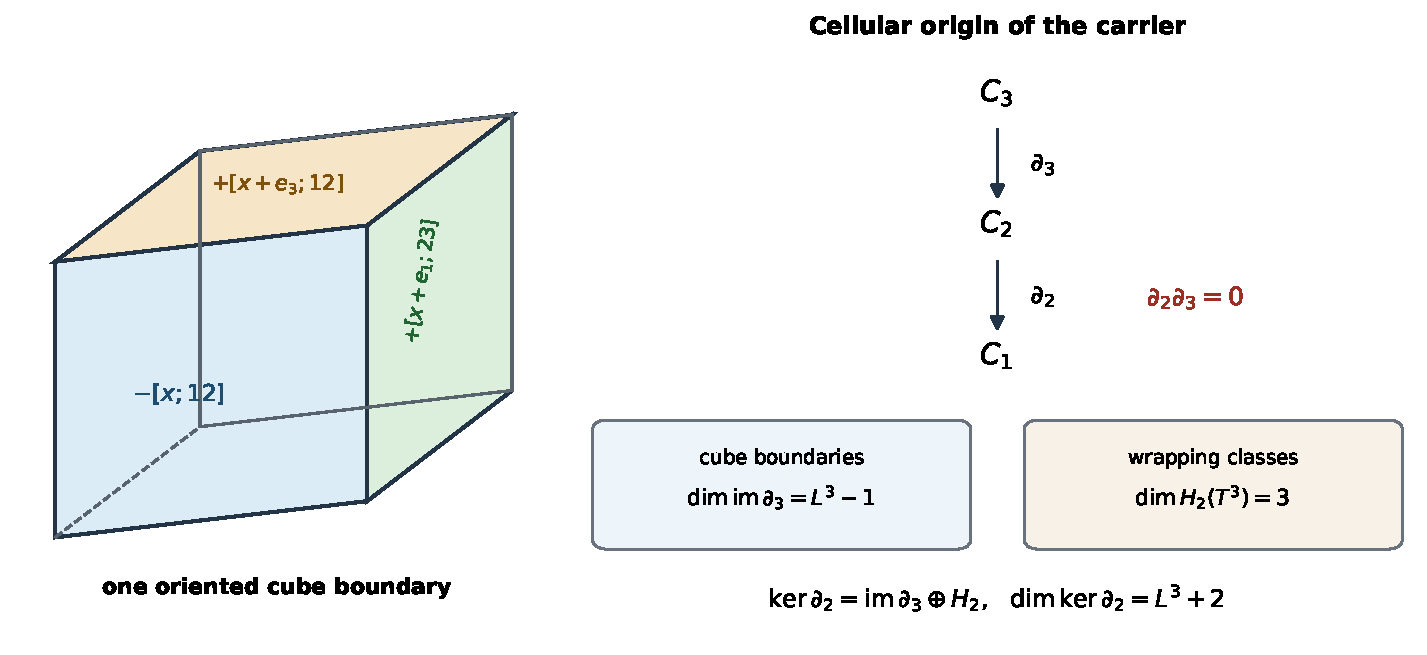
\includegraphics[width=0.97\textwidth]{figure_cellular_carrier.pdf}
\caption{The carrier is a cellular cycle space. The left panel shows three
visible terms in the outward-oriented boundary of one cube; the complete
six-face formula is given in Appendix~\ref{app:chain}. Cube boundaries span
$\operatorname{im}\partial_3$, while three noncontractible wrapping classes
complete $\ker\partial_2$ on the three-torus.}
\label{fig:cellular}
\end{figure}

The count is verified over $\mathbb{Z}$ rather than re-derived from the
formula: the complex is built from the boundary formulas of
Appendix~\ref{app:chain}; the exhibited cycles --- every elementary cube
boundary together with three wrapping sheets --- bound the kernel from below,
and rank over $\mathbb{F}_p$ bounds it from above, since rank can only drop
under reduction. The two bounds meet at $L=1,\dots,5$.
\chk{dim Z\_2 = L\^{}3 + 2 by rank, not by re-arranging the formula}
\chk{cube boundaries and three wrapping sheets SPAN Z\_2}

\begin{remark}
$L^3+2$ is the nullity of the down boundary Laplacian, not a Betti number; the
Betti contribution is the final $3$. The restriction $L\ge3$ belongs to the
twelve-neighbour Bloch adjacency, where $x+e$ and $x-e$ coincide at $L=2$. The
chain-level count has no such restriction and holds at $L=1,2$ as well.
\chk{the L\^{}3+2 count is chain-level, not the Bloch convention}
\end{remark}

The following sum rule joins Theorems~\ref{thm:fact} and~\ref{thm:carrier},
which are otherwise two unrelated statements: a $3\times3$ spectrum and an
$(L^3+2)$-dimensional space.

\begin{theorem}[Bloch--chain bridge]\label{thm:bridge}
On the periodic $L^3$ complex,
\[
  \sum_{k}\bigl(3-\operatorname{rank}B(k)\bigr)=L^3+2 ,
\]
the sum running over the $L^3$ allowed momenta, with nullity profile
$3$ at $\Gamma$ exactly once and $1$ at each of the other $L^3-1$ momenta.
\end{theorem}

\begin{proof}
$B(0)=0$ contributes $3$. For $k\neq0$ some $d_j\neq0$, and
Theorem~\ref{thm:fact} gives $\operatorname{rank}B(k)=2$, contributing $1$
each. Summing gives $3+(L^3-1)=L^3+2$.
\end{proof}
\chk{the Bloch and chain routes to the carrier agree}

\begin{remark}
The two decompositions produce the same two numbers from different objects.
The $3$ is the triple degeneracy of $B(0)=0$, not $b_2(T^3)$; the $L^3-1$
counts non-$\Gamma$ momenta, not cubes. Their agreement is a consistency check
on the whole construction, not a restatement.
\end{remark}

\begin{proposition}[Fixed-momentum carrier and the locality tradeoff]
\label{prop:fixed-k-carrier}
Let $b_x=\partial_3[x;1,2,3]$ be the six-face boundary of the elementary cube
at $x$, and use the unitary discrete Fourier transform
\[
 \widehat b_L(k)=L^{-3/2}\sum_{x\in\Lambda_L}e^{-ik\cdot x}b_x .
\]
For every allowed $k\ne0$, $\widehat b_L(k)$ has norm $\sqrt{q(k)}$ and,
up to the Fourier phase convention, is the vector $w(k)$ of
Theorem~\ref{thm:fact}. Hence
\[
 \phi_L(k)=\frac{\widehat b_L(k)}{\sqrt{q(k)}}
\]
is exactly the unique unit carrier vector in that momentum fibre. If
$k_0=2\pi(r_1,r_2,r_3)/L_0\ne0$, then $k_0$ is an allowed momentum on every
nested volume $L=mL_0$, and the order-$u^2$ internal separation from each of
the two incidence branches is
\begin{equation}\label{eq:fixed-k-splitting}
 t_Nu^2q(k_0),
\end{equation}
independent of $m$. More generally it is bounded below by
$t_Nu^2q_*$ on any set of allowed momenta with $q(k)\ge q_*>0$.

This exact sharp-momentum state is not local: it is the Fourier sum of all
cube boundaries. Conversely, for the normalized radius-one seed
$b_x/\sqrt6$,
\begin{equation}\label{eq:local-fixed-k-weight}
 \left|\langle\phi_L(k),b_x/\sqrt6\rangle\right|^2
 =\frac{q(k)}{6L^3},
\end{equation}
and $\widehat b_L(0)=0$.
\end{proposition}

\begin{proof}
Fourier transforming the six terms of the cubical boundary gives, in the
$(12,13,23)$ face basis, $(d_3,-d_2,d_1)^{\mathsf T}$, with conjugates if the
opposite Fourier sign is chosen. Its squared norm is $q(k)$ and
$\partial_2\partial_3=0$ puts it in $\ker B(k)\dg$; uniqueness for $k\ne0$
follows from Theorem~\ref{thm:fact}. The nested-volume statement is the
integer identity $k_0=2\pi(mr)/(mL_0)$, and
\eqref{eq:fixed-k-splitting} follows from
Corollary~\ref{cor:assembly}. Inverting the unitary Fourier transform gives
$b_x=L^{-3/2}\sum_k e^{ik\cdot x}\sqrt{q(k)}\,\phi_L(k)$, which proves
\eqref{eq:local-fixed-k-weight}; the $k=0$ coefficient vanishes.
\end{proof}

\begin{remark}[What the $L^{-2}$ collapse does and does not say]
The minimum of $q(k)$ over all nonzero finite-volume momenta is
$4\sin^2(\pi/L)$, so a contour isolating the single flat sheet from the other
two sheets uniformly over the entire Brillouin zone cannot follow from the
second-order symbol. This is an \emph{internal} sheet separation. It does not
erase the volume-uniform \emph{external} electric-shell gap
\eqref{eq:external-shell-gap}, and it does not affect the fixed-$k$ coefficient
\eqref{eq:fixed-k-splitting}. Neither fact by itself controls the interacting
Riesz projection or supplies transfer-matrix overlap; those remain the
substantive part of G18.
\end{remark}

\subsection{The wrapping sheets are cycles, not harmonic}

Theorem~\ref{thm:carrier} exhibits its three $H_2$ generators explicitly as
wrapping sheets $s_{(ij)}=\sum_{x:\,x_m=0}[x;i,j]$. These satisfy
$\partial_2 s=0$ exactly, so they are cycles and they span the quotient
$\ker\partial_2/\operatorname{im}\partial_3$. They are \emph{not} harmonic:
$\partial_3\dg s\neq0$, and
\begin{equation}
  \frac{\langle s,\;\partial_3\partial_3\dg\,s\rangle}{\|s\|^2}=2
  \qquad\text{exactly, for every }L\ge2 .
\end{equation}
\chk{FINDING: the wrapping sheets are cycles but NOT harmonic}

The distinction matters because $H_2$ is used in two senses: the quotient in
Theorem~\ref{thm:carrier}, which the sheets span, and the harmonic subspace
$\ker\partial_2\cap\ker\partial_3\dg$, which they do not lie in. Nothing
downstream breaks --- Proposition~\ref{prop:rigid} rests on $B\dg w=0$, which
covers all of $\ker\partial_2$ --- but a real-space statement phrased for the
harmonic subspace does not cover the generators this construction exhibits.

\section{Exact adjacent shared-link dynamics and global assembly}
\label{sec:second}

Two plaquettes sharing a link leave six nonshared fundamental links after the
external contractions. On the shared link the fusion channels depend on the
relative induced orientation,
\begin{equation}\label{eq:fusion}
  F\otimes\bar F=\mathbf{1}\oplus\mathrm{Adj},
  \qquad
  F\otimes F=\Lambda^2F\oplus\mathrm{Sym}^2F ,
\end{equation}
with dimensions and quadratic Casimirs
\begin{equation}\label{eq:table}
\begin{aligned}
  d_{\mathbf 1}&=1, & C_{\mathbf 1}&=0,\\
  d_{\mathrm{Adj}}&=N^2-1, & C_{\mathrm{Adj}}&=N,\\
  d_{\Lambda^2F}&=\tfrac{N(N-1)}2, & C_{\Lambda^2F}&=\tfrac{(N+1)(N-2)}N,\\
  d_{\mathrm{Sym}^2F}&=\tfrac{N(N+1)}2, & C_{\mathrm{Sym}^2F}&=\tfrac{(N-1)(N+2)}N.
\end{aligned}
\end{equation}

The six nonshared half-links contribute $3\CF$ and the fused link $C_\rho/2$,
against an external one-plaquette energy $2\CF$, so the resolvent denominator
is $\CF+C_\rho/2$ exactly.
\chk{each channel gap is C\_F + C\_R/2, and the weights sum to one}

\subsection{The channel weights are a theorem}

Earlier editions assigned the channel projector squared norm $d_\rho/N^2$ by
an isotropy hypothesis, and every statement in this section rests on that
assignment. It is not a hypothesis.

\begin{theorem}[Shared-link channel weights]\label{thm:weingarten}
In the normalised two-plaquette state, the weight of the shared-link channel
$\rho$ is exactly $d_\rho/N^2$, for both orientation families and every
$N\ge3$.
\end{theorem}

\begin{proof}
Two steps. First the six nonshared links collapse. Each plaquette contributes
a product of three independent Haar links, and a product of independent Haar
matrices is Haar, so the amplitude is
$\operatorname{Tr}(AU)\operatorname{Tr}(BU^{\pm1})$ with $A,B$ independent
Haar and $U$ the shared link. Integrating $A$ and $B$ contributes
$\delta/N$ each and leaves a pure degree-$(2,2)$ moment of $U$.

Second, two such moments settle both families. In the Weingarten calculus,
whose asymptotic origin is~\cite{Weingarten1978} and whose finite-$N$ closed
forms are~\cite{CollinsSniady2006}, the order-two values are
$\mathrm{Wg}(e)=1/(N^2-1)$ and
$\mathrm{Wg}((12))=-1/(N(N^2-1))$ --- the inverse of the $S_2$ Gram matrix
$\bigl(\begin{smallmatrix}N^2&N\\N&N^2\end{smallmatrix}\bigr)$ --- the index
sums give
\begin{equation}\label{eq:moments}
  \begin{aligned}
    M_{\mathrm{direct}}&=\sum_{ijkl}\bigl\langle|U_{ij}|^2|U_{kl}|^2\bigr\rangle=N^2,\\
    M_{\mathrm{cross}}&=\sum_{ijkl}\bigl\langle U_{ij}U_{kl}\bar U_{il}\bar U_{kj}\bigr\rangle=N .
  \end{aligned}
\end{equation}
The standard formula is often written for $U(N)$. The present degree-$(2,2)$
integrands are invariant under $U\mapsto zU$, so disintegrating Haar measure
over the central $U(1)$ shows that their normalised $U(N)$ and $SU(N)$
integrals coincide. No determinant-sector term occurs at this degree for
$N\ge3$.
For the like family, $\operatorname{Tr}(AU)\operatorname{Tr}(BU)$ decomposes
into $\mathrm{Sym}^2\oplus\Lambda^2$ by symmetrising the two index pairs
jointly, and the two squared norms are
$(M_{\mathrm{direct}}\pm M_{\mathrm{cross}})/2$. Normalising,
\[
  n_{\mathrm{Sym}^2}=\frac{N+1}{2N}=\frac{d_{\mathrm{Sym}^2F}}{N^2},
  \qquad
  n_{\Lambda^2}=\frac{N-1}{2N}=\frac{d_{\Lambda^2F}}{N^2}.
\]
For the mixed family the singlet component of $U_{ij}\bar U_{lk}$ is
$\delta_{il}\delta_{jk}/N$, of squared norm $1$ against
$M_{\mathrm{direct}}=N^2$, so $n_{\mathbf 1}=1/N^2=d_{\mathbf 1}/N^2$ and
$n_{\mathrm{Adj}}=1-1/N^2=d_{\mathrm{Adj}}/N^2$.
\end{proof}
\chk{the shared-link weights are Weingarten, not an isotropy assumption}

\begin{remark}
The derivation imports nothing: the Weingarten pair is the inverse of the
$S_2$ Gram matrix and the index sums in \eqref{eq:moments} are explicit, so
the reader can check it without leaving this page. That the pair is not two
fitted constants is separately checked --- the identity-permutation value times
$N^2-1$ is $1$ identically in $N$, so the $SU(3)$ numbers are a specialisation
of a rank-generic formula. Together these make the \emph{local shared-link
coefficient} self-contained. By themselves they do not enumerate every
second-order process; that separate step is supplied by
Lemma~\ref{lem:process-complete}. Appendix~%
\ref{app:wg} records the index sums.
\chk{the Weingarten route is independent of the corpus}
\end{remark}

\begin{remark}[External corroboration]
The same numerator appears in the quantum-simulation literature from an
unrelated direction. Ciavarella, Burbano and Bauer~\cite{CBB2025} publish a
finite-rank plaquette matrix element
$|M_\rho|^2=\dim\rho/(\dim A\,\dim R)$; for two fundamental factors
$\dim A=\dim R=N$ and this is $d_\rho/N^2$ identically in $N$. That is
provenance for a chain already checked here, not a second derivation. The
exhaustion of the shared-link routes is proved independently in
Lemma~\ref{lem:process-complete}.
\chk{the published dimension-ratio matrix element is this registry's weight formula}
\end{remark}

\begin{remark}[A falsified zero backend]
The organized authority corpus contains an independent exact diagnostic at
$N=3$:
\[
 \mathrm{Wg}(e)=\frac18,\qquad
 \mathrm{Wg}((12))=-\frac1{24},\qquad
 \int_{SU(3)}|U_{11}|^4\,dU=\frac16\ne0.
\]
It therefore falsifies the archived stranded-flux rule that discards this
balanced Haar sector. This is useful negative evidence for retaining the
contractions above; it is not a second derivation of $t_N$.
\end{remark}

\subsection{The off-diagonal process list is complete}

Write $X_q=\chi_q+\bar\chi_q$, so $V=\sum_qX_q$, and let
$Q_0=1-|0\rangle\langle0|$.

\begin{lemma}[Small-support cellular two-cycles]
\label{lem:small-support-two-cycle}
Fix one orientation for every elementary face of $\Lambda_L$, with $L\ge3$.
If
\[
 z=\sum_f a_ff\in C_2(\Lambda_L;\mathbb Z_N),
 \qquad N\ge2,
\]
satisfies $\partial_2z=0$ and
$|\operatorname{supp}z|\le4$, then $z=0$.
\end{lemma}

\begin{proof}
Suppose $z\ne0$ and choose $f\in\operatorname{supp}z$.  For every one of
the four distinct links $e\subset\partial f$,
\[
 0=(\partial_2z)_e
 =s(f,e)a_f+
 \sum_{\substack{g\ne f\\e\subset\partial g}}s(g,e)a_g .
\]
Since $s(f,e)a_f\ne0$ in $\mathbb Z_N$, at least one other supported face
$g_e$ contains $e$.  For $L\ge3$, two distinct elementary faces of the
periodic cubic complex share at most one link.  The four faces $g_e$ are
therefore distinct, giving $|\operatorname{supp}z|\ge1+4=5$, a
contradiction.
\end{proof}

\begin{remark}
The hypothesis $L\ge3$ is sharp for this lemma: at $L=2$, a coordinate
wrapping sheet contains four faces and is a nonzero cellular two-cycle.
\end{remark}

\begin{lemma}[Reduced same-face route]
\label{lem:reduced-same-face}
For every $N\ge3$ and distinct plaquettes $p,p'$,
\begin{equation}\label{eq:same-face-offdiag}
 \langle p',-|X_{p'}Q_-(E_{F,N}-H_E)^{-1}
 Q_-X_p|p,-\rangle=0 .
\end{equation}
For $SU(3)$ the same matrix element, including the diagonal, is
\begin{equation}\label{eq:su3-same-face-resolvent}
 \langle p',-|X_{p'}Q_-(E_{F,3}-H_E)^{-1}
 Q_-X_p|p,-\rangle=-\frac14\,\delta_{p'p} .
\end{equation}
\end{lemma}

\begin{proof}
Write $\chi_{R,p}$ for the Wilson character in irrep $R$ around $p$ and put
$Y_p=X_p|p,-\rangle$.  The mixed-orientation terms cancel before any
projection:
\[
 \frac{\chi_p\bar\chi_p-\bar\chi_p\chi_p}{\sqrt2}|0\rangle=0 .
\]
Thus the vacuum and adjoint pieces of
$F\otimes\bar F=\mathbf1\oplus\mathrm{Adj}$ are absent, while
\[
 Y_p=\frac{\chi_p^2-\bar\chi_p^2}{\sqrt2}|0\rangle .
\]
For $N\ge4$ this is
\[
 \frac{\chi_{\mathrm{Sym}^2F,p}+\chi_{\Lambda^2F,p}
 -\chi_{\overline{\mathrm{Sym}^2F},p}
 -\chi_{\overline{\Lambda^2F},p}}{\sqrt2}|0\rangle,
\]
with coincident conjugate terms cancelling when an irrep is self-conjugate.
None of the surviving terms belongs to the retained fundamental shell.

For $SU(3)$ the determinant epsilon tensor gives
$\Lambda^2F\simeq\bar F$ and
\[
 \chi_F^2=\chi_{\mathbf6}+\chi_{\bar F},
 \qquad
 \chi_{\bar F}^2=\chi_{\bar{\mathbf6}}+\chi_F .
\]
With
\[
 |p,\mathbf6,-\rangle
 :=\frac{\chi_{\mathbf6,p}-\chi_{\bar{\mathbf6},p}}{\sqrt2}|0\rangle,
\]
one obtains
\begin{equation}\label{eq:su3-same-face}
 X_p|p,-\rangle=|p,\mathbf6,-\rangle-|p,-\rangle,
\end{equation}
and hence
\begin{equation}\label{eq:su3-same-face-Q}
 P_-X_p|p,-\rangle=-|p,-\rangle,
 \qquad
 Q_-X_p|p,-\rangle=|p,\mathbf6,-\rangle .
\end{equation}
The determinant-related fundamental component therefore does not cancel; it
is removed by the reduced-space projector $Q_-$.

Every surviving summand of $Q_-Y_p$ is a one-plaquette spin network supported
on $\partial p$ and carries a nontrivial irrep on each boundary link.  If
$p\ne p'$, some link belongs to exactly one of $\partial p,\partial p'$, so
Peter--Weyl orthogonality separates the two vectors.  The electric Hamiltonian
and its reduced resolvent preserve these spin-network sectors, proving
\eqref{eq:same-face-offdiag}.

At $N=3$,
\[
 H_E|p,\mathbf6,-\rangle
 =2C_2(\mathbf6)|p,\mathbf6,-\rangle
 =\frac{20}{3}|p,\mathbf6,-\rangle,
 \qquad E_{F,3}=\frac83 .
\]
The reduced denominator is $(8/3-20/3)^{-1}=-1/4$, proving
\eqref{eq:su3-same-face-resolvent}.
\end{proof}

\begin{lemma}[Second-order process completeness]\label{lem:process-complete}
For $N\ge3$, $L\ge3$, and distinct plaquettes $p,p'$, define
\begin{align}
 K_{2,-}&=P_-VQ_-(E_{F,N}-H_E)^{-1}Q_-VP_-,
   \label{eq:K2raw}\\
 H^{\mathrm{exc}}_{2,-}
 &=K_{2,-}-E^{(2)}_{\mathrm{vac}}P_-,
 \qquad
 E^{(2)}_{\mathrm{vac}}
 =\langle0|VQ_0(0-H_E)^{-1}Q_0V|0\rangle .
 \label{eq:K2exc}
\end{align}
If $p$ and $p'$ share no link, then
$\langle p',-|K_{2,-}|p,-\rangle=0$. If they share the unique link $e$,
every nonzero intermediate lies in exactly one of
\[
 F\otimes\bar F=\mathbf1\oplus\mathrm{Adj},\qquad
 F\otimes F=\Lambda^2F\oplus\mathrm{Sym}^2F
\]
or the conjugate of the second decomposition. Thus these four shared-link
channels exhaust every off-diagonal second-order process. The conclusion is
preserved by the stated link-Casimir budget cutoff, and more generally by
cutoffs that are functions only of the link Casimirs and therefore act
identically on all four orientation assignments. A general projection inside
the degenerate $2E_{F,N}$ eigenspace need not preserve the non-adjacent
cancellation.
\end{lemma}

\begin{proof}
Expand the external states and both insertions in oriented characters. A term
$\chi_p^\epsilon\chi_q^\eta$, with
$\epsilon,\eta\in\{\pm1\}$ and $\chi^{-1}=\bar\chi$, has linkwise
centre charge $\partial(\epsilon p+\eta q)$ in
$C_1(\Lambda_L;\mathbb Z_N)$. Since $H_E$ commutes with the independent
link-centre actions, a common electric intermediate between the $p$ and $p'$
sides requires
\begin{equation}\label{eq:centre-match}
 \partial(\epsilon p+\eta q)
 =\partial(\epsilon'p'+\eta'r)\pmod N
\end{equation}
for action plaquettes $q,r$ and signs
$\epsilon,\eta,\epsilon',\eta'$.

Apply Lemma~\ref{lem:small-support-two-cycle} to
\[
 z=\epsilon p+\eta q-\epsilon'p'-\eta'r .
\]
Equation~\eqref{eq:centre-match} gives $\partial_2z=0$, and the support has at
most four faces, so $z=0$ in $C_2(\Lambda_L;\mathbb Z_N)$. For $N\ge5$,
every face coefficient has absolute value at most four, so modular vanishing
is ordinary integral cancellation. For $N=3$, a non-paired coefficient could
vanish only by being $\pm3$; this would use three occurrences on one face and,
because $p\ne p'$, leave a distinct face with coefficient $\pm1$. For $N=4$,
a non-paired coefficient could vanish only by being $\pm4$, which would put
all four occurrences on one face and again contradict $p\ne p'$. Therefore
the four occurrences pair with opposite signs, and the only possibilities are
\begin{align}
 q&=p,\quad \eta=-\epsilon,
 &r&=p',\quad \eta'=-\epsilon',
 \label{eq:zero-route}\\
 \intertext{or}
 q&=p',\quad r=p,
 &\eta&=\epsilon',\quad \eta'=\epsilon .
 \label{eq:exchange-route}
\end{align}

The alternative~\eqref{eq:zero-route} is the same-face route of
Lemma~\ref{lem:reduced-same-face}. Its mixed-orientation vacuum and adjoint
pieces cancel algebraically. At $N=3$ the full same-face vector also contains
the determinant-induced retained-shell term $-|p,-\rangle$, but
\eqref{eq:su3-same-face-Q} shows that $Q_-$ removes it. The surviving sextet
route is diagonal by~\eqref{eq:su3-same-face-resolvent}. Therefore only
\eqref{eq:exchange-route} can contribute off diagonal. If $p,p'$ are
link-disjoint, sharing
a vertex being immaterial, linkwise factorisation gives
\[
 X_{p'}|p,-\rangle=\sqrt2\,|p,-\rangle|p',+\rangle,
 \qquad
 X_p|p',-\rangle=\sqrt2\,|p,+\rangle|p',-\rangle .
\]
Both vectors have electric energy $2E_{F,N}$, so the reduced resolvent is
scalar on their span, while their inner product is zero by charge
orthogonality.

If $p,p'$ share $e$, the six nonshared links each carry one fundamental or
antifundamental factor and the shared link carries exactly two. The two
complete tensor-product decompositions above therefore give all common
intermediates. Their energies and gaps are
\[
 E_\rho=3\CF+\frac12C_\rho,\qquad
 E_\rho-E_{F,N}=\CF+\frac12C_\rho>0 .
\]
Spectral resolution yields only their four projectors. Vacuum subtraction is
diagonal and leaves this cross matrix element unchanged. The two-face term is
connected, so the linked M\"obius projection leaves it unchanged as well.
\end{proof}
\chk{second-order off-diagonal processes are exactly the adjacent shared-link channels}

With Theorem~\ref{thm:weingarten} the resolvent weight is
\begin{equation}\label{eq:w}
  w_\rho=-\frac{d_\rho/N^2}{\CF+C_\rho/2},
\end{equation}
and summing within the two orientation families,
\begin{align}
  A_N&=w_{\mathbf 1}+w_{\mathrm{Adj}}=-\frac{2N^3}{(N^2-1)(2N^2-1)},\label{eq:AN}\\
  B_N&=w_{\Lambda^2}+w_{\mathrm{Sym}^2}=-\frac{4N(N^2-2)}{(N^2-1)(4N^2-9)}.\label{eq:BN}
\end{align}
\chk{the four channel weights follow from dimension and Casimir}
\chk{A\_N and B\_N are the channel sums, not transcriptions}

\subsection{The shared-link law}

\begin{theorem}[All-rank adjacent shared-link law]\label{thm:allrank}
Let $p\ne p'$ be oriented plaquettes sharing the single link $e$. For every
integer $N\ge3$, let $s=s(p,e)$, $s'=s(p',e)$, and let
$\widehat\Pi_\rho$ be the charge-conjugation-closed electric projector onto
the shared-link channel $\rho$ (including the conjugate irrep on the
conjugate like-channel subspace). Define
\[
 \eta_\rho=
 \begin{cases}
 -1,&\rho\in\{\mathbf1,\mathrm{Adj}\},\\
 +1,&\rho\in\{\Lambda^2F,\mathrm{Sym}^2F\}.
 \end{cases}
\]
Then
\begin{align}
 \widehat\Pi_\rho X_{p'}|p,-\rangle
 &=\eta_\rho ss'\widehat\Pi_\rho X_p|p',-\rangle,
 \qquad
 \bigl\|\widehat\Pi_\rho X_{p'}|p,-\rangle\bigr\|^2
 =\frac{d_\rho}{N^2}.\label{eq:projected-route}
\end{align}
\begin{equation}\label{eq:projector-cross}
 \boxed{\;
 \langle p',-|X_p\widehat\Pi_\rho X_{p'}|p,-\rangle
 =\eta_\rho s(p',e)s(p,e)\frac{d_\rho}{N^2}
 \;} .
\end{equation}
Consequently the linked order-$u^2$ contribution through all four channels is
\[
  \langle p',-|H_2|p,-\rangle
  =t_N\,s(p',e)s(p,e)
  =t_N(BB\dg)_{p'p},
\]
where $s(p,e)=\pm1$ is the cellular boundary incidence and
\[
  t_N=B_N-A_N=\frac{2N(N^2-4)}{(N^2-1)(2N^2-1)(4N^2-9)}>0 .
\]
\end{theorem}

\begin{proof}
Because distinct cubical faces share at most one link,
$(BB\dg)_{p'p}=ss'$. Expand
\[
 |p;\epsilon\rangle_{\mathrm{or}}:=\chi_p^\epsilon|0\rangle,\qquad
 \chi_p^{+1}:=\chi_p,\quad\chi_p^{-1}:=\bar\chi_p,
 \qquad
 |p,-\rangle=2^{-1/2}\sum_{\epsilon=\pm1}
   \epsilon|p;\epsilon\rangle_{\mathrm{or}} .
\]
Put $\sigma=ss'$. On the shared link the two oriented factors are
$\epsilon s$ and $\epsilon's'$. The complete orientation bookkeeping is
\begin{equation}\label{eq:orientation-channel-table}
\begin{array}{c|c|c|c|c}
 \rho
 & \text{shared-link family}
 & \epsilon\epsilon'
 & \eta_\rho
 & \eta_\rho ss'\,d_\rho/N^2
 \\ \hline
 \mathbf1
 & F\otimes\bar F\ \text{or}\ \bar F\otimes F
 & -\sigma & -1
 & -ss'/N^2
 \\
 \mathrm{Adj}
 & F\otimes\bar F\ \text{or}\ \bar F\otimes F
 & -\sigma & -1
 & -ss'(N^2-1)/N^2
 \\
 \Lambda^2F\ \text{and its conjugate}
 & F\otimes F\ \text{or}\ \bar F\otimes\bar F
 & \sigma & +1
 & ss'(N-1)/(2N)
 \\
 \mathrm{Sym}^2F\ \text{and its conjugate}
 & F\otimes F\ \text{or}\ \bar F\otimes\bar F
 & \sigma & +1
 & ss'(N+1)/(2N)
\end{array}
\end{equation}
For a fixed monomial $\chi_p^\epsilon\chi_{p'}^{\epsilon'}$, the forward
route carries charge-odd coefficient $\epsilon/\sqrt2$, whereas the reversed
route carries $\epsilon'/\sqrt2$. Their ratio is
$\epsilon/\epsilon'=\epsilon\epsilon'$. Opposite induced orientations give
$\epsilon\epsilon'=-ss'$ and the mixed family; equal induced orientations
give $\epsilon\epsilon'=ss'$ and the like family. Hence
\[
 \widehat\Pi_\rho X_{p'}|p,-\rangle
 =\eta_\rho ss'\widehat\Pi_\rho X_p|p',-\rangle .
\]
The two charge-conjugate assignments are orthogonal for $N\ge3$, so their two
external factors combine to the single channel norm $d_\rho/N^2$.
This proves \eqref{eq:projected-route} and \eqref{eq:projector-cross}.

On this channel,
\[
 (E_{F,N}-H_E)^{-1}\widehat\Pi_\rho
 =-\frac{\widehat\Pi_\rho}{\CF+C_\rho/2}.
\]
Its contribution is therefore $\eta_\rho ss'w_\rho$. Summing gives
\[
 ss'\bigl(
 w_{\Lambda^2F}+w_{\mathrm{Sym}^2F}
 -w_{\mathbf1}-w_{\mathrm{Adj}}\bigr)
 =ss'(B_N-A_N).
\]
Substitution of \eqref{eq:AN}--\eqref{eq:BN} gives the displayed rational
function. Every denominator factor and $N^2-4$ is positive for $N\ge3$.
\end{proof}
\chk{t\_N = B\_N - A\_N}\chk{t\_N > 0 for N >= 3}

\begin{corollary}[Global torus assembly]\label{cor:assembly}
On the trivial-flux charge-odd electric shell of
Theorem~\ref{thm:retained-shell}, translation and cubic symmetry make the
remaining diagonal contribution a scalar.  More precisely, there is a scalar
$d_{2,N,L}$, computed in closed form and shown $L$-independent in
Theorem~\ref{thm:scalar-ledger} below, such that
\[
 [u]H^{(N)}_{\mathrm{eff},-}(k,u)=\delta_{N,3}I,
 \qquad
 [u^2]H^{(N)}_{\mathrm{eff},-}(k,u)
 =d_{2,N,L}I+t_NB(k)B(k)\dg .
\]
Equivalently, with
$E_{\mathrm{flat},N,L}^{[2]}(u)=E_{F,N}+\delta_{N,3}u+d_{2,N,L}u^2$,
\[
  T_{\le2}H^{(N)}_{\mathrm{eff},-}(k,u)
  =E_{\mathrm{flat},N,L}^{[2]}(u)I+t_Nu^2B(k)B(k)\dg .
\]
Consequently the three band Taylor polynomials through second order are
$E_{\mathrm{flat},N,L}^{[2]}(u)$ and
$E_{\mathrm{flat},N,L}^{[2]}(u)+t_Nu^2q(k)$ twice.  This is a coefficient
identity, not a claim of a remainder uniform in $L$.
\end{corollary}

\begin{proof}
The centre-charge argument of Lemma~\ref{lem:process-complete}, now with only
three plaquette occurrences, gives
$\langle p',-|P_-VP_-|p,-\rangle=0$ for $p\ne p'$. A possible $SU(3)$
determinant balance would require all three occurrences to be the same face
and is therefore excluded off diagonal. On the diagonal it occurs only at
$N=3$, where \eqref{eq:su3-same-face-Q} gives
\[
 P_-VP_-=-\delta_{N,3}P_-,
 \qquad
 [u]H^{(N)}_{\mathrm{eff},-}=-P_-VP_-=\delta_{N,3}I .
\]

At second order Lemma~\ref{lem:process-complete} and
Theorem~\ref{thm:allrank} assemble every off-diagonal entry. Translations act
transitively on faces of a fixed orientation and the cubic group permutes the
orientations, so the invariant second-order diagonal is also a multiple of the
identity. Thus the adjacency part is
$t_N(BB\dg-4I)$; absorb $-4t_N$ into the scalar and apply
Theorem~\ref{thm:fact}.
\end{proof}

Two consequences,
\begin{equation}\label{eq:tsmall}
  t_3=\frac{5}{612},\qquad
  t_N=\frac1{4N^3}-\frac1{16N^5}-\frac{77}{64N^7}-\frac{1021}{256N^9}+\cdots
\end{equation}
\chk{t\_2 = 0 and t\_3 = 5/612}\chk{large-N expansion of t\_N through 1/N\^{}9}

The expansion is governed by a closed form. Writing the planar-normalised
coefficient as $4N^3t_N$,
\begin{equation}\label{eq:planar}
  1-4N^3t_N=\frac{2N^4+31N^2-9}{(N^2-1)(2N^2-1)(4N^2-9)}.
\end{equation}
Identity \eqref{eq:planar} holds between rational functions
\leanref{hopping\_deficit\_numerator}; the right side is positive and the
left strictly decreasing for every real
$N\ge2$: substituting $N=M+2$ makes every numerator coefficient of both the
remainder and the derivative nonnegative, so $4N^3t_N$ increases monotonically
to $1$. At fixed canonical coordinate $u$ the width of
Corollary~\ref{cor:assembly} is $12t_Nu^2$, so the entire dispersive content
of the projected sector switches off at exactly the rate $N^{-3}$, with
computable subleading coefficient $-1/(4N^2)$. This is consistent with the
general suppression of glueball mixing at large $N$, but no 't~Hooft-coupling
identification is made here. The channel algebra behind $t_N$ --- the four
closed-form weights, the two family sums, and the weights summing to one per
family --- is proof-checked as well \leanref{mixed\_family\_sum},
\leanref{like\_family\_sum}, \leanref{family\_weights\_sum\_to\_one}.
\chk{deficit identity 1/4 - N\^{}3 t\_N}
\chk{N\^{}3 t\_N increases monotonically to 1/4}

\subsection{The vacuum-mediated route}

Lemma~\ref{lem:process-complete} is specific to the charge-odd shell. The
corresponding assertion is false in general: the charge-even sector admits a
vacuum-mediated route. Its cancellation in the odd sector is the
charge-conjugation selection rule below.

\begin{proposition}[Vacuum-mediated route]\label{prop:vacuum}
The reduced-resolvent route
\[
 \frac{\langle p'|V|0\rangle\langle 0|V|p\rangle}{E_{F,N}-E_0}
 =\frac{\langle p'|V|0\rangle\langle 0|V|p\rangle}{E_{F,N}}
\]
is available for any
pair of plaquettes, sharing a link or not. It vanishes identically in the
charge-odd sector, because $V$ is charge-even and $|0\rangle$ is charge-even,
so $\langle0|V|p,-\rangle=0$. Consequently the charge-odd hopping
$t_N=B_N-A_N$ carries no such term, while the charge-even shared-link element
acquires $1/\CF$: the normalised charge-even matrix-element product is $2$
and $E_{F,N}=2\CF$.
\[
  \ell_N=A_N+B_N+\frac1{\CF}
  =-\frac{2N(3N^2-5)}{(N^2-1)(2N^2-1)(4N^2-9)} .
\]
\end{proposition}
\chk{ell\_N = A\_N + B\_N + 1/C\_F, the vacuum-mediated route at every rank}

\begin{remark}
At $N=3$, $A_3+B_3=-481/612$ and $1/\CF=3/4$, giving $\ell_3=-11/306$. The
first of these is exactly the value once published for the charge-even hopping
and later superseded; the correction is precisely the omitted route. Stating
the selection rule turns a one-rank erratum into an all-rank formula.

In the charge-odd shell, Lemma~\ref{lem:process-complete} and this proposition
dispose of non-adjacent pairs: the exchange vectors are orthogonal and the
vacuum route vanishes. In the charge-even sector the non-adjacent vacuum route
does not vanish, and revision 5 read it as a rank-one all-pairs operator whose
cancellation ``has not been derived'' and ``remains a separate requirement''.
Those two sentences were stale against this paper's own corpus: the flat-band
manuscript's lemma on the vacuum-mediated route, and the June 2026 patch to
its Section~6, state at $N=3$ that the route $+\tfrac34$ ``exactly cancels the
free two-flux channel sum $2/(8/3-16/3)=-\tfrac34$, recovering the vanishing
of distant hops''. They are withdrawn. The theorem below is that sentence
lifted to every rank and to an operator identity, with the adjacent element's
orientation independence proved monomial by monomial.
\chk{FINDING: revision 5 called the charge-even vacuum-route cancellation underived; the pinned corpus proves it for distant pairs at N = 3}
\end{remark}

\begin{theorem}[Charge-even second-order symbol]\label{thm:even-symbol}
For $N\ge3$, $L\ge3$ and distinct plaquettes $p,p'$, with $K_{2,+}$ and
$H^{\mathrm{exc}}_{2,+}$ defined as in \eqref{eq:K2raw}--\eqref{eq:K2exc}
with $P_+$ in place of $P_-$,
\[
 \langle p',+|H^{\mathrm{exc}}_{2,+}|p,+\rangle=
 \begin{cases}\ell_N,& p,p'\text{ share a link},\\ 0,& \text{otherwise},\end{cases}
\]
independently of the boundary orientations. Consequently
\[
 [u^2]H^{(N)}_{\mathrm{eff},+}(k,u)
 =d^+_{2,N}I+\ell_N\bigl(\mathcal N(k)\mathcal N(k)\dg-4I\bigr),
\]
with $\mathcal N(k)$ the unsigned incidence of Section~\ref{sec:second} and
$d^+_{2,N}$ the scalar of Theorem~\ref{thm:scalar-ledger}.
\end{theorem}

\begin{proof}
The centre-charge argument of Lemma~\ref{lem:process-complete} is blind to
charge parity, so the only routes are the same-face route
\eqref{eq:zero-route} and the exchange route \eqref{eq:exchange-route}.

\emph{Link-disjoint pairs.} Expanding
$X_p|p,+\rangle=(\chi_p+\bar\chi_p)^2|0\rangle/\sqrt2$ by
$\chi_F^2=\chi_{\mathrm{Sym}^2F}+\chi_{\Lambda^2F}$ and
$\chi_F\bar\chi_F=1+\chi_{\mathrm{Adj}}$, its vacuum component is
$\sqrt2\,|0\rangle$ and every other component carries flux on $\partial p$,
which $X_{p'}$ cannot remove; so the same-face route contributes exactly the
vacuum route
$\langle p',+|X_{p'}|0\rangle\langle0|X_p|p,+\rangle/(E_{F,N}-0)=2/E_{F,N}$.
(At $N=3$ the retained component $|p,+\rangle$ is removed by $Q_+$, and could
not reach $\langle p',+|$ in any case.) The exchange route goes through
$X_{p'}|p,+\rangle=\sqrt2\,|p,+\rangle|p',+\rangle=X_p|p',+\rangle$, one
vector at energy $2E_{F,N}$, and contributes
$2/(E_{F,N}-2E_{F,N})=-2/E_{F,N}$. The two cancel
\leanref{disjoint\_pair\_cancels}. In the charge-odd sector both vanish
separately: $\langle0|V|p,-\rangle=0$ and the two exchange vectors are
orthogonal.

\emph{Adjacent pairs.} The vacuum route contributes $2/E_{F,N}=1/\CF$ as
before. In the exchange route, expand both states in oriented characters as
in the proof of Theorem~\ref{thm:allrank}. Every monomial
$\chi_{p'}^{\epsilon'}\chi_p^{\epsilon}$ now carries coefficient $1/\sqrt2$ on
both sides, and the bra fixes the nonshared-link fluxes, so
$\langle p';\epsilon'|X_p\widehat\Pi_\rho X_{p'}|p;\epsilon\rangle=d_\rho/N^2$
when $\rho$ lies in the family selected by $(\epsilon s,\epsilon's')$ and
vanishes otherwise. Each family is selected by exactly two of the four
monomials, so every channel contributes $w_\rho$ with sign $+1$, whatever
$s,s'$: the total is $A_N+B_N+1/\CF=\ell_N$. Repeating the count with the
charge-odd coefficients $\epsilon\epsilon'/2$ gives $ss'(B_N-A_N)$, which is
Theorem~\ref{thm:allrank}.

The off-diagonal is therefore $\ell_N$ on every adjacent pair, orientation
independent, which is the unsigned adjacency $\mathcal N\mathcal N\dg-4I$.
Translation and cubic symmetry make the diagonal a scalar, as in
Corollary~\ref{cor:assembly}.
\end{proof}
\chk{the charge-even second-order symbol is ell\_N times the unsigned incidence: the vacuum route cancels the doubly-excited route on every link-disjoint pair}

\begin{remark}[Regime, and an outside corroboration]
This is a finite-volume coefficient identity, exactly as
Corollary~\ref{cor:assembly} is: at $k=0$ the $A_1^{++}$ combination couples
to the vacuum with an extensive matrix element, so no remainder uniform in
$L$ is claimed. What the theorem changes is the standing of
Section~\ref{sec:even}: the unsigned symbol is the charge-even sector at
order $u^2$, and its $\Gamma$-point splitting $12\ell_N$ and bandwidth
$16|\ell_N|$ (for even $L$, and coefficientwise as $L\to\infty$) are
unconditional. At $N=3$ the theorem is corroborated from outside. An
independent engine, built on the corpus's Haar primitives and reading no
register value, returns the charge-even shared-link element $-11/306$ on the
coplanar and on the perpendicular pair alike and $0$ on a link-disjoint pair
(Section~\ref{sec:outside}); and Hamer's $0^{++}$ series matches the
$\Gamma$-point coefficient the theorem predicts (Section~\ref{sec:external}).
\end{remark}

\subsection{The second-order scalar at every rank}\label{sec:scalar}

Corollary~\ref{cor:assembly} proves that the second-order diagonal is a
scalar and, through revision 5, wrote it down only at $N=3$, as the upstream
identification $\mathrm{leak}_2=\ell_3$ with a within-plaquette tower. It is
determined by the same three inputs as the hopping. Write $\sigma^\pm_N$ for
the reduced same-face route
$\langle p,\pm|X_pQ_\pm(E_{F,N}-H_E)^{-1}Q_\pm X_p|p,\pm\rangle$ of
Lemma~\ref{lem:reduced-same-face}.

\begin{theorem}[Second-order scalar ledger]\label{thm:scalar-ledger}
For $N\ge3$ and $L\ge3$ the on-site coefficients are $L$-independent,
\begin{equation}\label{eq:onsite}
 d^\pm_{2,N}=\sigma^\pm_N+\frac1\CF+12\,\ell_N ,
\end{equation}
so that $d_{2,N,L}=d^-_{2,N}-4t_N$ in Corollary~\ref{cor:assembly}, which is
the flat scalar, and in the charge-even sector the $A_1^{++}$ level at
$\Gamma$ is $d^+_{2,N}+12\ell_N$ and the $\lambda=-4$ level $d^+_{2,N}-4\ell_N$.
The same-face routes are, for $N\ge5$,
\begin{align}
 \sigma^-_N&=-\frac{N}{(N-1)(N+3)}-\frac{N}{(N+1)(N-3)}
 =-\frac{2N(N^2-3)}{(N^2-1)(N^2-9)},\label{eq:sigma-odd}\\
 \sigma^+_N&=\frac1\CF-\frac{2N}{N^2+1}+\sigma^-_N,\label{eq:sigma-even}
\end{align}
the two denominators of \eqref{eq:sigma-odd} being the two-flux gaps
$E_{F,N}-2C_2(\mathrm{Sym}^2F)=-(N-1)(N+3)/N$ and
$E_{F,N}-2C_2(\Lambda^2F)=-(N+1)(N-3)/N$ \leanref{two\_flux\_gaps}, and
$-2N/(N^2+1)$ the adjoint gap $E_{F,N}-2N$ with the doubled adjoint norm
\leanref{adjoint\_gap}. At the two exceptional ranks
\[
 \sigma^-_3=-\tfrac14,\quad \sigma^+_3=-\tfrac1{10},\qquad
 \sigma^-_4=-\tfrac4{21},\quad \sigma^+_4=-\tfrac{1028}{595}:
\]
at $N=3$ only the sextet survives $Q_\pm$ and the vacuum and adjoint pieces of
$\sigma^+_3$ are $\tfrac34$ and $-\tfrac35$; at $N=4$ the real six of $su(4)$
cancels in the odd combination and enters doubled in the even one.
Consequently, for $N\ge5$, the charge-odd tower is
\begin{equation}\label{eq:tower}
 \sigma^-_N+\frac1\CF=-\frac{12N}{(N^2-1)(N^2-9)},
\end{equation}
of order $N^{-3}$: the same-face route and the vacuum bubble, each of order
$N^{-1}$, cancel at leading order \leanref{towerOdd\_closed}.
\end{theorem}

\begin{proof}
Lemma~\ref{lem:process-complete} assumes $p\ne p'$; the diagonal case is its
extension. With $p'=p$ the centre-charge chain is
$z=(\epsilon-\epsilon')p+\eta q-\eta'r$, of support at most three, so
Lemma~\ref{lem:small-support-two-cycle} gives $z=0$ in
$C_2(\Lambda_L;\mathbb Z_N)$. If $q$, $r$ and $p$ are distinct the coefficient
$\eta=\pm1$ of $q$ cannot vanish; if exactly one of $q,r$ equals $p$ the other
carries $-\eta'\ne0$; so $q=r$. For $q=r\ne p$ the coefficients
$\epsilon-\epsilon'$ and $\eta-\eta'$ lie in $\{0,\pm2\}$ and $\pm2\ne0$ mod
$N$ for $N\ge3$, so the four monomials of $X_q|p,\pm\rangle$ are pairwise
orthogonal. For $q=r=p$ the single coefficient
$\epsilon+\eta-\epsilon'-\eta'\in\{0,\pm2,\pm4\}$ can vanish mod $4$ at $N=4$
through $(+,+,-,-)$: that is the real six of $su(4)$ shared by
$\chi_p^2|0\rangle$ and $\bar\chi_p^2|0\rangle$, and the same-face route is
decomposed by irreps below, which covers it. Hence
$\langle p|K_2|p\rangle=\sum_q\langle p|X_qQ(E_{F,N}-H_E)^{-1}QX_q|p\rangle$,
with three kinds of $q$. For $q=p$ this is $\sigma^\pm_N$. For the twelve $q$
sharing a link with $p$, $X_q|p,\pm\rangle$ is a sum of four mutually
orthogonal unit monomials, two in each orientation family, each carrying
coefficient squared $\tfrac12$, so the resolvent gives $A_N+B_N$ per
neighbour in either sector. For the $3L^3-13$ link-disjoint $q$,
$X_q|p,\pm\rangle=\sqrt2\,|p,\pm\rangle|q,+\rangle$ at energy $2E_{F,N}$, worth
$-2/E_{F,N}=-1/\CF$ each. The vacuum subtraction is
$E^{(2)}_{\mathrm{vac}}=-3L^3\cdot2/E_{F,N}=-3L^3/\CF$, since
$\|X_q|0\rangle\|^2=2$ for every $q$. Adding,
$\sigma^\pm_N+12(A_N+B_N)+13/\CF$, which is \eqref{eq:onsite}: thirteen
bubbles survive the subtraction, one for $p$ itself and one per neighbour,
and that is why the per-neighbour leakage is $\ell_N$ rather than the bare
channel sum.

For the same-face route,
$X_p|p,\pm\rangle=(\chi_p+\bar\chi_p)(\chi_p\pm\bar\chi_p)|0\rangle/\sqrt2$,
which is $(\chi_p^2-\bar\chi_p^2)/\sqrt2$ in the odd sector and
$(\chi_p^2+2\chi_p\bar\chi_p+\bar\chi_p^2)/\sqrt2$ in the even one. With
$\chi_F^2=\chi_{\mathrm{Sym}^2F}+\chi_{\Lambda^2F}$ and
$\chi_F\bar\chi_F=1+\chi_{\mathrm{Adj}}$, a single-plaquette loop in irrep $R$
costs $2C_2(R)$, and each distinct character has unit norm. For $N\ge5$ the
four like irreps are distinct and none is fundamental, giving
\eqref{eq:sigma-odd} and, with the vacuum at energy $0$ (squared norm $2$)
and the adjoint at $2N$ (squared norm $2$), \eqref{eq:sigma-even}. At $N=4$,
$\Lambda^2F$ is self-conjugate, so $\chi_{\Lambda^2F}-\bar\chi_{\Lambda^2F}$
vanishes and $\chi_{\Lambda^2F}+\bar\chi_{\Lambda^2F}$ has squared norm $4$.
At $N=3$, $\Lambda^2F=\bar F$ and the term is the retained-shell component
$\mp|p,\pm\rangle$ of Lemma~\ref{lem:reduced-same-face}, removed by $Q_\pm$.
Equation~\eqref{eq:tower} is rational arithmetic.
\end{proof}
\chk{the second-order on-site scalar is closed form at every rank: same-face route + 1/C\_F + 12 ell\_N, and L cancels}
\chk{the same-face route is exceptional at N = 3 and N = 4: Lambda\^{}2 F is the conjugate fundamental, then self-conjugate}

\begin{remark}[The ledger at low rank]
At $N=3$ the theorem returns the register: tower $\tfrac12=-\tfrac14+\tfrac34$,
on-site $\tfrac7{102}$, flat $\tfrac{11}{306}$; charge even, tower
$\tfrac{13}{20}$, on-site $\tfrac{223}{1020}$, $A_1^{++}$ at $\Gamma$
$-\tfrac{217}{1020}$, band top $\tfrac{1109}{3060}$
\leanref{su3\_odd\_ledger}, \leanref{su3\_even\_ledger}. Every one of these
was recorded upstream as an identification; each is now a consequence, and
the independent engine of Section~\ref{sec:outside} returns the two same-face
routes $-\tfrac14$ and $-\tfrac1{10}$, the per-neighbour leakage
$-\tfrac{481}{612}$ before and $-\tfrac{11}{306}$ after the neighbour's
$-\tfrac34$ vacuum bubble is subtracted, and $0$ on a link-disjoint pair,
from the primitives --- the last of
these printed in the run's console log rather than its certificate. A second
confirmation at $N=3$ shares nothing with that engine: the two-cube delivery
of Section~\ref{sec:twocube}, built from Clebsch--Gordan amplitudes and folded
at operator level, has a connected diagonal $D_{\mathcal B=6}$ that is the
per-neighbour ledger face by face. The M\"obius weights cancel the same-face
route on every face, and what remains is the cross-cell census: a side face
has one shared-link neighbour and four link-disjoint faces in the other cube,
$-\tfrac{481}{612}+4(-\tfrac34)=-\tfrac{2317}{612}$; an end cap has five
disjoint ones, $-\tfrac{15}4$; the shared face folds to $0$. So the diagonal
Proposition~\ref{prop:orbit} calls the open boundary is the boundary count of
this theorem. (``Linked'' here means vacuum-subtracted on the torus, as in
\eqref{eq:K2exc}; the prism's M\"obius diagonal subtracts sub-complex
operators instead, and the two prescriptions agree on the cross-cell
off-diagonal, which is all Proposition~\ref{prop:split} uses.) At $N=4$ the
odd tower is $\tfrac{12}{35}$, the on-site $\tfrac{10828}{59675}$ and the
flat $\tfrac{9932}{59675}$ \leanref{su4\_ledger}; at $N=5$ the tower is
$-\tfrac5{32}$, the on-site $-\tfrac{4785}{20384}$ and the flat
$-\tfrac{4945}{20384}$ \leanref{flatOdd\_five}. Appendix~\ref{app:ledger-n}
tabulates $N=3$ to $7$. In $1/N$ the flat scalar is $-22/N^3+O(N^{-5})$, the
even $A_1^{++}$ level at $\Gamma$ is $-26/N^3+O(N^{-5})$, and
$\ell_N=-\tfrac34N^{-3}+O(N^{-5})$: every second-order coefficient of the
projected sector, scalar or dispersive, is $O(N^{-3})$ in canonical $u$. One
boundary is worth stating plainly. The $N\ge4$ entries rest on this paper's
algebra and on the verifier's checks of it, and on nothing else: no engine
independent of this derivation has computed a second-order diagonal at any
rank above three. A Haar-exact or Clebsch--Gordan second-order run at $N=4$,
where $\Lambda^2F$ is real and both exceptional mechanisms are exercised at
once, would be the first genuine test of the ledger beyond $SU(3)$.
\chk{at N = 3 the all-rank second-order ledger is the register and an independent engine's table, line by line}
\chk{the two-cube B=6 connected diagonal is the per-neighbour ledger face by face: one shared-link neighbour and four disjoint faces in the other cube}
\chk{the large-N second-order ledger: the towers and flat scalar are O(N\^{}-3), and the leading same-face and bubble terms cancel}
\end{remark}

\subsection{Finite-volume width}

Let $q_{\max}(L)$ be the largest sampled $q$ on the periodic $L^3$ grid. Then
\begin{equation}\label{eq:qmax}
  q_{\max}(L)=
  \begin{cases}
    12, & L\text{ even},\\[2pt]
    12\cos^2\!\bigl(\pi/2L\bigr), & L\text{ odd},
  \end{cases}
\end{equation}
because only at even $L$ does some $k_j$ reach $\pi$ exactly. The width of the
second-order truncated retained charge-odd manifold is exactly
\[
 W^{(-),[2]}_{N,L}(u)=q_{\max}(L)\,t_Nu^2 .
\]
Thus for even $L$, and coefficientwise as $L\to\infty$ at fixed perturbative
order, its $u^2$ coefficient is $12t_N\sim3/N^3$.  No volume-uniform
third-order remainder is asserted.
This concerns the stiffness of the dispersive doublet, not motion of the
lowest branch, which is flat at this order.
\chk{the zone maximum of q is 12 only at even L}

The smallest nonzero incidence eigenvalue is $q_{\min}=4\sin^2(\pi/L)$,
attained by one unit of momentum in a single direction.
\chk{q\_min on the L-torus grid is 4 sin\^{}2(pi/L)}

\begin{figure}[t]
\centering
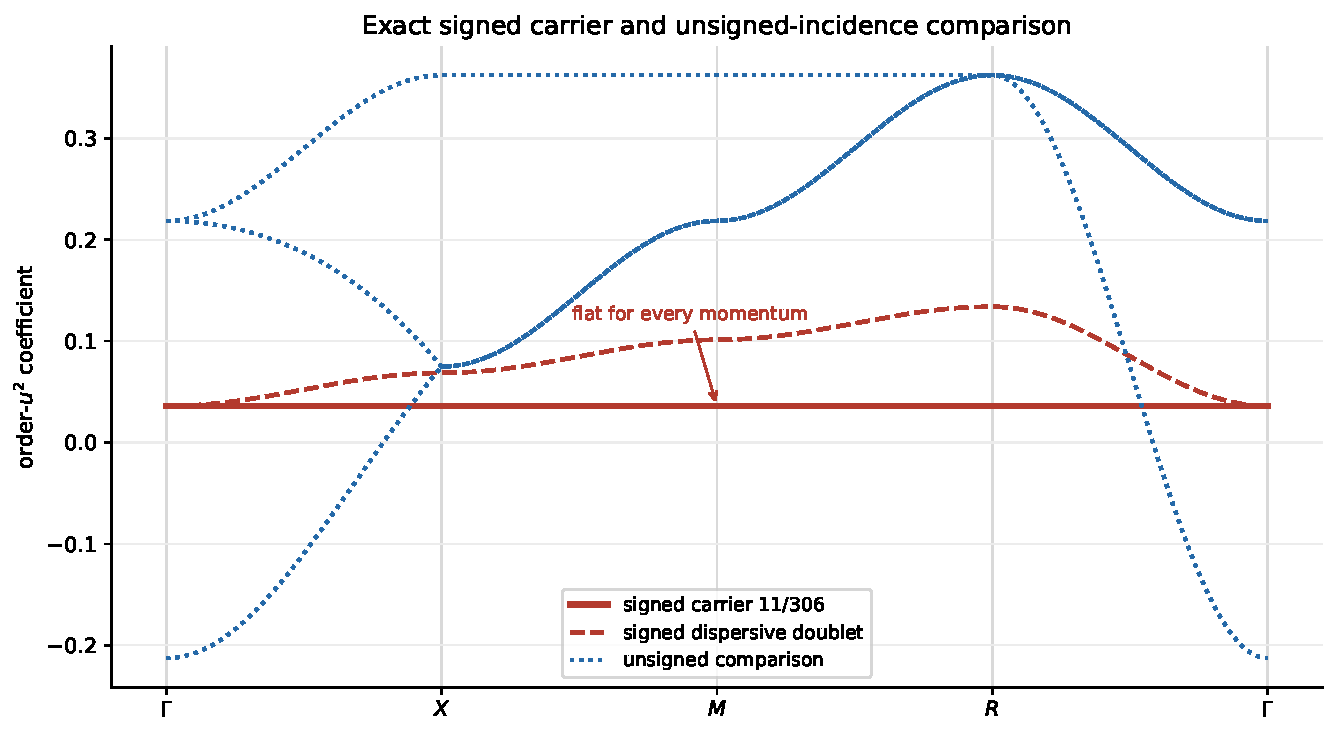
\includegraphics[width=0.94\textwidth]{figure_second_order_bands.pdf}
\caption{Order-$u^2$ coefficients along
$\Gamma$--$X$--$M$--$R$--$\Gamma$. The red carrier and dispersive doublet
are the signed incidence result; their global assembly is
Corollary~\ref{cor:assembly}. The blue curves are the charge-even
second-order bands $d^+_{2,3}+\ell_3(\lambda-4)$ of
Theorem~\ref{thm:even-symbol}, $\lambda$ running over the unsigned spectrum.}
\label{fig:secondorder}
\end{figure}

\subsection{The orientation signs are essential}

Removing the orientation signs --- from the entries of \eqref{eq:B} and from
the phases, so each $e^{ik}-1$ becomes $e^{ik}+1$ --- gives an unsigned
incidence $\mathcal N(k)$. Define its comparison adjacency by
$A_+(k):=\mathcal N(k)\mathcal N(k)\dg-4I$.
Its adjacency spectra at $\Gamma$ and $R$ are $\{12,0,0\}$ and $\{-4,-4,-4\}$,
which share no eigenvalue, so no level can be momentum independent. The flat
branch is therefore not a generic consequence of three face orbitals or cubic
symmetry.

Section~\ref{sec:even} computes the unsigned comparison spectrum in closed
form. The signed span is $8-(-4)=12$, giving the charge-odd second-order width
$12t_3=5/51$ at $N=3$. The unsigned continuous-zone span is
$12-(-4)=16$. By Theorem~\ref{thm:even-symbol}, $16|\ell_3|=88/153$ is the
charge-even second-order bandwidth for even $L$, and coefficientwise as
$L\to\infty$; on a finite torus the value $-4$ is sampled only when $L$ is
even.
\chk{the two band spans ARE the two incidence spectra}

\section{The second-order coefficient on a two-cube space}
\label{sec:twocube}

Everything above derives $t_N$ from a resolvent ledger indexed by the fusion
channel of one shared link. That ledger is representation theory carried out on
a single plaquette pair; it has never been tested against an operator
calculation on a space large enough for two cubes to interact. This section
reports such a test and, more importantly, states what it settles.

The construction is the open face-sharing $(3,2,2)$ prism with its eleven
oriented plaquettes, in the exact-Casimir $\mathcal B=6$ $SU(3)$ truncation, of
basis dimension $1{,}590{,}462$. The delivery reports that it reaches the
relevant sector through $794$ paths and $398$ reachable states; it does not
assemble a $1{,}590{,}462$-dimensional magnetic matrix. Its complete
charge-odd one-plaquette shell at
$E_*=8/3$ has dimension eleven --- a census result and not the plaquette count.
The full $E_*$ eigenspace has dimension $22$, split $11_{C=+}\oplus11_{C=-}$ by
tensor-derived charge conjugation, and the delivery removes all $22$ from the
pseudoinverse; because the eleven columns exhaust the odd half, that agrees
with the $Q=1_--P_-$ prescription of \eqref{eq:heff}. Writing $K_{LR}$ for the raw second-order
operator and $K_L,K_R,K_F$ for the left-cube, right-cube and shared-face
operators in their own coordinates, the connected operator is defined by the
literal M\"obius fold
\begin{equation}\label{eq:mobius}
  K_{\mathrm{conn}}=K_{LR}-J_LK_LJ_L\dg-J_RK_RJ_R\dg+J_FK_FJ_F\dg ,
\end{equation}
and the same fold applied to the geometry gives $G_{\mathrm{conn}}$. The fold
is literal in the sense that no eigenvalue or fitted scalar is subtracted: each
source operator is folded in its own coordinates and lifted. The delivery
corroborates that internally by applying the same weights history by history
over its $1{,}984$ ordered two-step histories, of which $1{,}192$ cancel at
weight zero, and the two routes agree to $4.9\times10^{-15}$.

First order settles itself. Equation~\eqref{eq:su3-same-face-Q} gives
$PVP=-I_{11}$ on the $SU(3)$ charge-odd shell, so the first-order Hamiltonian
coefficient is $H_1=-PVP=+I_{11}$. It shifts all eleven branches equally and
creates no branch ambiguity. Its connected fold then vanishes
\emph{identically}, and by
counting rather than by cancellation --- each of the eleven faces is covered
exactly once by $\{L,R\}$ once the shared face is restored by $F$, so every
M\"obius weight in \eqref{eq:mobius} applied to the identity is $1-1=0$.
Second order is therefore the leading connected term and not a correction to a
first-order one.
\chk{connected first order vanishes by inclusion-exclusion, not by cancellation of numbers}

At second order the result is
\begin{equation}\label{eq:kconn}
  K^{(2)}_{\mathrm{conn}}=\frac{5}{612}\,G_{\mathrm{conn}}+D ,
\end{equation}
with $D$ diagonal and delivered. The geometry alone fixes the \emph{splitting}
inside each block and nothing else: $G_{\mathrm{conn}}$ turns out to be four
disjoint $2\times2$ blocks plus three isolated directions
(Appendix~\ref{app:twocube}), so each pair splits by $2\times5/612=5/306$ about
its own diagonal entry. Given $D$, which Appendix~\ref{app:twocube} prints,
  the spectrum is then closed form: $0$ once, $-\tfrac{15}4$ twice,
  $-\tfrac{34}9$ four times, and $-\tfrac{129}{34}$ four times ---
exact arithmetic on entries that are themselves reconstructions, a boundary
made precise below.
The delivery reports the coefficient recovered target-blind --- supplied to no
builder, graph fit, branching rule or validator --- and reports that the payload
hashes were produced before the recorded comparison, a chronology it itself
calls record-backed and only partly auditable; the value is byte-present in the
nested $\mathcal B=4$ package that the $\mathcal B=6$ build seals as an authority object, so the
defensible statement is dependency-path nonuse and not corpus-wide absence.
This paper re-thresholds those delivered gates rather
than re-running the build, including a deliberately wrong-sign control that the
held-out scaling rejects: on a $66$-dimensional held-out word space the correct
second-order residual falls with log-log slope $2.90$ while the sign-reversed
control falls with slope $2.00$, a minimum error ratio of $325$. What all this
establishes is runtime nonuse of the comparator on the delivered dependency
path, which is not a preregistration. The finite-$u$ validations are
asymmetric: the $\mathcal B=4$ delivery reports a direct diagonalisation of
the full $4{,}180$-dimensional charge-odd space at four small nonzero
couplings, two held out. After subtracting
$E_*+u+u^2\operatorname{eig}K_{\mathrm{eff}}^{(2)}$, the observed residuals
are reported as consistent with a leading cubic term on that fixed geometry;
the delivery supplies neither an exact $[u^3]$ coefficient nor an analytic
third-order remainder bound. The $\mathcal B=6$ check is restricted to the
$66$-dimensional $P+Q_1$ star.
\chk{the connected two-cube geometry has exactly four cross-cell pairs, each -1}
\chk{the B=6 connected kernel is (5/612) G\_conn + diag, with the certified spectrum}
\chk{the certificate's own gates pass, target-blind, with the wrong-sign control rejected}

Resolving \eqref{eq:kconn} by the irreducible representation the shared link
actually carries in the ranked intermediate state gives six coefficients rather
than four, because a link distinguishes $\rho$ from $\bar\rho$:
\begin{equation}\label{eq:census}
\begin{array}{c|cccccc}
 \rho & \mathbf1 & \mathbf3 & \bar{\mathbf3} & \mathbf6 & \bar{\mathbf6} & \mathbf8\\
 \hline
 c_\rho & \tfrac1{12} & -\tfrac1{12} & -\tfrac1{12}
        & -\tfrac19 & -\tfrac19 & \tfrac{16}{51}
\end{array}
\end{equation}
\chk{the B=6 six-channel census sums to the registry's own t\_3 = 5/612}

That these six sum to $5/612$ is weak evidence: six rationals reach one target
in many ways, and a fitted set would pass it. The statement worth making is
stronger, and it is what makes this more than a coincidence of one sum. First,
though, the boundary.

The six coefficients of \eqref{eq:census} are not symbolic: the delivery
stores them as rational reconstructions of pinned finite-precision
Clebsch--Gordan contractions, with a maximum reconstruction residual of
$2.2\times10^{-15}$ per channel --- $2.1\times10^{-14}$ across the delivery's
reconstructed matrices as a whole --- and its own certificate declaring
\texttt{symbolic\_exact\_local\_amplitudes: false}. What follows is therefore
reported, conditional on those six numbers, and not a symbolic identity in the
sense of Theorem~\ref{thm:weingarten}.

\begin{reported}[The census is the Weingarten ledger]\label{rep:census}
At $N=3$ the six reconstructed link-irrep coefficients of \eqref{eq:census}
are the four fusion-channel weights \eqref{eq:w} individually:
\[
  c_{\mathbf 1}=-w_{\mathbf 1},\qquad
  c_{\mathbf 8}=-w_{\mathrm{Adj}},
\]
\[
  c_{\mathbf 3}=c_{\bar{\mathbf 3}}=\tfrac12 w_{\Lambda^2F},\qquad
  c_{\mathbf 6}=c_{\bar{\mathbf 6}}=\tfrac12 w_{\mathrm{Sym}^2F}.
\]
\end{reported}

\noindent Substituting \eqref{eq:table} into \eqref{eq:w} at $N=3$ gives
$w_{\mathbf 1}=-1/12$, $w_{\mathrm{Adj}}=-16/51$, $w_{\Lambda^2F}=-1/6$ and
$w_{\mathrm{Sym}^2F}=-2/9$; comparison with \eqref{eq:census} is then
arithmetic. Six reconstructed rationals landing on four predicted ones, with
the two coincidences the correspondence requires, is a strong consistency
statement and not a proof that the underlying contraction is exact.
\chk{the B=6 six-channel census IS the Weingarten four-channel ledger, channel by channel}

One further feature of the census is worth separating out, because it is the
paper's central architecture measured rather than assumed. The six
link-resolved matrices are not merely six numbers that sum correctly: each is
\emph{separately} proportional to the same incidence Gram. The eleven oriented
plaquettes of the prism have exactly $56$ ordered adjacent pairs, each sharing
one link with signed overlap $\pm1$; the delivery reports a constant
channel-to-geometry ratio on all $56$ of them, for every one of the six
channels, with worst residual $2.2\times10^{-15}$. Colour dynamics fixes a
number per channel and the cellular boundary operator fixes the matrix; if the
two mixed, the ratio would be constant for the total and not for the parts.
\chk{every shared-link channel is separately proportional to the geometry, on all 56 pairs}

The correspondence is scoped to what the Casimir closure exhausts: adjacent,
one-action, shared-link intermediates at order $u^2$. Same-face diagonal
routes, on-site terms and higher-action intermediates lie outside it --- the
$\mathcal B=6$ scalar below is exactly a place where one of them is missing --- and so
does any untruncated-Hilbert-space statement.

It is scoped in one further way, which matters more. The two-cube build draws
its local Wilson amplitudes from the same hash-pinned upstream
Clebsch--Gordan archive as the single-cube reconstructions of the next
subsection, and the squared amplitudes that archive produces are the published
$d_\rho/N^2$~\cite{CBB2025} --- the numerator of \eqref{eq:w}. The census
therefore does not confirm the weights from an independent source: it tests the
\emph{assembly} that carries them, which is the reachable-channel list, the
resolvent denominators, the operator-level fold, the even split between
conjugates, and the geometry that survives each channel separately. That is the
statement worth making, and it is a different statement from confirmation.

Two features of the correspondence carry the content. The mixed family enters
negated because $t_N=B_N-A_N$, which is the same relative sign the incidence
orientation carries. And each like-family \emph{fusion} weight is split evenly
between the irrep and its conjugate --- the two orientations of the shared link
weighted equally --- which the delivery resolves on the two-cube space and
which the next proposition proves at every rank.

\begin{proposition}[Link-resolved census, all ranks]\label{prop:split}
For every $N\ge3$, resolve the adjacent charge-odd cross element of
Theorem~\ref{thm:allrank} by the orientation monomial that places
$F\otimes F$ or $\bar F\otimes\bar F$ on the shared link, that is by the irrep
$\rho$ or $\bar\rho$ the link carries in the intermediate state. Then
$c_{\mathbf1}=-w_{\mathbf1}$ and $c_{\mathrm{Adj}}=-w_{\mathrm{Adj}}$ on the
self-conjugate mixed channels, and the two like monomials carry
$c_\rho=c_{\bar\rho}=\tfrac12w_\rho$ each for
$\rho\in\{\Lambda^2F,\mathrm{Sym}^2F\}$, the six summing to $t_N$. For $N\ne4$
the two like labels are distinct and this is the link-resolved split; at
$N=4$, where $\Lambda^2F$ is self-conjugate, its two monomials land on one
label and a census keyed by the irrep shows the single entry
$w_{\Lambda^2F}$.
\end{proposition}

\begin{proof}
In the orientation table \eqref{eq:orientation-channel-table} the like family
is reached by exactly the two monomials with $\epsilon\epsilon'=ss'$ ---
$(\epsilon,\epsilon')=(+,+)$ and $(-,-)$ when $ss'=1$, the other two when
$ss'=-1$ --- each with coefficient $\epsilon\epsilon'/2=ss'/2$, the
orientation factor $ss'$ that $c_\rho$ multiplies in the cross element; the
first puts $F\otimes F$ on the shared link and the second
$\bar F\otimes\bar F$, that is $\rho$ and $\bar\rho$, with the same weight
$d_\rho/N^2$ because Haar measure is conjugation invariant. The mixed
channels are self-conjugate; they are reached by the two monomials with
$\epsilon\epsilon'=-ss'$, coefficient $-ss'/2$ each, adding to the table's
$\eta_\rho ss'$ with $\eta_\rho=-1$. Charge conjugation commutes with $H_E$, with $V$ and with any
link-Casimir cutoff, so the statement holds under every such truncation.
\end{proof}
\chk{the link-resolved census split is a theorem at every rank: -w\_rho on the self-conjugate mixed channels, w\_rho/2 on each like channel and its conjugate}

\noindent Revision 5 stated this as a conjecture and named a link-resolved
census at $N\ge4$ as its falsifier. No census is needed: the split is the
bookkeeping of the shared-link theorem, and the delivered $N=3$ census
\eqref{eq:census} is a test of the delivery against it, which it passes
channel by channel \leanref{census\_three}.

\subsection{One truncation, two constructions}

The two-cube space also isolates why a cutoff can reverse the sign of $t_3$.
An adjacent shared-link channel $\rho$ is reachable only if the endpoint
Casimir budget $C_2(\rho)+2C_2(\mathbf 3)$ fits inside the truncation: the
sextet needs exactly $6$ and the adjoint $17/3$, so both survive
$\mathcal B=6$ and neither survives $\mathcal B=4$.
\chk{B=6 retains every adjacent shared-link channel; B=4 provably cannot}

\begin{corollary}[What a link cutoff drops]\label{cor:cutoff}
Retaining only the singlet and $\Lambda^2F$ routes projects the second-order
hopping to
\[
  w_{\Lambda^2F}-w_{\mathbf 1}=-\tfrac1{12},
\]
opposite in sign to $t_3$ and $10.2$ times larger in magnitude. What is
dropped is
\[
  w_{\mathrm{Sym}^2F}-w_{\mathrm{Adj}}=\tfrac{14}{153},
\]
and $-\tfrac1{12}+\tfrac{14}{153}=\tfrac5{612}=t_3$. This is arithmetic on
\eqref{eq:w} alone.
\end{corollary}

\noindent The published $p+q\le1$ link cutoff retains exactly those two
routes --- a per-link restriction, where $\mathcal B=4$ is a total endpoint
budget, so the two schemes agree on the retained channels at this order and are
not the same rule --- so $-1/12$ is its projected adjacent hopping and
$14/153$ is the adjacent-hopping correction that completes it --- not
$5/612$, which would double-count what it already carries. On the two-cube
space the first of those two numbers is delivered rather than inferred: a
separately sealed $\mathcal B=4$ run on the identical geometry gives
$K^{(2),\,\mathcal B=4}_{\mathrm{conn}}=-\tfrac1{12}G_{\mathrm{conn}}+D_{\mathcal B=4}$
outright, and the Casimir budgets of the previous paragraph say without
reference to any census that $\mathcal B=4$ can reach only
$\{\mathbf1,\mathbf3,\bar{\mathbf3}\}$. Conditional on \eqref{eq:census}, the
same split of the census reproduces it,
$c_{\mathbf 1}+c_{\mathbf 3}+c_{\bar{\mathbf 3}}=-1/12$, and gives the omitted
half as $c_{\mathbf 6}+c_{\bar{\mathbf 6}}+c_{\mathbf 8}=14/153$.
\chk{the B=6 six-channel census IS the Weingarten four-channel ledger, channel by channel}
\chk{FINDING: the T1 link cutoff reverses the sign of t\_3, and 14/153 is what it omits}

\begin{remark}
Two single-cube reconstructions bracket the same statement. A full $\mathcal B=4$ open
cube assembled from the pinned \texttt{ymcirc} $d=3$, $\mathcal B=4$ plaquette data
~\cite{Balaji2026,ymcirc2026} reproduces $-1/12$ and the truncated shell ordering to
$4.3\times10^{-11}$; a $\mathcal B=6$ cube reproduces $+5/612$ and the inverse ordering
to $8.4\times10^{-15}$. Both locate the missing weight at the same $14/153$.

Neither is an independent replication. Both read tabulated plaquette matrix
elements of the same lineage --- and the two-cube build draws its
Clebsch--Gordan amplitudes from the same hash-pinned \texttt{pyclebsch} archive
as the $\mathcal B=6$ cube, so that agreement is a cross-check of assembly and not of
the amplitudes. The published closed form~\cite{CBB2025} is
$d_\rho/N^2$ --- the very numerator of \eqref{eq:w}. This is a cross-check of
assembly, not a third confirmation of $t_3$; the exact rational identity is
Corollary~\ref{cor:cutoff}, which needs no tolerance. The $p+q\le1$
nomenclature and the finite-rank matrix element are both from~\cite{CBB2025},
and single-cube $SU(N)$ diagonalisation in this style goes back
to~\cite{CM2003}.

The correction to the adjacent-hopping coefficient of a published $T_1$
Hamiltonian is therefore $14/153$ and not $5/612$, which would double-count
the two routes $T_1$ already carries. One coincidence of value is worth naming:
$-1/12$ is also the singlet weight $w_{\mathbf 1}$, and the cutoff value is a
\emph{difference} of two weights, not a weight.
\chk{FINDING: a full T1 = B = 4 cube Hamiltonian reproduces -1/12 and the reversed shell}
\chk{FINDING: the B = 6 cube flips the sign back to +5/612, closing the decisive test}
\end{remark}

The $\mathcal B=6$ cube is channel-complete for the hopping and \emph{not} for the
scalar: its scalar is $39/68$ against the bridge's $11/34$, differing by
exactly $1/4$, the local same-face sextet route, which first enters at cutoff
$20/3$ --- integer label $\mathcal B=7$, so any cutoff above $20/3$ already carries it.
\chk{the B = 6 scalar misses the bridge's by exactly the same-face sextet route}

\subsection{What the cutoff moves, and where}

The connected diagonal $D$ is eleven numbers in both deliveries and is treated
as a remainder in both. It is not eleven numbers. The open prism has a symmetry
group --- the cell exchange $x\mapsto2-x$, the two transverse reflections and
the $y\leftrightarrow z$ swap, of order $16$ --- and $D$ is constant on its
orbits, which are $8+2+1$: the eight side faces, the two end caps, the shared
face.

\begin{proposition}[Where the truncation lives]\label{prop:orbit}
The eight-element orbit is exactly the support of the four cross-cell pairs,
and it is the only orbit whose diagonal value differs between the two
truncations: the end caps carry $-15/4$ and the shared face $0$ at both
$\mathcal B=4$ and $\mathcal B=6$, while the side value moves from $-7/4$ to
$-2317/612$. Together with
the four cross-cell blocks carrying the whole off-diagonal change, the entire
$\mathcal B=4\to\mathcal B=6$ difference is confined to the faces that carry connected transport.
\end{proposition}
\chk{the connected diagonal is orbit-constant, and only the transporting orbit moves}

This also says what the nonuniform $D$ is. Where the faces of a complex form a
\emph{single} orbit --- the closed cube of the next subsection, or the periodic
torus under Corollary~\ref{cor:assembly} --- orbit-constancy forces the diagonal to
be scalar, and the operator is exactly $\alpha I+tG$. The prism has three
orbits because it has a boundary. $D$ is the open boundary showing up in the
diagonal, not a failure of the incidence form.

\subsection{The one-cube shell, and why its flat level cannot move}

Those two single-cube reconstructions are usually read as numerical
cross-checks. They are more than that, because the object they diagonalise is
the same chain complex. The six faces of a cube are a closed surface, so in the
outward orientation $\ker\partial_2$ is one-dimensional and spanned by the sum
of all six --- the fundamental class, $b_2(S^2)=1$. That is
Theorem~\ref{thm:carrier} on a complex with no three-cells, where the $L^3-1$
boundaries are absent and only the class survives.

\begin{proposition}[One-cube shell]\label{prop:cube}
On the closed cube surface $G=\partial_2^{\mathsf T}\partial_2$ commutes with
all $24$ proper rotations. The combinations $b_{+i}-b_{-i}$ carry the defining
vector representation and the combinations $b_{+i}+b_{-i}$ the permutation
representation of the three unordered axes, so with the charge-odd inversion
$Pb_{+i}=-b_{-i}$ the shell is
\[
  A_1^{--}\oplus T_1^{+-}\oplus E^{--},
\]
with $G$-eigenvalues $0$, $4$, $6$ and multiplicities $1$, $3$, $2$.
Consequently $\alpha I+tG$ has levels $\alpha$, $\alpha+4t$, $\alpha+6t$.
\end{proposition}

\begin{proof}
The rotations permute the six outward faces, and $G$ is built from the boundary
map, so it commutes with the permutation action. On the antisymmetric
combinations that action is the defining representation by inspection --- $b_{+i}-b_{-i}$
transforms as $e_i$ --- and on the symmetric combinations it is the
permutation representation of $\{\pm e_i\}$, which is $A_1\oplus E$. Under
$Pb_{+i}=-b_{-i}$ the antisymmetric sector is parity even and the symmetric one
parity odd. In these sectors $G$ is $4I$ and $4I-2(J-I)$ respectively, of
spectra $\{4,4,4\}$ and $\{0,6,6\}$; since the three isotypic components have
distinct dimensions the eigenvalues attach to them uniquely.
\end{proof}
\chk{the one-cube shell is A1 + T1 + E, and its flat level is the S\^{}2 fundamental class}

Three things follow. The cubic labels are derived here rather than assigned:
both deliveries assert them and neither builds the symmetry matrices. The
$A_1^{--}$ level is Proposition~\ref{prop:rigid}'s mechanism on a second
complex --- $Gw=0$ there, so that level sits at $\alpha$ for every $t$, and no truncation, no
channel and no coefficient in dispute anywhere in this paper can move it. And
the reversal the two runs report is therefore a statement about the sign of one
number rather than about the shell as a whole: at $\mathcal B=6$ the levels are
$\{39/68,\,371/612,\,127/204\}$ and at $\mathcal B=4$ $\{37/12,\,11/4,\,31/12\}$, in
the opposite order, with $A_1^{--}$ in each case sitting exactly at the scalar.
The relative shell $\{0,4t,6t\}$ is $\{0,\,5/153,\,5/102\}$ at $\mathcal B=6$.

The finite-volume fingerprint of the 28 August finite-$N$ bridge certificate
--- a different release, and named here because a reader tracing it to the
two-cube one would find nothing --- is worth recording
because its most discriminating multiplicity is not a feature of the
truncation: on the periodic $3^3$ torus the incidence eigenvalues $0,3,6,9$
have multiplicities $29,12,24,16$, respectively, and $29=L^3+2$ is
Theorem~\ref{thm:carrier}.
\chk{the certificate's finite-volume fingerprints, and 29 = L\^{}3 + 2 is the Lean cycle count}

\begin{remark}[Scope of the second-order delivery]
Everything above in this section is second order in $u$, finite volume,
strong coupling and charge odd. It bears on $t_N$ and decides nothing about the
fourth-order coefficient of Section~\ref{sec:fourth}. The
$\mathcal B=6$ two-cube construction was not re-run here: its arithmetic is
audited against geometry rebuilt independently, and its diagonal $D$ is
$B$-truncated and not proved cutoff-stable. The older held-out finite-$u$
validation that rejects the wrong-sign control is a $66$-dimensional $P+Q_1$
word space with the $Q_1$--$Q_1$ magnetic block set to zero; it is not the
radius-two $K_{2,\star}$ operator defined below. The two branches are not equally
covered: at $\mathcal B=4$ the delivery reports a direct diagonalisation of
the complete $4{,}180$-dimensional charge-odd block at four small couplings,
two of them held out.  The residual after
$E_*+u+u^2\operatorname{eig}K_{\mathrm{eff}}^{(2)}$ was described by the
delivery as consistent with a leading cubic term; no exact $[u^3]$
coefficient or analytic remainder estimate is certified. At $\mathcal B=6$
no such diagonalisation exists and the $66$-dimensional star stands in for
it. That $\mathcal B=4$ report carries no check here --- its certificate
did not travel --- and is recorded as the delivery's rather than as this
paper's. No external group has reproduced that release. The later radius-two
release is a distinct construction. It neither upgrades the $\mathcal B=6$
cutoff-stability claim nor supplies a radius-three test.
\end{remark}

\subsection{A detached-replayed radius-two Ritz extension}
\label{subsec:radius2}

A later release on the same open $(3,2,2)$ prism supplies charge-odd
cumulative dimensions
\[
  \dim P,\ \dim(P+Q_1),\ \dim(P+Q_1+Q_2)=11,\ 77,\ 773
\]
and charge-even dimensions $1,2,9$. The release calls this construction
cutoff-free: here that means no $\mathcal B$ cutoff inside the declared one-
and two-action frontiers. The radius-two projection itself remains a
truncation of the gauge-theory Hilbert space.

To keep action radius distinct from perturbative order, write the three nested
matrices as $\mathsf K_1$, $\mathsf K_{2,\star}$ and
$\mathsf K_{2,\mathrm{full}}$. In $P+Q_1+Q_2$ block order,
\begin{equation}\label{eq:radius2blocks}
 H_0=\operatorname{diag}(E_sI,H_1,H_2),\qquad
 V=\begin{pmatrix}
 A_0&B&0\\ B\dg&G&C\\ 0&C\dg&D_2
 \end{pmatrix}.
\end{equation}
Here $E_s=8/3$ in the odd seed and $E_s=0$ in the even seed. The three
finite-coupling operators use $K(u)=H_0+uV=E-uM$, $V=-M$, $u=g^{-4}$:
\begin{align}
 \mathsf K_1(u)&=(H_0+uV)|_{P+Q_1},\nonumber\\
 \mathsf K_{2,\star}(u)&=H_0+u\bigl[V\text{ with only }D_2=Q_2VQ_2
 \text{ set to zero}\bigr],\label{eq:k2nested}\\
 \mathsf K_{2,\mathrm{full}}(u)&=(H_0+uV)|_{P+Q_1+Q_2}.\nonumber
\end{align}
Thus ``full'' means complete only within the retained $Q_2$ block.

\begin{proposition}[Onset of the nested-radius differences]
\label{prop:radiusonset}
Let $R_i=(E_sI-H_i)^{-1}$. If $PVQ_2=0$, the leading seed-space operator
present in $\mathsf K_{2,\star}-\mathsf K_1$ is
\begin{equation}\label{eq:radiusincrements}
 \mathcal I_4=BR_1CR_2C\dg R_1B\dg,
 \qquad
 \mathcal I_5=BR_1CR_2D_2R_2C\dg R_1B\dg,
\end{equation}
where $\mathcal I_5$ is the leading term present in
$\mathsf K_{2,\mathrm{full}}-\mathsf K_{2,\star}$.
\end{proposition}

\begin{proof}
Any contribution that enters $Q_2$ must follow the shortest closed block walk
$P\to Q_1\to Q_2\to Q_1\to P$, which contains four insertions of $V$.
Distinguishing the full operator from the star operator additionally requires
one insertion of $D_2$, hence five insertions. The blocks $A_0$ and $G$ may
dress these walks but cannot shorten them. Evaluating the intermediate
resolvents at the seed energy gives \eqref{eq:radiusincrements}.
\end{proof}

The proposition is exact conditional on the declared frontier and sealed block
structure. The following values are direct floating-point evaluations of its
closed products, not exact rationals and not eigenvalue extrapolations.

\begin{reported}[Detached radius-two replay]\label{rep:radius2}
The lowest eigenvalue of the odd second-order seed operator is isolated by
$0.08438094122012973$; the even seed is one-dimensional. Projection of
\eqref{eq:radiusincrements} gives
\begin{center}
\begin{tabular}{@{}lrrr@{}}
\toprule
 & $C=-$ & $C=+$ & odd--even gap\\
\midrule
$\mathcal I_4$ & $-25.63495194947556$ & $-24.807728943850304$
               & $-0.8272230056252567$\\
$\mathcal I_5$ & $-4.933069330883140$ & $-9.116955631684514$
               & $\phantom{-}4.183886300801373$\\
\bottomrule
\end{tabular}
\end{center}
The last entry is the leading $\mathsf K_{2,\mathrm{full}}-
\mathsf K_{2,\star}$ contribution to the retained odd--even gap. It is not the
complete fifth-order coefficient of either unablated sector Hamiltonian. The
weak-$u$ cubic intercept $4.183884987168061$ differs by
$1.31\times10^{-6}$; the direct product, not that fit, defines the reported
coefficient.
\end{reported}

\begin{figure}[ht]
\centering
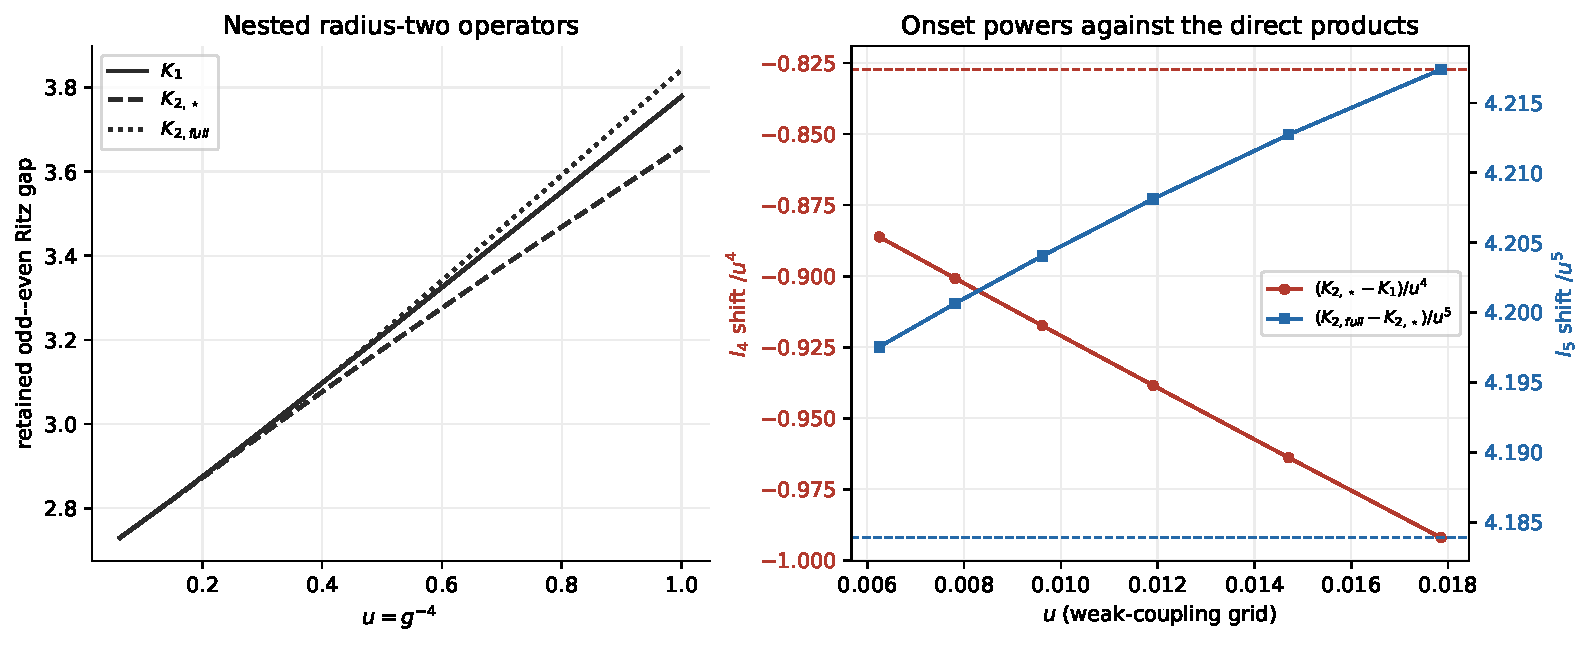
\includegraphics[width=0.98\textwidth]{figure_radius_two_spectrum.pdf}
\caption{Nested radius-two finite-$u$ evidence. Left: retained odd--even Ritz
gaps for \eqref{eq:k2nested}. Right: Hellmann--Feynman path-integral shifts
divided by their predicted onset powers; dashed lines are the direct products
in Reported result~\ref{rep:radius2}. These are retained-space trajectories,
not convergence bands or full-Hilbert-space error estimates.}
\label{fig:radius2}
\end{figure}

The hash-pinned detached verifier starts from both sealed parity-sector parent
operators and recomputes the two coupling grids, all three nested spectra,
residuals, interlacing, direct products, rephasing and adaptive path integrals.
It returned zero maximum recomputation error and maximum rephasing discrepancy
$4.09\times10^{-14}$; all $24$ hostile, algebra, numerical-safety and
serialization tests passed. This is an independent downstream replay of the
sealed parents, not an independent derivation of their microscopic
gauge-basis contractions.

The boundary is quantitative. No odd $Q_3$ matrix is present, so no matched
radius-two error enclosure or convergence claim exists. At $g=1$ the odd and
even ground seed weights have fallen to $0.274$ and $0.277$, while the even
exterior residual is $3.784$; the retained eigenvalues are still accurately
computed, but their accuracy as approximations to a larger space is
uncontrolled there. Nor can an open prism determine the periodic off-axis
fourth-order shape of Section~\ref{sec:fourth}: $\mathcal I_4$ and
$\mathcal I_5$ in \eqref{eq:radiusincrements} do not choose a value of
$C_{\mathrm{shp}}$.

\section{The charge-even sector and the unsigned incidence}
\label{sec:even}

The unsigned incidence $\mathcal N(k)$ of Section~\ref{sec:second} defines an
exact algebraic operator $G_+(k)=\mathcal N(k)\mathcal N(k)\dg$. At order
$u^2$ its identification with the complete linked charge-even effective
Hamiltonian is Theorem~\ref{thm:even-symbol}: the all-pairs vacuum route of
Proposition~\ref{prop:vacuum} is cancelled on every link-disjoint pair, and
the adjacent element is $\ell_N$ whatever the orientations. At order $u^3$ the
identification remains a hypothesis
(Conditional corollary~\ref{prop:evengamma3}), because the third-order
charge-even
coefficients come from the supplied domino ledger and no third-order process
census has been carried out here. With that boundary explicit, write
\[
  \hat a_m=2+2\cos k_m=|1+e^{ik_m}|^2,\qquad p=\sum_m \hat a_m .
\]
The hat is not decoration: $\hat a_m$ is the \emph{complement} of the
$a_m=4\sin^2(k_m/2)$ used in the charge-odd shape basis \eqref{eq:shapes}
below,
$\hat a_m+a_m=4$, and that complementarity is the sum rule below.

\begin{theorem}[Unsigned-incidence Bloch cubic]\label{thm:evencubic}
$p+q=12$ pointwise, and the characteristic polynomial of
$\mathcal N\mathcal N\dg$ is
\[
  \mu^3-2p\,\mu^2+p^2\mu-4\hat a_1\hat a_2\hat a_3
  \;=\;\mu(\mu-p)^2-4\hat a_1\hat a_2\hat a_3 ,
\]
with the unsigned comparison-adjacency eigenvalues $\lambda=\mu-4$. The signed
counterpart of the same computation is $\mu(\mu-q)^2$.
\end{theorem}
\chk{the unsigned-incidence characteristic polynomial is mu(mu - p)\^{}2 = 4 a\_1 a\_2 a\_3}
\chk{p + q = 12: one zone function runs both sectors}

The algebraic closed form is complete rather than merely consistent at sampled momenta:
the characteristic polynomial of the $81\times81$ and $192\times192$ finite
plaquette adjacencies factorises coefficient for coefficient over $\mathbb Z$
into this cubic over the momentum grid.
\chk{the Bloch cubic IS the finite L = 3 and L = 4 plaquette spectrum, exactly}

\begin{proposition}[Range and attainment]\label{prop:evenrange}
$\lambda\in[-4,12]$ exactly. The top $\lambda=12$ is attained only at $\Gamma$
($\hat a_1=\hat a_2=\hat a_3=4$). The bottom $\lambda=-4$ is attained on the
whole of the three planes $k_j=\pi$, where the constant term vanishes, and only
at $R$ is it a triple root.
\end{proposition}

\begin{proof}
Write $f(\mu)=\mu(\mu-p)^2-4\hat a_1\hat a_2\hat a_3$. Then
$f(0)=-4\hat a_1\hat a_2\hat a_3\le0$ and $\mu(\mu-p)^2<0$ for $\mu<0$, so no
root lies below $0$; and $f'(\mu)=(3\mu-p)(\mu-p)>0$ for $\mu>p$, with
$\hat a_1\hat a_2\hat a_3\le(p/3)^3$ by AM--GM and
\[
 f(16)\ge16(16-p)^2-\frac{4p^3}{27}
 =\frac4{27}(12-p)(48-p)^2\ge0.
\]
Hence $\mu\in[0,16]$ and
$\lambda=\mu-4\in[-4,12]$. Equality at the top forces $p=12$ and
$\hat a_1\hat a_2\hat a_3=64$, which is $\Gamma$. Equality at the bottom is
$f(0)=0$, i.e. $\hat a_1\hat a_2\hat a_3=0$, i.e. some $k_j=\pi$; there
$f(\mu)=\mu(\mu-p)^2$ and the root $\mu=0$ is simple unless $p=0$, which is
$R$ alone.
\end{proof}
\chk{the C-even range [-4, 12] is exact; the top only at Gamma, the floor on three planes}
\chk{the C-even band touches its floor exactly on the three planes k\_j = pi}

\begin{remark}
A flat unsigned-comparison branch would need $f(\mu_0)=0$ identically in $k$,
which the constant term already forbids. Its minimum is attained on three
measure-zero planes, against the signed operator's flat band. This contrast is
an exact statement about two incidence constructions; at order $u^2$ the two
constructions are the two physical charge sectors, by
Corollary~\ref{cor:assembly} and Theorem~\ref{thm:even-symbol}. The range
bound itself is proof-checked over the reals: for $a_i\in[0,4]$ the cubic is
strictly negative below $\mu=0$ and strictly positive above $\mu=16$, so
every root lies in $[0,16]$ \leanref{even\_cubic\_neg\_below\_zero},
\leanref{even\_cubic\_pos\_above\_sixteen}.
\chk{the C-even band touches its floor exactly on the three planes k\_j = pi}
\chk{the C-even spectra at the four high-symmetry momenta}
\end{remark}

\subsection{The charge-even assembly, and where it is conditional}

The shared-link coefficient at $r=2$ is all-rank and analytic, and
Theorem~\ref{thm:even-symbol} makes it the charge-even band structure at that
order, with the scalar of Theorem~\ref{thm:scalar-ledger}; nothing at $r=2$
is supplied. The $r=3$ values --- $t_{3,+}=-6335/249696$ and everything
computed from it --- come from the same supplied domino ledger as
Section~\ref{sec:su3}, and are conditional on it in the same way.

The scalar ledger is not a list of separate facts. Writing $\lambda$ for the
adjacency eigenvalue and $\mathrm{tower}_{r,s}$ for the within-plaquette term
in canonical $u$,
\begin{equation}\label{eq:assembly}
  E_s(\lambda,r)=\mathrm{tower}_{r,s}+12\,\mathrm{leak}_{r,s}+\lambda\,t_{r,s},
\end{equation}
with $\lambda\in\{-4,8\}$ in the signed charge-odd sector (carrier and dispersive
top), $\lambda\in\{12,-4\}$ in the unsigned comparison, and $\lambda=0$
returning the on-site diagonals. This reproduces every registered diagonal
and band value --- nine of them --- across both sectors and both orders. The
tower term is the certified coupling conversion $4\Delta(3u/2)$, so
\eqref{eq:assembly} takes no unregistered input. The twelve is a count on this
lattice, not a citation: the plaquette graph is $12$-regular and two distinct
faces share at most one link. The two towers are different objects and both
are needed: the charge-odd one contributes
$8/3+u+u^2/2+7u^3/32$ and the charge-even one $8/3-u+(13/20)u^2+(101/200)u^3$,
each of them $4\Delta(3u/2)$ on its own sector's series, so
$\mathrm{tower}_{2,-}=1/2$ against $\mathrm{tower}_{2,+}=13/20$ and
$\mathrm{tower}_{3,-}=7/32$ against $\mathrm{tower}_{3,+}=101/200$.
\chk{one assembly formula gives every registered band value}
\chk{one assembly formula gives every C-even value at both orders}
\chk{the plaquette graph is 12-regular and two faces share at most one link}

Because the supplied ledger has $\mathrm{leak}_{r,+}=t_{r,+}$ at both computed
orders, the charge-even assembly --- a theorem at $r=2$, conditional at
$r=3$ --- collapses to
$\mathrm{tower}_{r,+}+(12+\lambda)\,t_{r,+}$, a one-parameter family in the
charge-even tower. That
equality is verified and unexplained: at third order the charge-odd leakage
separates from the charge-odd hopping while the charge-even identity survives.
It is recorded as a unifying candidate with a falsifier --- an order at which
the two are computed independently and differ --- not as a mechanism.
\chk{both declared coincidences, checked: one is ell\_N at all ranks, the other is bare}

\subsection{Where the rest frame is not blind}

\begin{proposition}[Charge-even $\Gamma$ splitting at second order]\label{prop:evengamma}
At $\Gamma$ the unsigned spectrum is $\{12,0,0\}$, so by
Theorem~\ref{thm:even-symbol} the $A_1^{++}$ level and the $E^{++}$ doublet
are distinct at every rank $N\ge3$, and
\[
  E(A_1^{++})-E(E^{++})=12\,\ell_N\,u^2+O(u^3),
\]
which is $-\tfrac{22}{51}u^2$ at $N=3$.
\end{proposition}

\begin{conditional}[Third order]\label{prop:evengamma3}
If the unsigned symbol is also the complete linked charge-even symbol at order
$u^3$, the splitting's cubic coefficient is $12t_{3,+}=-6335/20808$.
\end{conditional}
\chk{the C-even Gamma point pins t\_+, exactly where no C-odd Gamma datum can}

This is the structural counterpart of the charge-odd blindness recorded in
Section~\ref{sec:su3}. The signed spectrum at $\Gamma$ is $\{-4,-4,-4\}$, one
level, so no charge-odd rest-frame series can see the hopping; the unsigned
spectrum has two levels, so the charge-even rest frame fixes $\ell_N$ at
second order and, under the third-order symbol hypothesis, $t_{3,+}$. The
$A_1^{++}$
branch is isotropic at leading order without assuming it, with curvature
$\tfrac43|t_{r,+}|$ in all three directions --- $22/459$ at second order and
$6335/187272$ at third.
\chk{the C-even curvature is (4/3)|t\_+| at both orders, and isotropic}

On a finite $L^3$ grid the charge-even width, a theorem at $r=2$ and
conditional at $r=3$, is
\[
 W^{(+)}_{r,L}=|t_{r,+}|\,[12-\lambda_{\min}^{(+)}(L)],
 \qquad \lambda_{\min}^{(+)}(L)=-4\ \Longleftrightarrow\ L\ \text{is even}.
\]
Thus it equals $16|t_{r,+}|$ for even $L$ and approaches that coefficientwise
as $L\to\infty$; the charge-odd manifold width is $12|t_{r,-}|$ for even $L$.
At any order at which the correction
stays in the incidence algebra --- which Proposition~\ref{prop:rigid} warns is
not automatic --- the second-order ratio is $4(3N^2-5)/[3(N^2-4)]$, finite and
greater than one at every rank $N\ge3$, decreasing from $88/15$ at $N=3$
towards $4$ \leanref{width\_ratio\_numerator}. So at second order the
charge-even band is the wider one at every rank --- for even $L$, and
coefficientwise as $L\to\infty$, with no symbol hypothesis --- and that
asymmetry is a channel statement rather than a geometric one.
\chk{the C-even bandwidth is 16|t\_+| at every order; the C-odd manifold width is 12|t\_-|}
\chk{at N = 2 the C-odd hopping vanishes and the C-even one does not}

\section{\texorpdfstring{$SU(3)$}{SU(3)} through third order}
\label{sec:su3}

The \emph{third-order} content of this section is an externally verified
computational input: the frozen upstream corpus reports a $251/251$ cold exact
replay for the retained chain, while this compact release checks only the
assembled rationals. At second order both the hopping $t_3$ and the flat
scalar $11/306$ are analytic: Theorem~\ref{thm:scalar-ledger} gives the tower
$\tfrac12=\sigma^-_3+1/\CF$ and the leakage $\mathrm{leak}_2=\ell_3$, which the
upstream ledger had recorded as an identification. The within-plaquette tower
is $8/3+u+u^2/2+7u^3/32$, its cubic term from the supplied ledger.

\begin{reported}[Third-order ledger]\label{rep:su3}
The supplied ledgers report, in exact rationals,
\[
  b_3=\frac{1975}{124848},\qquad
  \mathrm{leak}_3=-\frac{12331}{249696},
\]
and the assembled flat scalar
$d_3=\tfrac7{32}+12\,\mathrm{leak}_3-4b_3=-\tfrac{109151}{249696}$.
\end{reported}
\chk{d\_3 = 7/32 + 12*leak\_3 - 4*b\_3}
\chk{leak\_3 is assembled from the domino diagonal and the vacuum piece}

\begin{conditional}[Third-order factorisation]\label{cor:su3}
If the lifter census is exhaustive and the linked ledger complete, then
\[
  T_{\le3}H_{\mathrm{eff},-}(k,u)
  =E_{\mathrm{flat}}^{[3]}(u)I+\tau^{[3]}(u)B(k)B(k)\dg,
\]
\[
  \begin{aligned}
    E_{\mathrm{flat}}^{[3]}(u)&=\tfrac83+u+\tfrac{11}{306}u^2-\tfrac{109151}{249696}u^3,\\
    \tau^{[3]}(u)&=\tfrac5{612}u^2+\tfrac{1975}{124848}u^3 .
  \end{aligned}
\]
This is an equality of Taylor coefficients through order three at each fixed
volume; no $L$-uniform fourth-order remainder is claimed.
\end{conditional}
\chk{E\_flat and t(u) carry the ledger coefficients}

The second-order diagonal is the $\lambda=0$ value
$\tfrac12+12\,\mathrm{leak}_2=7/102$ with $\mathrm{leak}_2=-11/306$;
subtracting $4t_3$ gives the flat scalar $11/306$ at $\lambda=-4$. Both are
now Theorem~\ref{thm:scalar-ledger} at $N=3$.
\chk{d\_- = 1/2 + 12*leak\_2, and leak\_2 = -11/306}

\begin{remark}[What the external comparison can and cannot do]
Hamer's 1989 rest-frame series~\cite{Hamer1989} agrees with
$E_{\mathrm{flat}}^{[3]}$ at every shared order. It cannot test
$\tau^{[3]}$. The hopping enters the coefficientwise spectrum only through
$\tau^{[3]}(u)q(k)$ and $q(0)=0$, so every \emph{charge-odd}
$\Gamma$-point datum is blind to it. The charge-even rest frame is not, by
Proposition~\ref{prop:evengamma}; the one-parameter family
$(b_3+\varepsilon,\ \mathrm{leak}_3+\varepsilon/3)$ leaves $d_3$ and therefore
the entire comparison unchanged. What the agreement pins is the combination
$12\,\mathrm{leak}_3-4b_3$. The $\lambda=8$ band top separates them, via \eqref{eq:assembly}.
Proposition~\ref{prop:evengamma} is the charge-\emph{even} analogue and
separates $\mathrm{leak}_+$ from $t_+$; it says nothing about $b_3$ or
$\mathrm{leak}_3$.
\chk{FINDING: no Gamma-point datum can constrain the hopping}
\end{remark}

\section{What the homology protects}

\begin{proposition}[Boundary-factorised rigidity]\label{prop:rigid}
If an order-$r$ Bloch correction has the form
$H_r(k)=a_rI+b_rS(k)+B(k)M_r(k)B(k)\dg$, then for every $k\neq0$,
$H_r(k)w(k)=(a_r-4b_r)w(k)$: the correction shifts the carrier without
dispersing it.
\end{proposition}

\begin{proof}
$B\dg w=0$ and $Sw=-4w$, both from Theorem~\ref{thm:fact}. The middle term is
annihilated whatever $M_r$ is, which is the content: the protection belongs to
the boundary operator and not to the dynamics.
\end{proof}
\chk{a boundary-factorised correction shifts the carrier without dispersing it, for generic M}

In real space this is the orthogonality of the two cellular Laplacians,
$L^{\downarrow}_2L^{\uparrow}_2=L^{\uparrow}_2L^{\downarrow}_2=0$, so any
polynomial in them acts on $\ker L^{\downarrow}_2\cap\ker L^{\uparrow}_2$ by
its constant term. The proposition is not an unconditional all-orders
statement: $\{BMB\dg\}$ is not a two-sided ideal in $\mathrm{End}(C_2)$, and a
general higher-order correction need not factor through links. Cubic symmetry
alone permits carrier-projected fourth-order shapes built from
\begin{equation}\label{eq:shapes}
  1,\quad q,\quad e_2,\quad \frac{4e_2}{q},\quad \frac{e_3}{q},
\end{equation}
with $e_2=\sum_{i<j}a_ia_j$, $e_3=a_1a_2a_3$ and $a_i=4\sin^2(k_i/2)$. The
$1/q$ is the carrier projection: $\|w\|^2=q$ by Theorem~\ref{thm:fact}, so the
carrier-projected correction is $\varepsilon_4=(w\dg H_4w)/q$ and the
numerator, not $\varepsilon_4$, is the polynomial.
\chk{the carrier projection is where the 1/q comes from}
\chk{clearing the denominator reproduces the five-element numerator basis}

\section{The fourth-order boundary}
\label{sec:fourth}

Two supplied fourth-order records agree on the axial datum and on the
appearance of mobility, and disagree on one off-axis mixed-gradient
coefficient $C_{\mathrm{shp}}$. This edition does not adjudicate the
coefficient, and no fourth-order band or bandwidth is used above. What it does
is three things, each checked. It locates the disagreement exactly, as the
weight of the single operator outside the algebra of the two cellular
Laplacians (Section~\ref{sec:hodge-form}). It reports four of the kernel's
amplitudes recomputed reading neither kernel, which decides the
\emph{standing} of the two records without deciding the coefficient, and
puts a third value on record (Section~\ref{sec:outside}). And it keeps the
obstruction theorem, which says why no rest-frame or axial datum can decide
it.

After subtracting the rest value, the recorded carrier ansatz is
\begin{equation}\label{eq:shapeansatz}
 \Delta_4(k):=\varepsilon_4(k)-\varepsilon_4(0)
 =Aq+Be_2+C_{\mathrm{shp}}\frac{4e_2}{q}
   +D\frac{e_3}{q}.
\end{equation}
The continuous $k\to0$ limit is used at $q=0$. Denote the two recorded
mixed-gradient values by $C_{\mathrm{old}}$ and $C_{\mathrm{new}}$ and set
$\Delta_C=C_{\mathrm{new}}-C_{\mathrm{old}}$. A supplied all-rank cube ledger
also reports
\begin{equation}\label{eq:alphaN}
 \alpha_N=\frac{640}{N(N^2-1)^3},
\end{equation}
but this formula and its identification with the complete axial coefficient
remain conditional on that ledger. Sealed packages containing other
fourth-order scalars use incompatible observable labels; none is promoted here
to a canonical rest coefficient.

\subsection{An exact theorem for the saved historical kernel}

The upstream authority corpus supplies the hash-pinned $189$-record historical
kernel. Pulling its centered fourth-order operator back to cube amplitudes with
$\mathsf C=\partial_3$, define
\[
 Q_4=\mathsf C\dg H_4\mathsf C,
 \qquad G=\mathsf C\dg\mathsf C,
 \qquad \mathcal Q_4=Q_4-s_4G,
\]
where $s_4=\operatorname{tr}H_4(\Gamma)/3$. If
$L_i=2I-T_i-T_i^{-1}$, then $G=\sum_iL_i$ and the centered coefficient is the
generalized eigenvalue $\mathcal Q_4\phi=\lambda_4G\phi$. The representative
change $(Q_4,G)\sim(Q_4+\delta G,G)$ is a scalar gauge only when the scalar
anchor changes simultaneously; it cannot change an off-axis shape.

\begin{reported}[Exact saved-kernel Hodge pencil]\label{rep:historical}
For the supplied historical kernel,
\[
 q_{\mathrm{old}}^{(4)}
 =-\frac{20721577909065127111}{7250590288602460800},\qquad
 \alpha_{\mathrm{old}}=\frac5{12},\qquad
 \beta_{\mathrm{old}}
 =\frac{17607806155349}{275331901291200},
\]
and
\begin{equation}\label{eq:oldhodge}
 \mathcal Q_{4,\mathrm{old}}
 =\frac5{48}\sum_iL_i^2
 +\frac{17607806155349}{1101327605164800}
   \sum_{i<j}L_iL_j\succeq0.
\end{equation}
Its continuous-zone and even-$L$ width is
\[
 W_{4,\mathrm{old}}=\alpha_{\mathrm{old}}+\beta_{\mathrm{old}}
 =\frac{132329431693349}{275331901291200}.
\]
These identities are exact for the saved kernel and its cold fixed-kernel
checks. They do not establish that this kernel is the unique physical linked
fourth-order operator.
\end{reported}

The corresponding $25$-point numerator stencil has
\[
 w_0=\tfrac92\alpha+3\beta,\qquad
 w_1=-(\alpha+\beta),\qquad
 w_2=\tfrac14\alpha,\qquad
 w_d=\tfrac14\beta,
\]
and obeys $w_0+6w_1+6w_2+12w_d=0$ exactly. For
$\alpha,\beta>0$, the generalized dispersion is bounded by
$0\le\lambda_4\le\alpha+\beta$, with the continuous-zone extrema at
$\Gamma$ and $R$ respectively; an odd-$L$ grid does not contain $R$.

\begin{figure}[t]
\centering
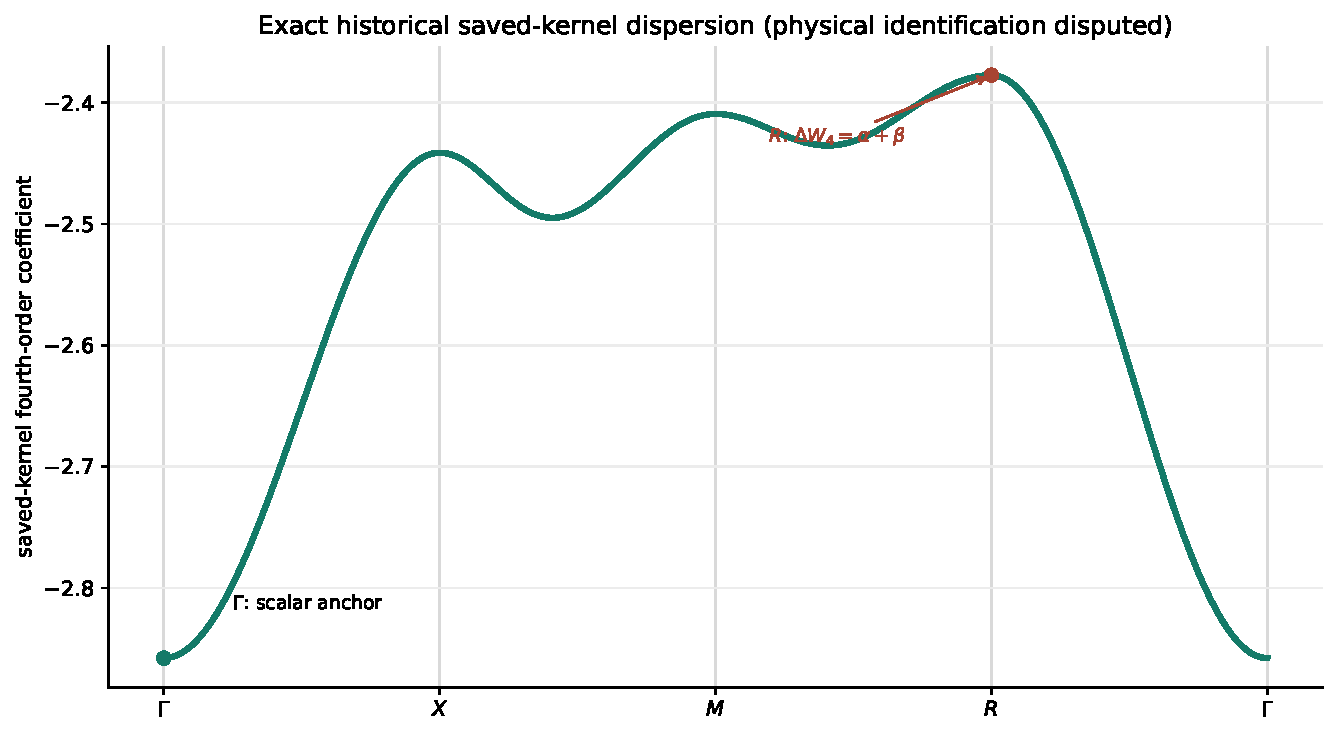
\includegraphics[width=0.94\textwidth]{figure_historical_fourth_order.pdf}
\caption{Exact dispersion of the saved historical kernel in
Reported result~\ref{rep:historical}. The plot is a theorem about that
hash-pinned kernel. Its identification with the complete physical linked
$SU(3)$ fourth-order operator is disputed, so the curve is not used as a
settled physical band.}
\label{fig:historical}
\end{figure}

The two records do agree on the axial datum, but the corpus's own quoted
tolerance does not cover that agreement: the $\alpha$ gap is
$2.43\times10^{-13}$ against a stated bound of $2.3\times10^{-13}$. The sealed core holds internally --- $\alpha_{\mathrm{new}}$ and
$4A_{\mathrm{new}}$ agree to $2\times10^{-15}$ --- which is consistent with the
quoted bound being too tight, but two float comparisons do not discriminate
that from a shared upstream slip. Recorded as a discrepancy rather than
resolved, and the bound is not widened.
\chk{v10a.26 A, B, D match the sealed rationals within 2.3e-13}
\chk{FINDING: alpha\_new falls outside the corpus's own 2.3e-13 bound}

\subsection{The obstruction is polynomial}

\begin{theorem}[Obstruction certificate]\label{thm:obstruction}
The two recorded off-axis coefficients enter \eqref{eq:shapes} only through
the shape $4e_2/q$, so the two records' carrier numerators differ by
$4\Delta_C e_2$ and their bands by $\Delta_C\,(4e_2/q)$. On any
one-dimensional axial cut two of the three $a_i$ vanish, so $e_2$ is the
\emph{zero polynomial} there and both differences vanish identically.
Consequently no $\Gamma$-point or axial datum distinguishes the two records,
at any precision. Off axis they do differ: $e_2(M)=16$ and $e_2(R)=48$, so the
numerators differ by $64\Delta_C$ and $192\Delta_C$ and the bands by
$8\Delta_C$ and $16\Delta_C$.
\end{theorem}
\chk{FINDING: the retained Gamma/axis data cannot identify C\_shp}
\chk{Phi\_C vanishes at Gamma along every direction}

\begin{remark}
The vanishing is polynomial, not numerical: this is non-identifiability, not a
limitation of the data in hand. Re-anchoring cannot substitute, and neither
record is preferred here. An off-axis contraction is the only decider.
\chk{the crosswalk is exactly scalar on the momentum axes}
\end{remark}

On the axial cut itself the invariants collapse to
$q=q_{\mathrm{ax}}(k)=4\sin^2(k/2)$ with $e_2=e_3=0$. Dividing the raw
cube-boundary numerator $(\alpha_N/4)q_{\mathrm{ax}}^2$ by
$\|w\|^2=q=q_{\mathrm{ax}}$ leaves one power of $q_{\mathrm{ax}}$ with
coefficient $\alpha_3/4=5/48$.
\chk{on an axial cut the mixed invariants vanish and the norm divides}

\subsection{A second witness}

Non-identifiability is better exhibited than argued from a difference between
two records, since a difference could always be a computational error in one of
them. The witness below is not itself a candidate for the physical
coefficient. It is the balanced continuation obtained in the supplied source
by setting an auxiliary bookkeeping parameter $\epsilon$ to zero; that source
label carries no physical meaning here. Its sole role is to make the
$4\Delta_Ce_2$ family concrete with an exactly known shift.

\begin{proposition}[Explicit second witness]\label{prop:witness}
There is a value $C_{\mathrm{alt}}$ with
$C_{\mathrm{alt}}-C_{\mathrm{old}}=25/1024$ exactly, appearing verbatim in the
pinned source edition, whose induced band separations are $0$ at $X$,
$25/128$ at $M$ and $25/64$ at $R$. It is identical to
$C_{\mathrm{old}}$ on every retained datum and distinct from it off-axis.
\end{proposition}
\chk{FINDING: an explicit second witness C\_alt exhibits the C2 non-identifiability}
\chk{the C\_alt witness IS the balanced eps-free continuation, and Delta\_C/(A/2) = 15/32}

\subsection{Where the coefficient lives}

The four checkpoint deltas are the $\Gamma$-subtracted carrier corrections
$\Delta_s=\varepsilon_4(k_s)-\varepsilon_4(0)$ at
$k_X=(\pi,0,0)$, $k_M=(\pi,\pi,0)$, $k_P=(\pi,\pi/2,0)$ and
$k_R=(\pi,\pi,\pi)$ --- $P$ is the off-axis, off-corner point that makes the
system invertible, with $a=(4,2,0)$. Its algebraic role is explicit here; no
additional provenance is inferred for that checkpoint. In the shape basis they are
\begin{equation}\label{eq:checkpoints}
\begin{aligned}
  \Delta_X&=4A,\\
  \Delta_M&=8A+16B+8C_{\mathrm{shp}},\\
  \Delta_P&=6A+8B+\tfrac{16}3C_{\mathrm{shp}},\\
  \Delta_R&=12A+48B+16C_{\mathrm{shp}}+\tfrac{16}3D,
\end{aligned}
\end{equation}
and they invert exactly, so the four shape coefficients are recoverable from
four checkpoints. $\Delta_X$ contains $A$ alone, which is why the axial cuts
agree whatever the dispute does.
\chk{checkpoint values at X, M, P, R}
\chk{the four extraction formulas invert the ansatz}
\chk{X is blind to B, C, D — it fixes A alone}

Four further measurements locate the coefficient and bound where a
disagreement could live. The distinction matters and is easy to lose: showing
where a coefficient's \emph{value} is concentrated is not by itself showing
where a \emph{discrepancy} can sit. Only the third item below does the second
thing.

\begin{enumerate}\itemsep2pt
\item \textbf{The shape fit's $C$ row sums to zero}, so no error in the
  $\Gamma$ anchoring can move $C_{\mathrm{shp}}$ at all; the recorded run's own
  re-anchoring moved it by $4.6\times10^{-15}$, as the zero row sum requires.
  A scalar shift is translation-local and changes nothing observable, which is
  why the two anchored scalars $q_{\mathrm{band}}^{(4)}$ and
  $m_\Gamma^{(4)}$ are differently anchored coordinates and not rival
  estimates.
\item \textbf{The coefficient's value is concentrated, not spread.} Six of
  the $189$ kernel records --- the normal $(0,0,1)$ shell --- carry $81\%$ of
  the total weight, while the $120$ rotation records carry $6\%$ and are $255$
  times less sensitive per record. This says where the coefficient lives, not
  yet where the two records can differ.
\item \textbf{The agreed axial coefficient pins the normal sector.} All six
  normal records share one amplitude $h$, and it sets both shapes rigidly:
  $A_{\mathrm{normal}}=-h$ while the raw normal amplitude is $2h$, which in the
  shape normalisation of \eqref{eq:shapes} is $C_{\mathrm{normal}}=h/2$, so
  \[
    C_{\mathrm{normal}}=-\tfrac12 A_{\mathrm{normal}}\quad\text{exactly.}
  \]
  (The factor of four between $2h$ and $h/2$ is the raw-to-shape conversion,
  not a discrepancy.) Granting $A=5/48$ --- which both records share --- together
  with the block decomposition, which puts $5/48+4x$ on the normal block and
  $-4x$ on the mixed one, therefore fixes $h$ and with it $81\%$ of the
  coefficient; and everything free to move without disturbing $A$ totals less
  than half the disputed gap. A rival kernel must differ \emph{structurally} in
  the $A$-carrying sector; no redistribution reaches the gap.
\item \textbf{The two kernels agree almost everywhere.} Their supports are
  identical and $144$ of $189$ records ride one common scale; the divergent
  cross sector is a single uniform ratio. The dispute is three amplitudes.
\end{enumerate}
\chk{the shape fit's C row sums to zero, so no Gamma-anchor error can move C\_shp at all}
\chk{a translation-local scalar shift changes nothing observable}
\chk{FINDING: C\_shp is carried by 6 of 189 records, not spread across the kernel}
\chk{FINDING: A = 5/48 pins the normal sector's whole C4 contribution}
\chk{C\_normal = -A\_normal/2: the agreed axial coefficient pins the normal channel}
\chk{the two 189-record kernels agree everywhere except three amplitudes, and the on-site anchor swap moves C by exactly zero}

Read together these four sharpen the target and prefer no side of it. They say
that a rival kernel must differ structurally in the $A$-carrying sector rather
than by redistribution. That is a constraint on candidates built on the
recorded $189$-record support --- which is where the measurement was made; a
kernel on a different support is not constrained by it at all. Neither record is promoted here and neither is withdrawn: the interval of
\emph{values} between them is not narrowed. What is narrowed is the class of
\emph{kernels} that can reach either end, and that constraint bears on both
records alike.

\subsection{The kernel is a Hodge polynomial plus one operator}\label{sec:hodge-form}

Write $L^\downarrow=\partial_2\dg\partial_2$ and
$L^\uparrow=\partial_3\partial_3\dg$ for the two cellular Laplacians on
plaquettes, $S_\square=L^\downarrow-4I$ for the signed shared-link adjacency of
Theorem~\ref{thm:fact}, and $R$ for the cross-plane half of $S_\square$
(equivalently, minus the cross-plane half of $L^\uparrow$). The $189$-record
historical kernel carries exactly six weight magnitudes, one per cubic orbit
of displacements: the on-site $\sigma$, the normal $\nu$, the in-plane $\pi$,
the two-hop $u$ with its doubled orbit $u_2=2u$, and the rotation $\rho$. Over
the whole zone the shape coefficients are closed form in them,
\begin{equation}\label{eq:orbit-shape}
 A=\tfrac5{48},\qquad B=D=0,\qquad
 C_{\mathrm{shp}}=-\tfrac5{96}-u-\tfrac12(\rho+\pi),
\end{equation}
with $\nu=-(\tfrac5{48}+4u)$ forced by $A$ and $\sigma$ entering the rest
value alone \leanref{nu\_from\_A\_and\_u},
\leanref{C\_shp\_from\_orbits\_historical}.
\chk{the 189 records carry exactly six weight magnitudes}
\chk{the shape coefficients are solved, not fitted: A = 5/48, B = D = 0 exactly}
\chk{C\_shp = -5/96 - u - (rho + pi)/2, exactly}
\chk{A = 5/48 forces the normal amplitude: nu = -(5/48 + 4u)}

\begin{reported}[Hodge normal form of the saved kernel]\label{rep:hodge-form}
With $\tilde\nu=\nu+4u$, $\tilde\pi=\pi+2u$ and $\tilde\sigma=\sigma-12u$,
\begin{equation}\label{eq:hodge-form}
 H_4=-\tilde\nu\,(L^\uparrow-2)+u\,S_\square^2-\tilde\pi\,S_\square
 +\tilde\sigma I-2C_{\mathrm{shp}}R
\end{equation}
holds on all $189$ records of the historical kernel exactly, with
$\tilde\nu=-5/48$, and on the cold record to $10^{-13}$ relative with the same
$\tilde\nu$. The $144$ records the two kernels agree on in shape are
$uS_\square^2$; the unit sign pattern of the two disputed orbits $\rho$ and
$\pi$ is the off-diagonal of $L^\downarrow$; and the diagonal shadow of
$S_\square^2$ ($-4$ on the normal keys, $-2$ in plane, $+12$ on site) is what
the tilded amplitudes absorb.
\end{reported}
\chk{the 144 agreed records are u S\_sq\^{}2, the shared-link adjacency squared}
\chk{H4 = -nu~(L\_up - 2) + u S\_sq\^{}2 - pi~ S\_sq + sigma~ - 2 C\_shp R exactly: C\_shp is the coefficient of the one non-Hodge operator}
\chk{FINDING: the cold kernel has the same Hodge form, with nu~ = -5/48 and its own (u, rho, pi~, sigma~)}

On the cube-boundary carrier $L^\downarrow\psi=0$ and $L^\uparrow\psi=e_1\psi$,
so every term of \eqref{eq:hodge-form} but the last is a scalar there:
$A=-\tilde\nu$ with no $u$ in it, $B=D=0$ with nothing to cancel, and
$4C_{\mathrm{shp}}e_2$ is the projection of $-2C_{\mathrm{shp}}R$ alone. That
is the tier collapse of Section~\ref{sec:tier}, as far as algebra takes it:
the only operator outside the algebra generated by the two Laplacians is $R$,
and $R$ projects to pure $e_2$. The carrier is an exact eigenvector of $H_4$
if and only if $C_{\mathrm{shp}}=0$. Two consequences for the dispute. First,
symmetry fixes no sign: on plaquette-centred displacements with the
orientation character, every orbit is separately Hermitian and invariant under
all $48$ elements of $O_h$ in both kernels, and no plane-basis regauging other
than $\pm1$ preserves the $144$ agreed records, so the flipped signs of $\rho$
and $\pi$ between the kernels are a disagreement about which operator the
theory produces, not about how to write one down. Second, the dispute is four
numbers $(u,\rho,\tilde\pi,\tilde\sigma)$, of which $u$ and $\tilde\sigma$
reach the carrier band only through its constant; on the carrier
$C_{\mathrm{shp}}$ is two shared-link amplitudes.
\chk{every orbit is separately Hermitian and cubic-covariant, so symmetry fixes no sign}
\chk{no plane-basis convention flips rho or pi: only +-1 keeps the 144 agreed records}
\chk{FINDING: the cold kernel carries the same orientation character, so its flips are real}
\chk{the tier collapse is one identity: D = -6u + 3*u2 with u2 = 2u}
\chk{u2 = 2u is the cross term of a perfect square}

\subsection{Four amplitudes computed reading neither kernel}\label{sec:outside}

The lattice fourth-order matrix element between two plaquettes is a finite
sum of connected cluster cumulants --- the size-consistency gate, a plaquette
link-disjoint from the pair contributing exactly zero, is checked on one
distant plaquette --- and the smallest clusters can be evaluated
from the corpus engine's Haar primitives --- Wilson-word states, exact Haar
inner products, the electric action --- by a resolvent that reads neither
kernel. Before any fourth-order number is read, the same assembly returns the
second-order constants of Section~\ref{sec:second} from the primitives:
$\mp5/612$ on a coplanar and a perpendicular pair, the signs of $S_\square$;
$-11/306$ for the charge-even hop on both; $-11/306$ for the charge-odd
leakage once the neighbour's $-3/4$ vacuum bubble is subtracted; and $0$ on a
link-disjoint pair in both sectors, the cancellation of
Theorem~\ref{thm:even-symbol} observed.
\chk{the engine's primitives plus textbook second-order theory return t\_3 S\_sq, the C-even hop and the leakage}

\begin{reported}[Amplitudes from cluster expansion]\label{rep:outside}
\begin{enumerate}\itemsep2pt
\item \textbf{The two-hop weight.} On the three-plaquette chain $P\to Q\to R$
  with $Q$ sharing a link with each endpoint, the charge-odd cumulant is
  \[
   W(P,Q,R)-W(P,R)=s\cdot\frac{360421351}{40327601932800},\qquad s=\pm1,
  \]
  with $s$ the product of the two signed shared-link incidences, on the
  coplanar--coplanar, coplanar--perpendicular and
  perpendicular--perpendicular chains, from two independently written
  implementations: a block characteristic-polynomial resolvent with the
  $PVP=0$ form, and a Krylov minimal-polynomial resolvent with the engine's
  own baryonic $PVP$ assembly. This is the historical kernel's $u$, as a
  rational. The cold record's $u$ is $4.1327437$ times it. The charge-even
  cumulant, $948253471/40327601932800$ on all three chains, is a number
  neither kernel holds.
\item \textbf{The in-plane and normal shared-link amplitudes.} Assembling
  the pair cluster, its single-contact and shared-link dressings and, where
  the pair spans a cube, the cube-completion term through the cube's other
  four faces, the in-plane and normal elements are
  \[
   \pi=-\frac{20535103905179}{1264270320593280},\qquad
   \nu=-\frac{1050558388351}{10081900483200}=-\Bigl(\frac5{48}+4u\Bigr),
  \]
  the historical kernel's $\pi$ and $\nu$ to the digit, with the primitive
  cube completion $-5/48$ computed rather than imported. The cold record
  carries the opposite sign for $\pi$.
\item \textbf{The rotation amplitude.} The same assembly on the
  perpendicular pair, whose dressings include two \emph{corner} clusters
  (three faces at a cube vertex, pairwise sharing a link) and a cube
  completion through adjacent faces worth $+53/768$ rather than $-5/48$, gives
  \[
   \rho_{\mathrm{cl}}=\frac{588708011765248393}{14501180577204921600}
   =+0.0405972,
  \]
  against the historical $+0.0082309$ and the cold $-0.0879774$: neither.
\end{enumerate}
\end{reported}
\chk{FINDING: the chain amplitude is u = X\_QUANTUM exactly, on the coplanar and the bent chain; the cold kernel's 4.13 u is wrong}
\chk{REPLICATION: a second implementation, with the engine's PVP assembly and a Krylov resolvent, gives u = X\_QUANTUM on three chain types}
\chk{the cluster expansion is linked: a plaquette sharing no link with the pair contributes exactly zero}
\chk{the lattice fourth-order in-plane nearest-neighbour element, assembled from clusters, is the historical kernel's pi exactly}
\chk{the lattice fourth-order normal element, assembled from clusters with the cube-completion term, is the agreed nu = -5/48 - 4u exactly}
\chk{the corner cluster's cumulant agrees between two implementations of the resolvent}
\chk{FINDING: the lattice fourth-order rotation element, assembled from clusters, is neither kernel's rho}

\subsection{The standing of the records, and a third value}

Substituting the assembled amplitudes into \eqref{eq:orbit-shape} gives
\begin{equation}\label{eq:third-side}
 C^{\mathrm{cl}}_{\mathrm{shp}}
 =-\frac{54822624038066723}{853010622188524800}=-0.0642696,
\end{equation}
recorded beside the historical $-0.0480864$ and the cold $-0.0202133$ as a
third value and promoted no further than they are
\leanref{C\_shp\_from\_orbits\_cluster}. What the four cluster
computations decide is standing, not the coefficient. The cold pipeline is
wrong on every amplitude checked --- $u$, $\pi$, $\rho$, and $\nu$ through
its $u$, its normal element being its own $-5/48-4u$ --- and until its
error is located and shown not to reach the shared-link sector its
sign-flipped values carry no independent weight; the historical kernel is
right on $u$, $\pi$ and $\nu$ and disagrees with the assembled $\rho$ by
$3.2\times10^{-2}$, so, conditional on the corner cluster, its
$C_{\mathrm{shp}}$ is not the fourth-order coefficient either. The assembled $\rho$ rests on the
corner cluster, which two implementations of the resolvent agree on but which
no record both kernels got right contains; that is the difference between
recording \eqref{eq:third-side} and promoting it, and the corner cluster from
a third implementation is the calculation that closes the dispute.
\chk{FINDING: C\_shp from the assembled amplitudes is a third value, -5/96 - u - (rho + pi)/2 with the cluster rho}

The $\epsilon$-sector prediction of an earlier unifying candidate --- that
the balanced, determinant-free contraction shifts $\rho+\tilde\pi$ at $N=3$ by
$-25/512$ --- is refuted by its own falsifier. With every unbalanced Haar
family dropped, the dressings do not move and each pair cluster moves by
exactly $-55/13872$: dropping the $\epsilon$-sector shifts $\rho+\tilde\pi$
by $-55/6936$, where U5 predicted $-25/512$
\leanref{eps\_sector\_refutes\_U5}. The continuation shift $25/64$
of Proposition~\ref{prop:witness} is therefore not the $\epsilon$-sector's
contribution, and remains what it was there: a witness, not a value.
\chk{FINDING: U5 is falsified -- the epsilon sector of rho + pi~ is -55/6936, not -25/512}

\subsection{What cannot decide it}

A large sealed sweep over $609$ marked clusters has been the standing candidate
for settling this. It cannot: its engine assembles coefficients through a
$\Gamma$-point scalar and emits no kernel block at all, and by
Theorem~\ref{thm:obstruction} $\Gamma$-point data are structurally incapable of
constraining $C_{\mathrm{shp}}$. This is a statement about the instrument, made
by reading it, not a report of a failed run. Nor can the two-hop weight decide
it, however exactly it is known: $u$ enters the carrier band only through its
constant.
\chk{FINDING: the marked-cluster engine emits the Gamma scalar only — a completed 609-sweep cannot decide C\_shp}

\subsection{The tier collapse, as two integers}\label{sec:tier}

The two shape coefficients $B$ and $D$ vanish in the recorded kernel even
though the two-hop enumeration generates both, and the degree count does
\emph{not} forbid them. The carrier numerator reaches $a$-degree three, because
the projection contributes one further power of $a$: for any vector whose
components have squared modulus $a_i$ --- the carrier is one, in whichever of
the two equivalent labellings --- the quadratic form $\mathrm{diag}(a_i^2)$
evaluates to $\sum_i a_i^3=q^3-3qe_2+3e_3$, an explicit witness carrying a
nonzero $e_3$. An earlier degree-bound mechanism proposed
for the collapse was therefore retracted. What is checked is finer: every
degree-three block amplitude is an integer multiple of one raw record weight
$x$, and
\[
  B=0:\;(+1,+1,-2)\cdot x,\qquad
  D=0:\;(-3,+6,-3)\cdot x
\]
over the displacement shells. The kernel does populate the forbidden tier; the
dynamics cancels it with small integers. Reported result~\ref{rep:hodge-form}
says what the two vectors are in orbit amplitudes: $D=-6u+3u_2$, the
skeleton's $-6u$ against the doubled orbit's $+3u_2$, vanishing because
$u_2=2u$ is the cross term of the perfect square $uS_\square^2$; and
$B=(+1,+1,-2)\cdot x$, vanishing identically on the record. The arithmetic
of both is \leanref{tier\_collapse\_orbits}. What that leaves for a
mechanism is the cube-completion channel, which is $-5/48$ for opposite faces
and $+53/768$ for adjacent ones; a mechanism has to produce both.
\chk{RETRACTED: the vertex count does NOT forbid B\_shp and D\_shp}
\chk{FINDING: the tier collapse is two integer cancellations at record level}
\chk{the vanishing coefficients are exactly the degree-3 ones}

\subsection{A \texorpdfstring{near-$\Gamma$}{near-Gamma} statement that does not adjudicate}

One quantitative fourth-order statement can be made without adjudicating
anything, because it depends on the kernel only through $\sqrt{W_4}$. With
Jordan's inequality $q(k)\ge(4/\pi^2)|k|^2$ on the whole zone --- tight at
$k=0$ and at the zone corner --- and
$\tau^{[3]}(u)\ge t_3u^2$ for $u>0$, the
fourth-order shape terms are dominated by the second-order dispersion outside a
ball of radius $Ku$ with
$K=(\pi/2)\sqrt{W_4/(\theta t_3)}$. The two records give $K=17.04$ and
$K=23.66$ --- floating point, since one of the two bandwidths exists only as a
float --- and the larger bounds both, so the exclusion radius can be stated for
either record without choosing between them. It is not a bound on the open
coefficient: a value of $C_{\mathrm{shp}}$ outside the two records carries its
own $W_4$, and nothing here confines the answer to the interval the records
span. The third value \eqref{eq:third-side} is a case in point. The
fourth-order symbol of a record is
$\lambda_4(k)=\bigl(\alpha\sum_jX_j^2+\beta\sum_{i<j}X_iX_j\bigr)/\bigl(2\sum_jX_j\bigr)$
with $X_j=1-\cos k_j$, $\alpha=4A$ and $\beta=8A+16C_{\mathrm{shp}}$. Its
zone spread is $W_4=\alpha+\beta$, attained at $R$, when $\beta\ge0$, as for
the two records --- the historical $\beta$ and $W_4$ are
\leanref{beta\_from\_A\_and\_C}, \leanref{width\_eq\_alpha\_add\_beta} ---
and $W_4=\alpha=5/12$, attained at $X$, when $-\alpha\le\beta<0$, since
$\sum_jX_j^2\le2\sum_jX_j$. The third value has $\beta<0$, so it carries the
smallest bandwidth of the three, and the exclusion radius is stated for
whichever record is in hand. The statement is non-vacuous only for $u<0.133$ at $\theta=1/2$,
and the excluded zone fraction grows as $u^3$.
\chk{Jordan bound q(k) >= (4/pi\^{}2)|k|\^{}2 holds on the whole zone}
\chk{the criterion survives C2: K depends on the kernel only through sqrt(W\_4)}
\chk{the statement is non-vacuous only below an explicit coupling}

\section{External comparisons}
\label{sec:external}

External results are useful here when their provenance is independent of the
present calculation. We use them only within the scope stated below; all
normalisation conversions and coefficient matches are calculations of this
paper.

\subsection{Rigorous strong-coupling particles and effective operators}
\label{sec:rigorous-related-work}

The priority boundary is important.  This paper does \emph{not} present the
first strong-coupling glueball, the first rigorous infinite-volume particle
statement, the first effective low-energy transfer matrix, or the first
momentum-dependent glueball calculation.  Schor proved that, at sufficiently
large coupling, plaquette correlations possess an isolated simple pole and
identified the associated state as an isolated one-particle glueball
\cite{Schor1983Existence}; his sequel states existence of isolated
one-particle states in the full energy--momentum spectrum
\cite{Schor1984EnergyMomentum}.  A separate spectroscopy paper analyzes the
low strong-coupling spectrum in three-dimensional pure lattice gauge theories
\cite{Schor1984Spectroscopy}.  In the dimension-matched Euclidean
$3{+}1$-dimensional Wilson theory, O'Carroll and Dantas Barbosa prove, in the
time-zero plaquette subspace, between one and four mass branches of the form
$m(\beta)=-\log\beta+r(\beta)$, with convergent analytic or half-analytic
corrections and a finite coefficient algorithm \cite{OCarrollBarbosa1985}.
Bricmont and Fr\"ohlich place such results in a general random-path and
random-tube framework for particle structure in lattice field theory
\cite{BricmontFrohlich1985General}.  These are genuine infinite-volume
Euclidean particle or mass statements and are physically stronger than the
finite-volume Riesz-island statement proved here.

The relation is not one of containment in either direction.  The comparison
located no prior statement of the exact Kogut--Susskind electric census in
Theorem~\ref{thm:retained-shell}: simultaneously for every $N\ge3$ and every
periodic $L\ge3$, in the trivial electric one-form sector, the spectrum below
$5\CF/2$ is exactly $\{0,2\CF\}$ and the external margin of the retained shell
is $\CF/2$.  Conversely, that free-Hamiltonian classification does not imply
the infinite-volume particle conclusions of the Euclidean papers.  Its
defensible novelty is the all-rank, all-periodic-volume, one-form-resolved
classification and constant margin, not ``existence of a glueball.''

The general stability input in Theorem~\ref{thm:riesz-island} is Yarotsky's,
not ours.  His spectral-enclosure theorem applies to weak finite-range
perturbations of a non-interacting gapped quantum lattice system and explicitly
permits boundary conditions other than the displayed open boxes
\cite{Yarotsky2004QP}.  The stronger one-particle conclusion in the same work
requires an isolated non-degenerate single-site excitation and a nonresonance
condition.  The plaquette shell here is composite, $3L^3$-fold degenerate and
additively resonant, so that one-particle theorem is not invoked.  The new
input in Theorem~\ref{thm:riesz-island} is instead model-specific: exact
$SU(3)$ additive Casimir arithmetic, the local interaction bound $27|u|$, the
periodic gauge-sector descent in
Proposition~\ref{prop:periodic-yarotsky-descent}, and rank continuation using
Theorem~\ref{thm:retained-shell}.  The conclusion is a volume-uniform
\emph{finite-volume} Riesz island for the complete shell, not an
infinite-volume quasiparticle.  Yarotsky's later ground-state-uniqueness paper
is a distinct result and is not the source cited for the enclosure
\cite{Yarotsky2005Uniqueness}.

M\"unster constructed an effective transfer matrix whose low eigenvalues
agree order by order with those of the full Euclidean transfer matrix and used
it to obtain energy--momentum dispersion relations \cite{Munster1985}.  He
also identifies the $SU(3)$ charge-odd $T_1$ triplet conventionally denoted
$1^{+-}$ and states that the construction applies in that sector.  Priority
for an effective matrix, nonzero-momentum spectroscopy, or a charge-odd
plaquette triplet therefore belongs to the older literature.  What the
present Theorems~\ref{thm:fact}--\ref{thm:bridge} add is the exact chain-level
normal form: the shared-link operator is the cellular down-Laplacian
$BB\dg$, its Bloch spectrum is $\{0,q(k),q(k)\}$, and its kernel is
$\operatorname{im}\partial_3\oplus H_2$ with dimension $L^3+2$.

Theorem~\ref{thm:allrank} resolves a different, local coefficient not exposed
by a rest-mass table.  The Haar moment gives the four fusion weights,
Lemma~\ref{lem:process-complete} proves that these adjacent shared-link routes
exhaust the off-diagonal second-order processes, and
Eq.~\eqref{eq:projector-cross} fixes the cross-matrix-element magnitude and
orientation sign.  Their resolvents sum to
\[
 t_N=\frac{2N(N^2-4)}
 {(N^2-1)(2N^2-1)(4N^2-9)}>0,
\]
and the exact Taylor polynomial through order two is the scalar part plus
$t_Nu^2BB\dg$.  We found no printed all-$N$ fusion-projector derivation of
this coefficient or its exact homological assembly.  This is a narrow
structural novelty claim, not a global priority claim; an exhaustive priority
claim would require a broader search than the primary-source comparison made
for this edition.

The resulting claim boundary is therefore the conjunction of: (i) the exact
all-$N$, all-periodic-volume free electric window; (ii) the complete
charge-odd second-order process census; (iii) the projector cross element and
rational $t_N$; (iv) the $BB\dg$ carrier and homological kernel; and (v) the
model-specific finite-volume Riesz island.  The older results prevent this
paper from claiming the first glueball, first dispersion relation, first
effective Hamiltonian, or an already completed infinite-volume particle
interpretation.

\paragraph{Hamer 1989, both sectors.} Let $a_n$ denote the coefficient of
$x^n$ in Hamer's tabulated dimensionless mass series. The $1^{+-}$ rest-frame series agrees
with $E_{\mathrm{flat}}$ at every shared order: $16/3\div2=8/3$ exactly,
$a_1=+1$, and $2a_2$, $4a_3$ matching $11/306$ and $d_3$ to $9.9\times10^{-14}$
and $1.1\times10^{-12}$. The $0^{++}$ series also matches the charge-even
$A_1^{++}$ $\Gamma$-point coefficients at $x^2$ and $x^3$, with the sign
structure ($a_1=-1$ in the scalar channel where the carrier's is $+1$)
reproduced. At $x^2$ that coefficient is now the theorem
$d^+_{2,3}+12\ell_3=-217/1020$ (Theorems~\ref{thm:even-symbol}
and~\ref{thm:scalar-ledger}), so the agreement, to the precision of the
published table, is an external corroboration of the charge-even symbol at
$N=3$; at $x^3$ it remains conditional on the domino ledger. The $E^{++}$ doublet is not constrained by it, which is why
Proposition~\ref{prop:evengamma} uses the splitting rather than the level. The conversion
$m_n=2^{n-1}a_n$ is $x=2u$ together
with Hamer's normalisation $ma=(g^2/2)M$ --- the $2^n$ from the substitution,
the half from the normalisation --- exactly, with no $4^r$ ambiguity anywhere.
Hamer states in print that his $x^3$ and $x^4$ terms disagree with the earlier
series of~\cite{KSS1976}. We report Hamer's comparison and do not independently
adjudicate the earlier coefficient table.
\chk{Hamer's 1+- series matches the C-odd Gamma-point coefficients through x\^{}3}
\chk{Hamer's 0++ series matches the C-even Gamma-point coefficients through x\^{}3}
\chk{the m\_n = 2\^{}(n-1) a\_n bridge is the x = 2u conversion}
\chk{the Hamer table metadata is pinned; no fourth-order agreement is used}

\paragraph{The string tension.} Let $t_n$ denote the coefficient sequence in
the transcribed Kogut--Pearson--Shigemitsu $SU(3)$ table~\cite{KPS1981}, and
let $\sigma_n$ denote the corresponding ledger coefficient after the displayed
convention conversion. The transcription satisfies exactly
$2^{n-1}t_n=\sigma_n$ for $n=2,\dots,5$, in the physical sign convention
$\sigma_n^{\mathrm{phys}}=(-1)^n\sigma_n^{\mathrm{raw}}$. The same series
reproduces $E_{\mathrm{flat}}$ term by term through $u^3$, including the
discriminating $u^3$ coefficient.
\chk{the KPS 1980 string-tension table equals the certified sigma series EXACTLY}
\chk{sigma\_n\^{}phys = (-1)\^{}n sigma\_n\^{}raw, and C5 is the n = 3 case}
\chk{the ratio and sigma series reproduce E\_flat exactly}

\paragraph{Euclidean series.} Historical Euclidean strong-coupling series by
M\"unster, Seo and Smit~\cite{Munster1981,Seo1982,Smit1982,Munster1983,Munster1985}
provide context only. The accompanying corpus contains a transcription
comparison and an apparent eighth-order discrepancy between the 1982 erratum
and the 1985 table. Because every original table page has not been
independently re-transcribed for this paper, neither the apparent equality nor
the discrepancy is used as evidence. No Hamiltonian coefficient is inferred
from these Euclidean records.
\chk{the errata-resolved Euclidean series is doubly sourced, transcription for transcription}
\chk{FINDING: Munster's 1985 table shifts his 1982 erratum at eighth order}

\paragraph{The overlap obstruction.} Schierholz~\cite{Schierholz1988} and
Brandstaeter, Kronfeld and Schierholz~\cite{BKS1990} document the degradation
of local-operator projection and its critical signal-to-noise scaling as the
lattice spacing is reduced. Nothing quantitative is transferred to the
present strong-coupling finite-order setting. Read only as a warning, these
results motivate posing \texttt{G18} in a smeared basis; they supply no bound
and do not identify the carrier with a physical glueball.
\chk{the overlap obstruction was published in 1988, and it scales}

\paragraph{Cross-regime discipline.} Two indexed papers declare an explicit
scope firewall and neither supplies a value here:
Davoudi--Raychowdhury--Shaw~\cite{DRS2021}, whose Hilbert-space cost comparison
is locked to $1{+}1$ dimensions with matter, and
Kadam--Raychowdhury--Stryker~\cite{KRS2023}. The rule is enforced by the
literature validator rather than recorded in prose.
\chk{a cross-regime paper never supplies a value}

\section{Scope}
\label{sec:scope}

This work does not establish a four-dimensional infinite-volume Yang--Mills
mass gap, a continuum glueball mass, convergence of the strong-coupling series
to the continuum, regulator independence of the first dispersive order, the
full $SU(3)$ fourth-order rest coefficient or off-axis shape, or an
identification of any level here with a physical glueball. At $\Gamma$ the
three face orbitals transform as an axial vector of the cubic group, which
with parity even and charge conjugation odd gives the retained-space label
$T_1^{+-}$; this is an operator-space assignment, not a spectral one.

The carrier is macroscopically degenerate at finite $L$. Under the
third-order factorisation input, the minimum \emph{internal} separation of one
sheet from the incidence sheets satisfies the coefficient identity
\[
 T_{\le3}\Delta_L(u)
 =4\tau^{[3]}(u)\sin^2(\pi/L),
\]
which falls as $L^{-2}$ at each displayed order; it cannot
provide a volume-uniform contour for that single sheet over the entire
Brillouin zone. This statement must not be conflated with external isolation
of the complete electric shell. Theorem~\ref{thm:retained-shell} gives the
latter a volume-independent free margin $\CF/2$, while
Proposition~\ref{prop:fixed-k-carrier} gives an $L$-independent internal
coefficient at every fixed nonzero nested momentum.
\chk{Delta\_L = 4 tau(u) sin\^{}2(pi/L) is positive and falls as L\^{}-2}

Three crossings are named explicitly, and none of them is made here.

\begin{proposition}[Exact reduction of the G17 free-energy target]
\label{prop:g17-reduction}
For the Euclidean $SU(3)$ Wilson plaquette density
$W_p=1-\frac13\operatorname{Re}\operatorname{Tr}U_p$, let
\[
 Z_\Lambda(b)=\int
 \exp\!\left(-\sum_p b_pW_p\right)d\mu,
 \qquad
 b_p(s)=\begin{cases}s,&p\in\Gamma,\\ \beta,&p\notin\Gamma,
 \end{cases}
\]
and write $Z_{\beta,\alpha,\Gamma}=Z_\Lambda(b(\alpha\beta))$ and
$Z_\beta=Z_\Lambda(b(\beta))$. Then
\begin{equation}\label{eq:g17-identity}
 \log\frac{Z_{\beta,\alpha,\Gamma}}{Z_\beta}
 =\int_{\alpha\beta}^{\beta}
   \sum_{p\in\Gamma}\langle W_p\rangle_{s,\Gamma}\,ds .
\end{equation}
Consequently the single local estimate
\begin{equation}\label{eq:g17-target}
 \sup_{\Lambda,\Gamma,p\in\Gamma,
 s\in[\alpha\beta,\beta]}
 s\,\langle W_p\rangle_{s,\Gamma}\le C
\end{equation}
would imply the desired animal-uniform bound with
\begin{equation}\label{eq:g17-K}
 \frac{Z_{\beta,\alpha,\Gamma}}{Z_\beta}
 \le K_\alpha^{|\Gamma|},
 \qquad \log K_\alpha\le C\log(1/\alpha).
\end{equation}
\end{proposition}

\begin{proof}
Differentiating $\log Z_\Lambda(b(s))$ gives
$-\sum_{p\in\Gamma}\langle W_p\rangle_{s,\Gamma}$ and integration from
$\beta$ down to $\alpha\beta$ proves~\eqref{eq:g17-identity}. Under
\eqref{eq:g17-target}, each summand is at most $C/s$, which proves
\eqref{eq:g17-K}. The elementary pointwise estimate
$0\le W_p\le3/2$ gives only
$\log K_\alpha\le\frac32(1-\alpha)\beta$; its growth in $\beta$ is precisely
why the uniform $C/s$ estimate remains a substantive open problem.
\end{proof}

\begin{itemize}\itemsep2pt
\item \textbf{The specific finite-to-infinite-volume bridge} requires the
  inhomogeneous Wilson free-energy bound with useful $\log K_\alpha$ and the
  source-radius reduction formulated for this construction.  This is not a
  claim that infinite-volume strong-coupling particles are unknown: the
  Euclidean results reviewed in Section~\ref{sec:rigorous-related-work}
  already establish such particles and mass branches.  Proposition
  \ref{prop:g17-reduction} turns the present \texttt{G17} target into the
  explicit one-plaquette estimate~\eqref{eq:g17-target}, but does not prove
  it; the source-radius theorem is also still unstated.  The Hamiltonian Riesz
  island belongs to small $u$ and does not prove this inhomogeneous Euclidean
  bound.
\item \textbf{This protected carrier to a particle} requires a volume-uniform
  overlap of a smeared, dressed $T_1^{+-}$ operator built on the exact
  $BB\dg$ carrier with the transfer-matrix spectrum, together with
  multi-plaquette survival of its protected level (\texttt{G18}).  Older
  Euclidean particle theorems establish existence in their own formulations;
  they do not identify their one-particle subspace with this carrier or supply
  the Hamiltonian-to-transfer-map used here.  Conversely, this edition's free
  external gap, finite-volume interacting Riesz island at existentially small
  $|u|$, fixed-$k$ carrier and locality--momentum tradeoff do not reproduce
  those infinite-volume theorems.  A volume-uniform dressed-source frame,
  infinite-volume totality and the transfer identification remain open.
\item \textbf{Lattice to continuum} (\texttt{G19}) is untouched. Small $u$ is
  strong coupling; the continuum is the opposite end of the axis.
\end{itemize}

\noindent All three crossings are required to promote the \emph{specific
carrier constructed here} to the intended continuum interpretation, and none
is completed.  The new window and Riesz-island theorems remove the
free-spectrum obstruction and its small-$u$ finite-volume persistence
subproblem from G18, but they do not promote this protected lattice cluster to
an infinite-volume physical particle.

The two former charge-odd completeness premises are now theorems.
Theorem~\ref{thm:retained-shell} proves more than shell completeness: below
$5\CF/2$ the full trivial-flux electric spectrum is exactly $\{0,2\CF\}$ for
every $N\ge3$ and $L\ge3$, and the range of $P_-$ is exactly the charge-odd
one-plaquette span.
Lemma~\ref{lem:process-complete} proves that the only off-diagonal
second-order routes are the four adjacent shared-link channels: disjoint
exchange routes are orthogonal, while the reduced same-face route is diagonal
(at $SU(3)$, $Q_-$ removes its determinant-induced retained-shell component).
The explicit
projector matrix element \eqref{eq:projector-cross} then fixes their signs and
normalisations. These statements are analytic results; the finite-volume
$L=3,4,5$ enumerations in the verifier are regressions, not substitutes for
their proofs.

One physical identification remains conditional, at third order only. That
the complete linked charge-even Bloch symbol is the unsigned incidence
$\mathcal N(k)$ --- the signed incidence with the boundary orientations
dropped --- is Theorem~\ref{thm:even-symbol} at order $u^2$. At order $u^3$
the charge-even coefficients come from the supplied domino ledger, and the
third-order splitting and bandwidth of Section~\ref{sec:even} rest on it.

\section{Evidence, authority, and reproducibility}
\label{sec:repro}

The accompanying dependency-free program
\texttt{verify\_publication\_core.py} uses exact integers and
\texttt{Fraction} arithmetic. Its $38/38$ exact checks include the all-rank
Casimir shelf, the $SU(3)$ additive-spectrum and Riesz-contour arithmetic, the
coefficient ledger and Weingarten sums, signed incidence and torus homology, closed-cube shell,
two-cube connected geometry and reported channel arithmetic, the unsigned
cubic, the saved historical Hodge pencil, the fourth-order obstruction, and
the coupling convention. It does not reconstruct the finite-precision
Clebsch--Gordan inputs, replay the third-order microscopic contractions, or
choose $C_{\mathrm{shp}}$.

The float half lives in \texttt{verify\_radius2\_report.py}: six checks at
stated tolerances against the sealed radius-two artifact, read with a
standard-library NPZ reader and a Jacobi diagonalisation, so no dependency
stands between the reader and the numbers; Figure~\ref{fig:radius2} is
rendered from the same artifact by \texttt{make\_figure\_radius2.py}. The
hash-pinned detached verifier of the radius-two release, which recomputes all
three nested spectra and the incremental operators from the sealed parents and
returned zero maximum reconstruction error, belongs to that release and not to
this repository; its verdict is reported in Section~\ref{subsec:radius2} as
the release's. The all-rank second-order ledger, the charge-even symbol, the
census split, the Hodge normal form and the cluster-assembled amplitudes are
checked by the verifier's registry rather than by the compact script, under
the names printed beneath them.

\subsection{Claim-level evidence map}

\begin{table}[ht]
\centering
\small
\begin{tabular}{@{}>{\raggedright\arraybackslash}p{0.29\textwidth}
                    >{\raggedright\arraybackslash}p{0.24\textwidth}
                    >{\raggedright\arraybackslash}p{0.39\textwidth}@{}}
\toprule
Claim & Status & Evidence in this edition \\
\midrule
Signed incidence spectrum and $L^3+2$ carrier
 & Proven & Analytic integer topology; exact replay \\
Adjacent all-rank coefficient $t_N$
 & Proven & Weingarten derivation; channel algebra proof-checked \\
Global order-$u^2$ torus assembly
 & Proven & Retained-shell theorem; process-completeness lemma; explicit projector matrix element \\
Second-order scalar ledger, all ranks
 & Proven & Same-face route, bubble count, process census; joined at $N=3$ to the register and to an independent engine \\
Charge-even second-order symbol
 & Proven & Pair-by-pair cancellation of the vacuum route; unsigned incidence; Hamer $0^{++}$ at $x^2$ \\
Uniform first electric spectral window
 & Proven & Spin-network support census; all-rank Casimir shelf; trivial one-form flux \\
$SU(3)$ nonperturbative finite-volume Riesz island
 & Proven from cited periodic-boundary version, existential domain
 & Kinematic Yarotsky enclosure; exact additive spectrum; proved gauge-sector descent \\
Two-cube six-channel census
 & Reported numerical & Rational reconstructions; shared amplitude lineage; assembly test \\
Open-prism radius-two Ritz extension
 & Reported numerical & Detached replay of pinned parents; no odd $Q_3$ enclosure \\
Unsigned-incidence cubic and range
 & Proven algebraically & Exact characteristic polynomial and finite-grid replay \\
Charge-even identification at third order
 & Conditional & Third-order coefficients from the supplied domino ledger \\
$SU(3)$ factorisation through $u^3$
 & Upstream cold-exact & $251/251$ exact gates reported by the frozen authority; raw replay not bundled here \\
Historical fourth-order pencil
 & Exact for saved kernel & Hash-pinned payload and cold fixed-kernel checks \\
Hodge normal form of the saved kernel
 & Exact for saved kernel & Six orbit amplitudes; one operator outside the Laplacian algebra, weight $C_{\mathrm{shp}}$ \\
Two-hop, in-plane and normal fourth-order amplitudes
 & Reproduced, reading neither kernel & Cluster expansion from the engine's primitives; two implementations for the two-hop weight and the corner cluster, one assembly each for the in-plane and normal elements, equal to the historical record \\
Complete physical fourth-order kernel
 & Disputed/open & Three recorded values; the rotation amplitude agrees with neither record; the corner cluster decides \\
Exact G17 reduction
 & Proven reduction; estimate open & Differentiated inhomogeneous partition function; missing uniform one-plaquette bound \\
Infinite-volume particle or continuum gap
 & Open & No thermodynamic Wilson frame, transfer identification, or continuum bridge \\
\bottomrule
\end{tabular}
\caption{Truth status and evidence level are separate. ``Exact for a saved
kernel'' does not establish that kernel's physical identification.}
\label{tab:evidence}
\end{table}

\subsection{Upstream corpus and downstream verifier}

The organised \texttt{ALL THEORY} repository at the user-supplied local path was consulted as
the upstream scientific corpus. Its four-document v4.3 authority stack is
frozen by byte count and SHA-256 in
\nolinkurl{export/MAN_GOV_export_manifest.csv}; all four entries were
rehashed for this edition and matched. The downstream verifier is
\href{https://github.com/ats314/WORKHOUSE}{WORKHOUSE}. Document flow is
one-way---frozen corpus to hash manifest to verifier---while verifier findings
return to review and status records. The later two-cube results are not in the
August 20 corpus and are therefore kept as later WORKHOUSE-local evidence.

The checks this edition cites are pinned in the verifier at commit
\nolinkurl{304dbcd15d2deda16dbfce576c52035ef4e7cdde}, where the registry holds $292$ checks in $27$ suites,
all passing, and the Lean core holds $95$ theorems with no omitted proof and
no axiom beyond the three standard ones; the edition itself enters the pinned
set, and the guard below, at the commit that adds it. Every displayed
statement carries, in
the source, a \texttt{\string\chk} label naming the registered check that
establishes it; the labels are suppressed typographically, and a registered
check reads every pinned edition and fails if any label names no passing
check, so this edition is covered by that guard. Appendix~\ref{app:coverage}
prints the labels, and Appendix~\ref{app:lean} the theorems.

The authority files are identified by the following SHA-256 values:
\begin{itemize}
\item master v4.3:
  \nolinkurl{1f8295c3a797aeb854b4b0ca82485bd7f4a149617777d2a43fc147a4a53c26dd};
\item detailed formulas v3.1:
  \nolinkurl{924d5b26f865e33f530d166735e847b89f60df7fe363995e2788ab24e1ff4254};
\item consolidation guide v4.3:
  \nolinkurl{60b8a93c8149049f50ed3ce8e0cfd1b379723b6765f201395a2fda6c4a7e7aa7};
\item canonical source manifest v4.3:
  \nolinkurl{730bc99ed8d749de0dffbabfda85cd4512d8f7748782620b694759a03bacde05}.
\end{itemize}

\subsection{Data and code availability}

This release directory contains the TeX source, generated vector figures,
figure generator, exact verifier, build log, rendered-page audit, and a
SHA-256 manifest. The historical kernel payload used in
Reported result~\ref{rep:historical} has SHA-256
\nolinkurl{635d40fa8a5d7da841fd30f36185eb96f14ec4c040678ddd8fb010379afb2900}.
The pinned \texttt{ymcirc} $d=3$, $\mathcal B=4$ data blob is identified in
Ref.~\cite{ymcirc2026} and has SHA-256
\nolinkurl{4cad9538f2c052488556362e0cf6e4e63363e7f5801597aeab9013ef945c59dc}.
The exact stranded-flux audit source and result have SHA-256
\nolinkurl{a42800a91809a77bbd1d339ac604ea80a234eed305377bbabbf890fee98fde55}
and
\nolinkurl{d215fa1e9cd0bde0410eec16c687182c30bc62fa3f28c1445fd81e93888e1d60}.
The two-cube build and its finite-precision Clebsch--Gordan payloads are not
reproduced by the compact verifier; the exact statements that depend on them
are labelled reported. The radius-two supplement is governed by
\texttt{two\_cube\_cutoff\_free\_radius2\_finite\_u\_spectrum\_manifest.json}.
That manifest pins twelve members distributed together here: the derivation
note, builder, hostile tests, six sealed-parent files, result NPZ, certificate
and detached verifier. The result NPZ has SHA-256
\nolinkurl{52a17f87d3990b234635828a0c92f73f781e9a3abec8bb3c127e990b7a717e6c}.
A durable tag or archival DOI is still needed before journal submission.

Machine checks certify algebra relative to their definitions and inputs. They
do not replace derivations, promote numerical contractions to symbolic ones,
or certify an uncompleted off-axis contraction.

\section{Conclusion}

The strongest exact coefficient result is a finite-order operator theorem built
on a new volume-uniform free spectral window: for every $N\ge3$ and periodic $L\ge3$,
the trivial-flux electric spectrum below $5C_F/2$ is exactly $\{0,2C_F\}$,
the retained-shell theorem identifies the full charge-odd $2C_F$ eigenspace,
the process-completeness lemma exhausts its second-order off-diagonal routes,
and the four shared-link fusion projectors give the closed coefficient $t_N$
with the oriented cellular boundary fixing its sign and geometry. This
assembles without a completeness hypothesis into a homological flat carrier
of dimension $L^3+2$. The apparent $L^{-2}$ obstruction is now localized:
it is the minimum internal sheet separation near $\Gamma$, whereas the free
external shell margin is at least $C_F/2$ and the coefficient at every fixed
nonzero nested momentum is volume-independent. The $SU(3)$
two-cube calculation supplies a
nontrivial operator-level assembly check, including channel-by-channel
geometry and orbit localisation, but shares its amplitude lineage and remains
numerical at the contraction layer.

For $SU(3)$ the analysis goes one step beyond finite order. Yarotsky's local
spectral enclosure, together with the exact additive Casimir arithmetic and
the cited periodic-boundary version, gives a nonperturbative rank-$3L^3$ Riesz island
for the complete neutral charge-odd cluster whenever
$27|u|<c_1$ and $27c_2|u|<1/33$. This is a volume-uniform finite-volume
statement with existential constants. It neither isolates one internal sheet
nor proves a source-carrying thermodynamic particle.

A later detached-replayed radius-two extension adds nested finite-$u$ Ritz
spectra and leading incremental order-$u^4$ and order-$u^5$ effects. Because
the odd exterior action is absent, it supplies neither a matched truncation
error nor a complete fourth- or fifth-order physical coefficient.

The second-order scalar is now a closed form at every rank, and the
charge-even sector is a theorem at that order: its Bloch symbol is the
charge-even hop $\ell_N$ times the unsigned incidence, because the
vacuum-mediated route is cancelled pair by pair, and its $\Gamma$-point
splitting is $12\ell_N$ unconditionally. The unsigned cubic is therefore the
charge-even band at order $u^2$ and a comparison operator only at order $u^3$.
At fourth order the saved historical kernel is a polynomial in the two
cellular Laplacians plus one operator whose weight is the disputed
coefficient; four of its six amplitudes have been recomputed reading
neither kernel, refuting the cold record on each of them and the historical
record on the rotation amplitude, and a third value of $C_{\mathrm{shp}}$ is
on record. No scalar reanchoring, $\Gamma$ datum, or axial datum can decide
it. The decisive next object is therefore the corner cluster from a third
implementation, or the historical pipeline's own face-resolved ledger for
the eighteen three-clusters. Independently, promoting
the finite-volume Riesz island to a thermodynamic, source-carrying multiplet
with a volume-uniform Wilson frame and a controlled transfer map is now the
precise fixed-spacing G18 target. Proposition~\ref{prop:g17-reduction} also
isolates G17's first missing estimate without pretending to prove it. Until
those steps are supplied, the operator and Riesz-island theorems are
substantial, but the physical fourth-order kernel, infinite-volume particle
interpretation, and continuum limit remain open.

\appendix

\section{Channel weights in closed form}\label{app:closed}

Substituting \eqref{eq:table} into \eqref{eq:w},
\begingroup\small
\begin{align*}
  w_{\mathbf 1}&=-\frac{2}{N(N^2-1)}, &
  w_{\Lambda^2F}&=-\frac{N-1}{(N+1)(2N-3)},\\
  w_{\mathrm{Adj}}&=-\frac{2(N^2-1)}{N(2N^2-1)}, &
  w_{\mathrm{Sym}^2F}&=-\frac{N+1}{(N-1)(2N+3)} .
\end{align*}
\endgroup
Their family sums are \eqref{eq:AN} and \eqref{eq:BN}, and the difference has
numerator $2N(N^2-4)$, which is the $SU(2)$ zero and the positivity for
$N\ge3$ at once. All four closed forms and both sums are proof-checked
\leanref{wSinglet\_closed}, \leanref{wAdjoint\_closed},
\leanref{wAntisym\_closed}, \leanref{wSym\_closed}.
\chk{the four channel weights follow from dimension and Casimir} At $N=3$:
$w_{\mathbf 1}=-1/12$, $w_{\mathrm{Adj}}=-16/51$, $w_{\Lambda^2F}=-1/6$,
$w_{\mathrm{Sym}^2F}=-2/9$, which are the four values
Reported result~\ref{rep:census} matches against \eqref{eq:census}.

\section{The Weingarten index sums}\label{app:wg}

With $\mathrm{Wg}(e)=1/(N^2-1)$ and $\mathrm{Wg}((12))=-1/(N(N^2-1))$, and
$\sigma,\tau$ running over $S_2$,
\[
  \begin{aligned}
    &\bigl\langle U_{i_1j_1}U_{i_2j_2}
       \bar U_{i'_1j'_1}\bar U_{i'_2j'_2}\bigr\rangle\\
    &\qquad=\sum_{\sigma,\tau}\mathrm{Wg}(\sigma\tau^{-1})
      \prod_a \delta_{i_ai'_{\sigma(a)}}\delta_{j_aj'_{\tau(a)}} .
  \end{aligned}
\]
Summing the delta products over all $N^4$ index quadruples,
\[
  M_{\mathrm{direct}}=\mathrm{Wg}(e)(N^4+N^2)+2\,\mathrm{Wg}((12))N^3=N^2,
\]
\[
  M_{\mathrm{cross}}=2\,\mathrm{Wg}(e)N^3+\mathrm{Wg}((12))(N^4+N^2)=N .
\]
Both are confirmed by explicit summation at $N=3,4,5$.
\chk{the shared-link weights are Weingarten, not an isotropy assumption}
The related fourth moment $\int|U_{11}|^4\,dU=2/[N(N+1)]$ is $1/6$ at $N=3$ and in particular
nonzero, which is what refuted a claimed Haar vanishing in the balanced
$(2,2)$ sector.
\chk{SU(3) Weingarten values follow from the general formula}
\chk{the fourth moment integral |U\_11|\^{}4 = 1/6 at N = 3}

\section{The \texorpdfstring{$SU(3)$}{SU(3)} coefficient ledger}\label{app:ledger}

\begin{center}
\begin{tabular}{@{}lll@{}}
\toprule
Order & Quantity & Value\\
\midrule
$u^0$ & electric plaquette & $8/3$\\
$u^1$ & scalar & $1$\\
$u^2$ & $BB\dg$ coefficient & $5/612$\\
$u^2$ & flat scalar & $11/306$\\
$u^3$ & $BB\dg$ coefficient & $1975/124848$\\
$u^3$ & per-neighbour leakage & $-12331/249696$\\
$u^3$ & flat scalar & $-109151/249696$\\
\bottomrule
\end{tabular}
\end{center}
\chk{the manuscript's SU(3) ledger is this registry, value by value}

The $u^1$ row is $SU(3)$-only rather than an $SU(3)$ specialisation: it is
$-\langle p,-|V|p,-\rangle=1$, which needs the $\epsilon$ channel and vanishes
for $N\ge4$. Of the rest, the $u^0$ row and the $u^2$ $BB\dg$ coefficient
specialise all-rank statements ($2\CF$ and $t_N$); the $u^2$ flat scalar
inherits the $SU(3)$ tower term through \eqref{eq:assembly}; and the three
$u^3$ rows are $SU(3)$-only and conditional on the supplied domino ledger,
exactly as Section~\ref{sec:su3} says.

\section{The charge-even ledger}\label{app:even}

With Theorem~\ref{thm:even-symbol} the $u^2$ rows below are theorems and the
$u^3$ rows are conditional on the domino ledger. The same convention, with
$\lambda\in\{12,-4\}$ and \eqref{eq:assembly}, gives:

\begin{center}
\begin{tabular}{@{}lll@{}}
\toprule
Order & Quantity & Value\\
\midrule
$u^2$ & hopping $t_{2,+}=\ell_3$ & $-11/306$\\
$u^2$ & on-site diagonal & $223/1020$\\
$u^2$ & band bottom ($\lambda=12$) & $-217/1020$\\
$u^2$ & band top ($\lambda=-4$) & $1109/3060$\\
$u^2$ & bandwidth $16|t_+|$ & $88/153$\\
$u^3$ & hopping $t_{3,+}$ & $-6335/249696$\\
$u^3$ & on-site diagonal ($\lambda=0$) & $52163/260100$\\
$u^3$ & band bottom ($\lambda=12$) & $-54049/520200$\\
$u^3$ & band top ($\lambda=-4$) & $471353/1560600$\\
\bottomrule
\end{tabular}
\end{center}

\chk{one assembly formula gives every C-even value at both orders}

Because $t_{r,+}<0$ at both orders, the $\lambda=-4$ endpoint is the band
\emph{maximum} in this sector. A certificate key naming it \texttt{bandmin} at
both orders is a naming error against its own arithmetic, recorded rather than
silently corrected.
\chk{FINDING: the certificate key 'bandmin' holds the band MAXIMUM, at both orders}

\section{Finite-volume chain calculation}\label{app:chain}

For $i<j$,
\[
  \partial_2[x;i,j]=[x+e_i;j]-[x;j]-[x+e_j;i]+[x;i],
\]
\begin{align*}
  \partial_3[x;1,2,3]=\;&[x+e_1;2,3]-[x;2,3]\\
  &-[x+e_2;1,3]+[x;1,3]\\
  &+[x+e_3;1,2]-[x;1,2].
\end{align*}
Substituting the second into the first cancels every edge pairwise, so
$\partial_2\partial_3=0$ over $\mathbb Z$.
\chk{d\_2 d\_3 = 0 on the built complex}
On the torus $\ker\partial_3$ is generated by the sum of all oriented cubes,
so $\operatorname{rank}\partial_3=L^3-1$.
\chk{rank d\_3 = L\^{}3 - 1 on the built complex}

\section{The two-cube geometry}\label{app:twocube}

The eleven oriented plaquettes of the $(3,2,2)$ prism, by base vertex and
ordered plane axes, are
\[
\begin{aligned}
&(000;12),\;(000;13),\;(000;23),\;(001;12),\\
&(010;13),\;(100;12),\;(100;13),\;(100;23),\\
&(101;12),\;(110;13),\;(200;23),
\end{aligned}
\]
with left, right and shared-face index sets
$I_L=(0,1,2,3,4,7)$, $I_R=(5,6,7,8,9,10)$, $I_F=(7)$. Building $G=BB^{\mathsf
T}$ from the oriented boundaries and applying the geometric M\"obius fold
\eqref{eq:mobius} leaves exactly four nonzero off-diagonal pairs,
$(0,5),(1,6),(3,8),(4,9)$, each equal to $-1$: four disjoint $2\times2$ blocks
and three isolated directions, which is why the spectra in
Section~\ref{sec:twocube} are closed form once the diagonals below are
supplied. The two connected diagonals are
\[
  D_{\mathcal B=6}=\tfrac1{612}\operatorname{diag}
  (-2317,-2317,-2295,-2317,-2317,
\]
\[
  \qquad -2317,-2317,0,-2317,-2317,-2295),
\]
\[
  D_{\mathcal B=4}=\operatorname{diag}
  (-\tfrac74,-\tfrac74,-\tfrac{15}4,-\tfrac74,-\tfrac74,
\]
\[
  \qquad -\tfrac74,-\tfrac74,0,-\tfrac74,-\tfrac74,-\tfrac{15}4),
\]
so both spectra are one line of arithmetic: a pair block contributes
$D_{ii}\mp c$ twice and each isolated direction its own $D_{ii}$. The $\mathcal B=4$
comparator on the same geometry gives $0$ once, $-\tfrac{15}4$ twice,
$-\tfrac{11}6$ four times, and $-\tfrac53$ four times:
the paired levels sit \emph{above} the isolated $-15/4$ pair, where at $\mathcal B=6$
they sit below it. The three isolated levels $\{-\tfrac{15}4,-\tfrac{15}4,0\}$
are identical in the two truncations, so the entire effect of the cutoff lives
in the four cross-cell blocks. That reversal is not the coefficient's sign by itself --- within a
$2\times2$ block the pair splits as $D\mp c$, which is invariant under
$c\to-c$ --- but the truncation's effect on the connected diagonal as well.
What the sign of $c$ alone does reverse is the ordering on a \emph{single}
cube, where the kernel is $\alpha I+tG$ with one diagonal and the spectrum of
$G$ fixed; that is the shell reversal the one-cube reconstructions report.
\chk{the B=4 comparator on the same geometry gives -1/12 with the reversed spectrum}

\section{The second-order ledger at every rank}\label{app:ledger-n}

Theorem~\ref{thm:scalar-ledger} evaluated at low rank, in canonical $u$. The
charge-odd rows are the tower $\sigma^-_N+1/\CF$, the on-site coefficient
$d^-_{2,N}$ and the flat scalar $d^-_{2,N}-4t_N$; the charge-even rows are the
tower $\sigma^+_N+1/\CF$, the on-site coefficient $d^+_{2,N}$ and the
$A_1^{++}$ level at $\Gamma$, $d^+_{2,N}+12\ell_N$. The $N=3$ column is the
register; the others appear nowhere in the corpus.

\begin{center}
\small
\begin{tabular}{@{}lccccc@{}}
\toprule
 & $N=3$ & $N=4$ & $N=5$ & $N=6$ & $N=7$\\
\midrule
odd tower & $\tfrac{1}{2}$ & $\tfrac{12}{35}$ & $-\tfrac{5}{32}$ & $-\tfrac{8}{105}$ & $-\tfrac{7}{160}$\\
odd on-site & $\tfrac{7}{102}$ & $\tfrac{10828}{59675}$ & $-\tfrac{4785}{20384}$ & $-\tfrac{1496}{12425}$ & $-\tfrac{206493}{2902240}$\\
flat scalar & $\tfrac{11}{306}$ & $\tfrac{9932}{59675}$ & $-\tfrac{4945}{20384}$ & $-\tfrac{13976}{111825}$ & $-\tfrac{214893}{2902240}$\\
\midrule
even tower & $\tfrac{13}{20}$ & $-\tfrac{2132}{1785}$ & $-\tfrac{155}{1248}$ & $-\tfrac{32}{555}$ & $-\tfrac{77}{2400}$\\
even on-site & $\tfrac{223}{1020}$ & $-\tfrac{4126292}{3043425}$ & $-\tfrac{12395}{61152}$ & $-\tfrac{46832}{459725}$ & $-\tfrac{2589503}{43533600}$\\
$A_1^{++}$ at $\Gamma$ & $-\tfrac{217}{1020}$ & $-\tfrac{4617524}{3043425}$ & $-\tfrac{17195}{61152}$ & $-\tfrac{201472}{1379175}$ & $-\tfrac{3782303}{43533600}$\\
\midrule
$\ell_N$ & $-\tfrac{11}{306}$ & $-\tfrac{344}{25575}$ & $-\tfrac{25}{3822}$ & $-\tfrac{412}{111825}$ & $-\tfrac{497}{217668}$\\
$t_N$ & $\tfrac{5}{612}$ & $\tfrac{32}{8525}$ & $\tfrac{5}{2548}$ & $\tfrac{128}{111825}$ & $\tfrac{105}{145112}$\\
\bottomrule
\end{tabular}
\end{center}
\chk{the second-order on-site scalar is closed form at every rank: same-face route + 1/C\_F + 12 ell\_N, and L cancels}
\chk{the charge-even second-order symbol is ell\_N times the unsigned incidence: the vacuum route cancels the doubly-excited route on every link-disjoint pair}

\section{Proof-checked statements}\label{app:lean}

The verifier's Lean~4 core, \texttt{lean/Workhouse/Basic.lean}, proves the
statements below from explicit definitions with no \texttt{sorry} and only the
axioms \texttt{propext}, \texttt{Classical.choice} and \texttt{Quot.sound};
\texttt{make lean} rebuilds it. They are the rational and polynomial layer of
this paper and nothing else: no perturbative derivation, no operator theory,
and nothing that adjudicates the fourth-order dispute is formalised. A
\leanref{name} tag in the text points here.

\begingroup\footnotesize
\begin{itemize}\itemsep0pt
\item \texttt{rank\_law\_numerator} --- The rank law, with denominators cleared. Over the common denominator \texttt{(n$^2$-1)(2n$^2$-1)(4n$^2$-9)} the channel difference has numerator \texttt{2n(n$^2$-4)}, which is the hopping numerator. Stated this way it needs no non-vanishing hypotheses.
\item \texttt{hopping\_three} --- SU(3).
\item \texttt{hopping\_two} --- SU(2) is excluded at the source; the \texttt{n \^{} 2 - 4} factor is its algebraic shadow.
\item \texttt{hopping\_deficit\_numerator} --- The \texttt{N$^-$$^3$} cancellation leaves a positive deficit, denominators cleared: \texttt{(1/4)$\cdot$D - n$^3$$\cdot$2n(n$^2$-4) = (2n$^4$+31n$^2$-9)/4} where \texttt{D} is the common denominator.
\item \texttt{d$_3$\_ledger} --- The third-order ledger identity.
\item \texttt{alphaPen\_three}
\item \texttt{alphaPen\_four}
\item \texttt{alphaPen\_five}
\item \texttt{alphaPen\_six}
\item \texttt{alphaPen\_three\_eq\_four\_A} --- The axial coefficient is four times the sealed shape coefficient.
\item \texttt{blind\_holdout} --- The blind holdout: \texttt{R} is determined by \texttt{X} and \texttt{M}, so it can be withheld from a fit and used as an independent check.
\item \texttt{stencil\_zero\_mode} --- The 25-point stencil obeys a zero-mode gate: the weights sum to zero.
\item \texttt{C\_from\_beta} --- The off-axis coefficient is fixed by the diagonal coefficient and the axial one.
\item \texttt{width\_eq\_alpha\_add\_beta} --- Bandwidth is the sum of the two pencil coefficients.
\item \texttt{beta\_from\_A\_and\_C} --- The tier-collapse relation, valid when \texttt{B = D = 0}.
\item \texttt{even\_gram\_minors} --- Why the linear coefficient is \texttt{p$^2$}. The three principal 2$\times$2 minors of the unsigned Gram matrix are \texttt{a$\cdot$p}, \texttt{b$\cdot$p} and \texttt{c$\cdot$p}: each off-diagonal modulus-squared (\texttt{bc}, \texttt{ac}, \texttt{ab}) cancels the cross term of its minor exactly, and the three then sum to \texttt{p$^2$}. This is the step that makes the cubic depend on \texttt{a, b, c} only through \texttt{p} and \texttt{abc}.
\item \texttt{even\_cubic\_at\_zero} --- The band floor. \texttt{$\mu$ = 0}, that is \texttt{$\lambda$ = -4}, is a root exactly when \texttt{abc = 0}, which is exactly the union of the three zone-boundary planes \texttt{k$_j$ = $\pi$}.
\item \texttt{even\_cubic\_at\_sixteen} --- The band ceiling, in the form that carries the bound: at \texttt{$\mu$ = 16} the cubic is \texttt{16(16-p)$^2$ - 4abc}. Each \texttt{a$_i$ $\in$ [0,4]}, so \texttt{p $\le$ 12} and \texttt{abc $\le$ 64}, hence \texttt{16(16-p)$^2$ $\ge$ 256 $\ge$ 4abc} and the value is nonnegative.
\item \texttt{even\_cubic\_derivative\_factors} --- Above \texttt{p} the cubic is strictly increasing, because its derivative factors as \texttt{(3$\mu$ - p)($\mu$ - p)}. With the previous lemma this is the upper-edge argument: no root exceeds \texttt{16}, so \texttt{$\lambda$ $\le$ 12}.
\item \texttt{newton\_three} --- Newton's identity in three variables. This is what lets a degree-3 numerator carry an \texttt{e$_3$} component, which is the step that refuted the degree-bound mechanism proposed for the tier collapse.
\item \texttt{extraction\_A} --- The four checkpoint-extraction formulas invert the cubic-invariant ansatz. Stated on the checkpoint deltas \texttt{dX, dM, dP, dR}, whose forms are proved from the ansatz by \texttt{delta\_X}, \texttt{delta\_M}, \texttt{delta\_P} and \texttt{delta\_R} below. Together the eight cover the T1 extraction check whole: these four the inversion, those four the derivation of the deltas including the trigonometric step.
\item \texttt{extraction\_B}
\item \texttt{extraction\_C}
\item \texttt{extraction\_D}
\item \texttt{dim\_Z$_2$} --- The cycle count on the three-torus: cube boundaries plus the harmonic triplet.
\item \texttt{cPrimTwo\_forms} --- The law's two printed forms are one identity at the target order: the Casimir form with count \texttt{S} is the \texttt{2\^{}(r$-$1) S / (N(N$^2$$-$1)\^{}(r$-$1))} form.
\item \texttt{tetra\_from\_count} --- The tetrahedral count \texttt{S$_2$ = $-$4} produces the asserted row \texttt{$-$8/(N(N$^2$$-$1))}.
\item \texttt{tetraCompletion\_three} --- The SU(3) tetrahedral value.
\item \texttt{prismCompletion\_three} --- The SU(3) prism (square-sector) value.
\item \texttt{cubeCompletion\_three} --- The SU(3) cube value is minus the sealed shape coefficient.
\item \texttt{pentCompletion\_three} --- The SU(3) pentagonal (cap-sector) value.
\item \texttt{alphaPen\_eq\_neg\_four\_cube} --- The axial law is $-$4 times the cube row, at every rank --- the bridge between the completion family and the sealed core's \texttt{alphaPen}.
\item \texttt{bandVar\_zero}
\item \texttt{bandVar\_pi}
\item \texttt{bandVar\_pi\_div\_two}
\item \texttt{q\_at\_checkpoints} --- \texttt{q} at the four high-symmetry points: \texttt{0, 4, 8, 12} at \texttt{$\Gamma$, X, M, R}. The corpus figure plots this spectrum and asserts it; here it is derived.
\item \texttt{delta\_X} --- The checkpoint delta at \texttt{X = ($\pi$, 0, 0)}: \texttt{dX = 4A}. \texttt{X} is blind to \texttt{B}, \texttt{C} and \texttt{D}, which is what makes it fix \texttt{A} alone.
\item \texttt{delta\_M} --- The checkpoint delta at \texttt{M = ($\pi$, $\pi$, 0)}: \texttt{dM = 8A + 16B + 8C}.
\item \texttt{delta\_P} --- The checkpoint delta at \texttt{P = ($\pi$, $\pi$/2, 0)}: \texttt{dP = 6A + 8B + 16C/3}.
\item \texttt{delta\_R} --- The checkpoint delta at \texttt{R = ($\pi$, $\pi$, $\pi$)}: \texttt{dR = 12A + 48B + 16C + 16D/3}. \texttt{R} is the only checkpoint that sees \texttt{D}, because it is the only one where all three band variables are nonzero and so \texttt{e3} does not vanish.
\item \texttt{channelWeight\_eq} --- The weight in cleared form: \texttt{w = $-$2d / (N(N$^2$ $-$ 1 + Nc))}.
\item \texttt{wSinglet\_closed}
\item \texttt{wAdjoint\_closed}
\item \texttt{wAntisym\_closed}
\item \texttt{wSym\_closed}
\item \texttt{mixed\_family\_sum} --- The mixed family \texttt{F $\otimes$ $\bar F$ = 1 $\oplus$ Adj} sums to \texttt{A\_N}.
\item \texttt{like\_family\_sum} --- The like family \texttt{F $\otimes$ F = $\Lambda$$^2$F $\oplus$ Sym$^2$F} sums to \texttt{B\_N}.
\item \texttt{channel\_gap} --- The resolvent gap of a shared-link channel: six nonshared half-links at \texttt{3C\_F} plus the fused link at \texttt{C\_$\rho$/2}, against the external \texttt{2C\_F}, leave \texttt{C\_F + C\_$\rho$/2}.
\item \texttt{family\_weights\_sum\_to\_one} --- The weights of each family sum to one: \texttt{(1 + (N$^2$$-$1))/N$^2$ = 1} and \texttt{(N(N$-$1)/2 + N(N+1)/2)/N$^2$ = 1}.
\item \texttt{evenHop\_eq} --- The vacuum-mediated route adds exactly \texttt{1/C\_F = 2N/(N$^2$ $-$ 1)} to the two family sums.
\item \texttt{evenHop\_three}
\item \texttt{evenHop\_three\_from\_channels} --- The shared-link-only sum at \texttt{N = 3} is the superseded \texttt{$-$481/612} of C13; the vacuum route \texttt{3/4} is exactly what was omitted.
\item \texttt{evenHop\_two} --- The charge-even hop never vanishes where the charge-odd one does: \texttt{$\ell$\_2 = $-$4/21}.
\item \texttt{width\_ratio\_numerator} --- The bandwidth ratio \texttt{16|$\ell$\_N| / (12 t\_N) = 4(3N$^2$$-$5)/(3(N$^2$$-$4))}, denominators cleared: the charge-even band is the wider one at every rank \texttt{N $\ge$ 3}.
\item \texttt{two\_flux\_gaps} --- The two-flux plaquette gaps: \texttt{E\_F $-$ 2C\_2(Sym$^2$F) = $-$(N$-$1)(N+3)/N} and \texttt{E\_F $-$ 2C\_2($\Lambda$$^2$F) = $-$(N+1)(N$-$3)/N}.
\item \texttt{adjoint\_gap} --- The adjoint gap: \texttt{E\_F $-$ 2N = $-$(N$^2$ + 1)/N}.
\item \texttt{towerOdd\_closed} --- The same-face route and the vacuum bubble cancel at leading order: the charge-odd tower is \texttt{$-$12N/((N$^2$$-$1)(N$^2$$-$9))}, of order \texttt{N$^-$$^3$}.
\item \texttt{towerOdd\_five}
\item \texttt{onsiteOdd\_five}
\item \texttt{flatOdd\_five}
\item \texttt{towerOdd\_six}
\item \texttt{flatOdd\_six}
\item \texttt{towerEven\_five}
\item \texttt{gammaEven\_five}
\item \texttt{su3\_odd\_ledger} --- \texttt{N = 3}: the sextet route \texttt{$-$1/4} plus the vacuum bubble \texttt{3/4} is the tower \texttt{1/2}; twelve leakages \texttt{$\ell$\_3} give the on-site \texttt{7/102}; subtracting \texttt{4t\_3} gives the flat \texttt{11/306}.
\item \texttt{su3\_even\_ledger} --- \texttt{N = 3}, charge even: vacuum \texttt{3/4}, adjoint \texttt{$-$3/5}, sextet \texttt{$-$1/4} give \texttt{$\sigma$$^+$ = $-$1/10}; the tower is \texttt{13/20}, the on-site \texttt{223/1020}, the \texttt{$\Gamma$}-point \texttt{A$_1$$^+$$^+$} level \texttt{$-$217/1020}, and the band top (\texttt{$\lambda$ = $-$4}) \texttt{1109/3060}.
\item \texttt{su4\_ledger} --- \texttt{N = 4}: \texttt{$\Lambda$$^2$F} is self-conjugate, so only \texttt{Sym$^2$F} survives in the odd same-face route (\texttt{$-$4/21}) and it is doubled in the even one (\texttt{$-$8/5}).
\item \texttt{disjoint\_pair\_cancels} --- The charge-even vacuum route on a link-disjoint pair, \texttt{2/E\_F}, is cancelled exactly by the doubly-excited exchange route, \texttt{2/(E\_F $-$ 2E\_F)}.
\item \texttt{census\_three} --- The link-resolved census at \texttt{N = 3}: the self-conjugate mixed channels carry \texttt{$-$w\_$\rho$}, the like channels carry \texttt{w\_$\rho$/2} each for \texttt{$\rho$} and \texttt{$\bar\rho$}, and the six sum to \texttt{t\_3}.
\item \texttt{casimirWeight\_one}
\item \texttt{casimirWeight\_sub\_fundamental} --- \texttt{C\_2($\omega$\_i) $-$ C\_F = (N+1)(i$-$1)(N$-$i$-$1)/(2N)}: minimal exactly at the fundamental pair.
\item \texttt{casimir\_shelf} --- The three shelf comparisons of the window theorem, as rational functions of \texttt{N}.
\item \texttt{zero\_nality\_clears\_window} --- The one-form flux exclusion at \texttt{L = 4}: a once-winding fundamental loop sits at \texttt{2C\_F} for every \texttt{N}, while a zero-\texttt{N}-ality loop costs \texttt{2C\_2(R) $\ge$ 2N}, which clears the window \texttt{5C\_F/2 = 5(N$^2$ $-$ 1)/(4N)}; denominators cleared: \texttt{2N $\cdot$ 4N $-$ 5(N$^2$ $-$ 1) = 3N$^2$ + 5 > 0}.
\item \texttt{winding\_triangle\_clears\_window} --- ... and the three-cycle at \texttt{L = 3}: \texttt{(3N/2) $\cdot$ 4N $-$ 5(N$^2$ $-$ 1) = N$^2$ + 5 > 0}.
\item \texttt{su3\_numerators\_below\_eighteen} --- The nonzero one-link numerators below \texttt{18} are exactly \texttt{4, 9, 10, 16} (\texttt{F}, \texttt{Adj}, \texttt{Sym$^2$F} and its conjugate, \texttt{(2,1)}-type).
\item \texttt{su3\_numerator\_large} --- Any label above \texttt{4} already exceeds \texttt{18}: \texttt{p $\ge$ 5} gives \texttt{p$^2$ + 3p $\ge$ 40}.
\item \texttt{su3\_semigroup\_gap} --- The additive semigroup generated by \texttt{\{4, 9, 10, 16\}} does not reach \texttt{15} with at most four links, while it reaches \texttt{14} and \texttt{17}.
\item \texttt{riesz\_separations} --- The two separations of the Riesz island, from the neighbours \texttt{14} and \texttt{17} of the shell \texttt{16} in units of \texttt{1/6}, each interval dilated by \texttt{1 $\pm$ $\lambda$}.
\item \texttt{riesz\_contour\_clearances} --- The contour \texttt{|z $-$ 8/3| = (1 $-$ $\lambda$)/12} clears the shell interval, the upper neighbour and the lower neighbour by \texttt{(1 $-$ 33$\lambda$)/12}, \texttt{(1 $-$ 33$\lambda$)/12} and \texttt{(3 $-$ 27$\lambda$)/12}.
\item \texttt{riesz\_min\_clearance} --- For \texttt{$\lambda$ $\ge$ 0} the lower clearance dominates, so the minimum is \texttt{(1 $-$ 33$\lambda$)/12} and the resolvent bound on the contour is \texttt{12/(1 $-$ 33$\lambda$)}.
\item \texttt{kinematic\_constants} --- The local interaction bound \texttt{27|u|}: the \texttt{3/2} rescaling, three plaquettes per cell, and \texttt{$\|$$\chi$ + $\bar\chi$$\|$ $\le$ 6}; and the rescaled SU(3) local gap \texttt{(3/4) C\_F = 1}.
\item \texttt{bloch\_factorisation} --- The incidence factorisation \texttt{B B$^\dagger$ = q I $-$ w w$^\dagger$}, entry by entry.
\item \texttt{carrier\_in\_kernel} --- The carrier is annihilated by \texttt{B$^\dagger$}: the Bloch form of \texttt{$\partial$$_2$$\partial$$_3$ = 0}.
\item \texttt{carrier\_norm} --- \texttt{$\|$w$\|$$^2$ = q}.
\item \texttt{evenCubicR\_factor}
\item \texttt{even\_cubic\_neg\_below\_zero} --- Below \texttt{$\mu$ = 0} the cubic is strictly negative, so \texttt{$\lambda$ $\ge$ $-$4}.
\item \texttt{even\_cubic\_pos\_above\_sixteen} --- Above \texttt{$\mu$ = 16} the cubic is strictly positive when each \texttt{a\_i $\in$ [0, 4]}, so \texttt{$\lambda$ $\le$ 12}: \texttt{f($\mu$) $-$ f(16) = ($\mu$ $-$ 16)(($\mu$ $-$ p)$^2$ + 16($\mu$ + 16 $-$ 2p))} and \texttt{f(16) = 16(16 $-$ p)$^2$ $-$ 4abc $\ge$ 0}.
\item \texttt{two\_cube\_spectra} --- \texttt{B = 6}: the four cross-cell pairs split \texttt{D $\mp$ c} about \texttt{$-$2317/612} by \texttt{c = 5/612}, the end caps sit at \texttt{$-$2295/612 = $-$15/4}; \texttt{B = 4}: about \texttt{$-$7/4} by \texttt{c = $-$1/12}.
\item \texttt{cutoff\_split} --- The link cutoff: \texttt{w\_$\Lambda$ $-$ w\_1 = $-$1/12}, what it drops is \texttt{w\_Sym $-$ w\_Adj = 14/153}, and the two sum to \texttt{t\_3}.
\item \texttt{one\_cube\_shell} --- The \texttt{B = 6} cube scalar misses the bridge's by exactly the same-face sextet route \texttt{1/4}, and its shell \texttt{\{$\alpha$, $\alpha$ + 4t, $\alpha$ + 6t\}} is \texttt{\{39/68, 371/612, 127/204\}}.
\item \texttt{nu\_from\_A\_and\_u} --- The normal amplitude both kernels agree on is \texttt{$-$(5/48 + 4u)}: the cube-completion channel plus the two-hop shadow of \texttt{S$^2$}.
\item \texttt{C\_shp\_from\_orbits\_historical} --- \texttt{C\_shp = $-$5/96 $-$ u $-$ ($\rho$ + $\pi$)/2} reproduces the historical value on the historical amplitudes ...
\item \texttt{C\_shp\_from\_orbits\_cluster} --- ... and the cluster-assembled third side on the cluster \texttt{$\rho$}.
\item \texttt{tier\_collapse\_orbits} --- The tier collapse in orbit amplitudes: \texttt{D = $-$6u + 3u$_2$} with \texttt{u$_2$ = 2u}, and \texttt{B = (+1 +1 $-$2)$\cdot$x}, both zero identically.
\item \texttt{eps\_sector\_refutes\_U5} --- The $\epsilon$-sector of \texttt{$\rho$ + $\tilde\pi$} measured by the $\epsilon$-blind assembly, \texttt{2 $\times$ ($-$55/13872) = $-$55/6936}, is not U5's \texttt{$-$25/512}.
\end{itemize}
\endgroup

\section{Machine-check coverage}\label{app:coverage}

Every inline \texttt{\string\chk} marker in the source --- each naming the
registered check that certifies the sentence it sits beside --- is extracted
verbatim by \texttt{make\_coverage.py} and printed here, so the coverage
claim of Section~\ref{sec:repro} is auditable in print. A statement absent
from this list is not covered; the third-order charge-even identification of
Section~\ref{sec:even} appears nowhere below, and that is the point.

\input{coverage_rev6}

\begin{thebibliography}{99}\small\sloppy\raggedright

\bibitem{Yarotsky2004QP} D.~A. Yarotsky,
  \emph{Quasi-particles in weak perturbations of non-interacting quantum
  lattice systems},
  \href{https://arxiv.org/abs/math-ph/0411042}{arXiv:math-ph/0411042} (2004).

\bibitem{Yarotsky2005Uniqueness} D.~A. Yarotsky,
  \emph{Uniqueness of the ground state in weak perturbations of
  non-interacting gapped quantum lattice systems}, J. Stat. Phys.
  \textbf{118}, 119--144 (2005),
  \href{https://doi.org/10.1007/s10955-004-8780-x}{doi:10.1007/s10955-004-8780-x}.

\bibitem{Eckmann1944} B.~Eckmann,
  \emph{Harmonische Funktionen und Randwertaufgaben in einem Komplex},
  Comment. Math. Helv. \textbf{17}, 240--255 (1944),
  \href{https://doi.org/10.1007/BF02566245}{doi:10.1007/BF02566245}.

\bibitem{KS1975} J.~B. Kogut and L.~Susskind,
  \emph{Hamiltonian formulation of Wilson's lattice gauge theories},
  Phys. Rev. D \textbf{11}, 395--408 (1975),
  \href{https://doi.org/10.1103/PhysRevD.11.395}{doi:10.1103/PhysRevD.11.395}.

\bibitem{KSS1976} J.~B. Kogut, D.~K. Sinclair and L.~Susskind,
  \emph{A quantitative approach to low-energy quantum chromodynamics},
  Nucl. Phys. B \textbf{114}, 199--236 (1976),
  \href{https://doi.org/10.1016/0550-3213(76)90586-1}{doi:10.1016/0550-3213(76)90586-1}.

\bibitem{Weingarten1978} D.~Weingarten,
  \emph{Asymptotic behavior of group integrals in the limit of infinite rank},
  J. Math. Phys. \textbf{19}, 999--1001 (1978),
  \href{https://doi.org/10.1063/1.523807}{doi:10.1063/1.523807}.

\bibitem{Schor1983Existence} R.~S. Schor,
  \emph{Existence of glueballs in strongly coupled lattice gauge theories},
  Nucl. Phys. B \textbf{222}, 71--82 (1983),
  \href{https://doi.org/10.1016/0550-3213(83)90609-0}{doi:10.1016/0550-3213(83)90609-0}.

\bibitem{Schor1984EnergyMomentum} R.~S. Schor,
  \emph{The energy--momentum spectrum of strongly coupled lattice gauge
  theories}, Nucl. Phys. B \textbf{231}, 321--334 (1984),
  \href{https://doi.org/10.1016/0550-3213(84)90289-X}{doi:10.1016/0550-3213(84)90289-X}.

\bibitem{Schor1984Spectroscopy} R.~S. Schor,
  \emph{Glueball spectroscopy in strongly coupled lattice gauge theories},
  Commun. Math. Phys. \textbf{92}, 369--395 (1984),
  \href{https://doi.org/10.1007/BF01210727}{doi:10.1007/BF01210727}.

\bibitem{OCarrollBarbosa1985} M.~O'Carroll and W.~Dantas Barbosa,
  \emph{Convergent expansions for glueball masses in strongly coupled
  $3+1$ lattice gauge theories}, J. Math. Phys. \textbf{26}, 1805--1809
  (1985),
  \href{https://doi.org/10.1063/1.526894}{doi:10.1063/1.526894}.

\bibitem{BricmontFrohlich1985General} J.~Bricmont and J.~Fr\"ohlich,
  \emph{Statistical mechanical methods in particle structure analysis of
  lattice field theories: (I). General theory}, Nucl. Phys. B \textbf{251},
  517--552 (1985),
  \href{https://doi.org/10.1016/0550-3213(85)90276-7}{doi:10.1016/0550-3213(85)90276-7}.

\bibitem{Munster1981} G.~M\"unster,
  \emph{Strong coupling expansions for the mass gap in lattice gauge theories},
  Nucl. Phys. B \textbf{190}, 439--453 (1981), with addendum
  \textbf{200}, 536--538 (1982) and erratum \textbf{205}, 648 (1982),
  \href{https://doi.org/10.1016/0550-3213(81)90570-8}{doi:10.1016/0550-3213(81)90570-8}.

\bibitem{KPS1981} J.~B. Kogut, R.~B. Pearson and J.~Shigemitsu,
  \emph{The string tension, confinement and roughening in $SU(3)$ Hamiltonian
  lattice gauge theory}, Phys. Lett. B \textbf{98}, 63--68 (1981),
  \href{https://doi.org/10.1016/0370-2693(81)90369-5}{doi:10.1016/0370-2693(81)90369-5}.

\bibitem{Seo1982} K.~Seo,
  \emph{Glueball mass estimate by strong coupling expansion in lattice gauge
  theories}, Nucl. Phys. B \textbf{209}, 200--216 (1982),
  \href{https://doi.org/10.1016/0550-3213(82)90110-9}{doi:10.1016/0550-3213(82)90110-9}.

\bibitem{Smit1982} C.~J. Smit,
  \emph{Estimate of glueball masses from their strong coupling series in
  lattice QCD}, Nucl. Phys. B \textbf{206}, 309--320 (1982),
  \href{https://doi.org/10.1016/0550-3213(82)90537-5}{doi:10.1016/0550-3213(82)90537-5}.

\bibitem{Munster1983} G.~M\"unster,
  \emph{Physical strong coupling expansion parameters and glueball mass
  ratios}, Phys. Lett. B \textbf{121}, 53--55 (1983),
  \href{https://doi.org/10.1016/0370-2693(83)90201-0}{doi:10.1016/0370-2693(83)90201-0}.

\bibitem{Munster1985} G.~M\"unster,
  \emph{Effective transfer matrix for low-lying glueball states in lattice
  gauge theory}, Nucl. Phys. B \textbf{256}, 67--76 (1985),
  \href{https://doi.org/10.1016/0550-3213(85)90385-2}{doi:10.1016/0550-3213(85)90385-2}.

\bibitem{Sutherland1986} B.~Sutherland,
  \emph{Localization of electronic wave functions due to local topology},
  Phys. Rev. B \textbf{34}, 5208--5211 (1986),
  \href{https://doi.org/10.1103/PhysRevB.34.5208}{doi:10.1103/PhysRevB.34.5208}.

\bibitem{Schierholz1988} G.~Schierholz,
  \emph{Glueball masses in $SU(3)$ lattice gauge theory},
  Nucl. Phys. B Proc. Suppl. \textbf{4}, 11--20 (1988),
  \href{https://doi.org/10.1016/0920-5632(88)90075-8}{doi:10.1016/0920-5632(88)90075-8}.

\bibitem{Hamer1989} C.~J. Hamer,
  \emph{Hamiltonian strong coupling expansions for glueball masses in
  $SU(3)$}, Phys. Lett. B \textbf{224}, 339--342 (1989),
  \href{https://doi.org/10.1016/0370-2693(89)91242-2}{doi:10.1016/0370-2693(89)91242-2}.

\bibitem{BKS1990} F.~Brandstaeter, A.~S. Kronfeld and G.~Schierholz,
  \emph{Critical signal-to-noise ratio and glueball mass calculations},
  Nucl. Phys. B \textbf{345}, 709--729 (1990),
  \href{https://doi.org/10.1016/0550-3213(90)90406-4}{doi:10.1016/0550-3213(90)90406-4}.

\bibitem{Mielke1991} A.~Mielke,
  \emph{Ferromagnetism in the Hubbard model on line graphs and further
  considerations}, J. Phys. A \textbf{24}, 3311--3321 (1991),
  \href{https://doi.org/10.1088/0305-4470/24/14/018}{doi:10.1088/0305-4470/24/14/018}.

\bibitem{CM2003} J.~Carlsson and B.~H.~J. McKellar,
  \emph{$SU(N)$ lattice gauge theory on a single cube},
  \href{https://arxiv.org/abs/hep-lat/0303022}{arXiv:hep-lat/0303022} (2003).

\bibitem{CollinsSniady2006} B.~Collins and P.~\'Sniady,
  \emph{Integration with respect to the Haar measure on unitary, orthogonal
  and symplectic group}, Commun. Math. Phys. \textbf{264}, 773--795 (2006),
  \href{https://doi.org/10.1007/s00220-006-1554-3}{doi:10.1007/s00220-006-1554-3}.

\bibitem{Bergman2008} D.~L. Bergman, C.~Wu and L.~Balents,
  \emph{Band touching from real-space topology in frustrated hopping models},
  Phys. Rev. B \textbf{78}, 125104 (2008),
  \href{https://doi.org/10.1103/PhysRevB.78.125104}{doi:10.1103/PhysRevB.78.125104}.

\bibitem{Zaslavsky2010} T.~Zaslavsky,
  \emph{Matrices in the theory of signed simple graphs}, in
  \emph{Advances in Discrete Mathematics and Applications: Mysore, 2008},
  Ramanujan Mathematical Society Lecture Notes Series \textbf{13}, 207--229
  (2010), \href{https://arxiv.org/abs/1303.3083}{arXiv:1303.3083}.

\bibitem{RhimYang2019} J.-W.~Rhim and B.-J.~Yang,
  \emph{Classification of flat bands according to the band-crossing
  singularity of Bloch wave functions}, Phys. Rev. B \textbf{99}, 045107
  (2019), \href{https://doi.org/10.1103/PhysRevB.99.045107}{doi:10.1103/PhysRevB.99.045107}.

\bibitem{Kollar2020} A.~J. Koll\'ar, M.~Fitzpatrick, P.~Sarnak and A.~A. Houck,
  \emph{Line-graph lattices: Euclidean and non-Euclidean flat bands, and
  implementations in circuit quantum electrodynamics}, Commun. Math. Phys.
  \textbf{376}, 1909--1956 (2020),
  \href{https://doi.org/10.1007/s00220-019-03645-8}{doi:10.1007/s00220-019-03645-8}.

\bibitem{DRS2021} Z.~Davoudi, I.~Raychowdhury and A.~Shaw,
  \emph{Search for efficient formulations for Hamiltonian simulation of
  non-Abelian lattice gauge theories}, Phys. Rev. D \textbf{104}, 074505
  (2021), \href{https://doi.org/10.1103/PhysRevD.104.074505}{doi:10.1103/PhysRevD.104.074505}.

\bibitem{KRS2023} S.~V. Kadam, I.~Raychowdhury and J.~R. Stryker,
  \emph{Loop-string-hadron formulation of an $SU(3)$ gauge theory with
  dynamical quarks}, Phys. Rev. D \textbf{107}, 094513 (2023),
  \href{https://doi.org/10.1103/PhysRevD.107.094513}{doi:10.1103/PhysRevD.107.094513}.

\bibitem{Roychowdhury2024} K.~Roychowdhury, J.~Attig, S.~Trebst and
  M.~J. Lawler, \emph{Supersymmetry on the lattice: Geometry, topology, and
  flat bands}, Phys. Rev. Research \textbf{6}, 043273 (2024),
  \href{https://doi.org/10.1103/PhysRevResearch.6.043273}{doi:10.1103/PhysRevResearch.6.043273}.

\bibitem{ChungGingras2025} K.~T.~K. Chung and M.~J.~P. Gingras,
  \emph{2-form $U(1)$ spin liquids: A classical model and quantum aspects},
  Phys. Rev. B \textbf{111}, 064417 (2025),
  \href{https://doi.org/10.1103/PhysRevB.111.064417}{doi:10.1103/PhysRevB.111.064417}.

\bibitem{CBB2025} A.~N. Ciavarella, I.~M. Burbano and C.~W. Bauer,
  \emph{Efficient truncations of lattice gauge theory for quantum simulation},
  Phys. Rev. D \textbf{112}, 054514 (2025),
  \href{https://doi.org/10.1103/ylqb-phv5}{doi:10.1103/ylqb-phv5};
  \href{https://arxiv.org/abs/2503.11888}{arXiv:2503.11888v5}.

\bibitem{Balaji2026} P.~Balaji, C.~Conefrey-Shinozaki, P.~Draper,
  J.~K. Elhaderi, D.~Gupta, L.~Hidalgo and A.~Lytle,
  \emph{Perturbation theory, irrep truncations, and state preparation methods
  for quantum simulations of $SU(3)$ lattice gauge theory}, Phys. Rev. D
  \textbf{113}, 094505 (2026),
  \href{https://doi.org/10.1103/m719-7tdf}{doi:10.1103/m719-7tdf};
  \href{https://arxiv.org/abs/2509.25865}{arXiv:2509.25865v3}.

\bibitem{ymcirc2026} HEPQIS--UIUC,
  \emph{\texttt{ymcirc}: lattice-gauge-theory circuit and matrix-element
  tools}, GitHub repository, commit
  \nolinkurl{e9e190bfda405608de9cab71c0df0161cfcb1a10}, data blob
  \nolinkurl{1808849c74b36f8082e7030d074681be4bb8c0fd} (accessed 28 August
  2026), \href{https://github.com/hepqis-uiuc/ymcirc}{repository};
  data introduced in \href{https://github.com/hepqis-uiuc/ymcirc/pull/76}{PR~76}.

\bibitem{Hazra2026} T.~Hazra,
  \emph{New class of exactly flat topological bands---compact localised states
  protected by local graph topology},
  \href{https://arxiv.org/abs/2607.22831}{arXiv:2607.22831v1} (2026).

\end{thebibliography}

\end{document}
